% Options for packages loaded elsewhere
\PassOptionsToPackage{unicode}{hyperref}
\PassOptionsToPackage{hyphens}{url}
%
\documentclass[
]{book}
\usepackage{amsmath,amssymb}
\usepackage{lmodern}
\usepackage{iftex}
\ifPDFTeX
  \usepackage[T1]{fontenc}
  \usepackage[utf8]{inputenc}
  \usepackage{textcomp} % provide euro and other symbols
\else % if luatex or xetex
  \usepackage{unicode-math}
  \defaultfontfeatures{Scale=MatchLowercase}
  \defaultfontfeatures[\rmfamily]{Ligatures=TeX,Scale=1}
\fi
% Use upquote if available, for straight quotes in verbatim environments
\IfFileExists{upquote.sty}{\usepackage{upquote}}{}
\IfFileExists{microtype.sty}{% use microtype if available
  \usepackage[]{microtype}
  \UseMicrotypeSet[protrusion]{basicmath} % disable protrusion for tt fonts
}{}
\makeatletter
\@ifundefined{KOMAClassName}{% if non-KOMA class
  \IfFileExists{parskip.sty}{%
    \usepackage{parskip}
  }{% else
    \setlength{\parindent}{0pt}
    \setlength{\parskip}{6pt plus 2pt minus 1pt}}
}{% if KOMA class
  \KOMAoptions{parskip=half}}
\makeatother
\usepackage{xcolor}
\IfFileExists{xurl.sty}{\usepackage{xurl}}{} % add URL line breaks if available
\IfFileExists{bookmark.sty}{\usepackage{bookmark}}{\usepackage{hyperref}}
\hypersetup{
  pdftitle={Play \& Learning Across a Year (PLAY): The Protocol},
  pdfauthor={Kasey Soska, Orit Hertzberg, Karen Adolph, Catherine Tamis-LeMonda, and Rick Gilmore},
  hidelinks,
  pdfcreator={LaTeX via pandoc}}
\urlstyle{same} % disable monospaced font for URLs
\usepackage{longtable,booktabs,array}
\usepackage{calc} % for calculating minipage widths
% Correct order of tables after \paragraph or \subparagraph
\usepackage{etoolbox}
\makeatletter
\patchcmd\longtable{\par}{\if@noskipsec\mbox{}\fi\par}{}{}
\makeatother
% Allow footnotes in longtable head/foot
\IfFileExists{footnotehyper.sty}{\usepackage{footnotehyper}}{\usepackage{footnote}}
\makesavenoteenv{longtable}
\usepackage{graphicx}
\makeatletter
\def\maxwidth{\ifdim\Gin@nat@width>\linewidth\linewidth\else\Gin@nat@width\fi}
\def\maxheight{\ifdim\Gin@nat@height>\textheight\textheight\else\Gin@nat@height\fi}
\makeatother
% Scale images if necessary, so that they will not overflow the page
% margins by default, and it is still possible to overwrite the defaults
% using explicit options in \includegraphics[width, height, ...]{}
\setkeys{Gin}{width=\maxwidth,height=\maxheight,keepaspectratio}
% Set default figure placement to htbp
\makeatletter
\def\fps@figure{htbp}
\makeatother
\setlength{\emergencystretch}{3em} % prevent overfull lines
\providecommand{\tightlist}{%
  \setlength{\itemsep}{0pt}\setlength{\parskip}{0pt}}
\setcounter{secnumdepth}{5}
\usepackage{booktabs}
\ifLuaTeX
  \usepackage{selnolig}  % disable illegal ligatures
\fi
\usepackage[]{natbib}
\bibliographystyle{plainnat}

\title{Play \& Learning Across a Year (PLAY): The Protocol}
\author{Kasey Soska, Orit Hertzberg, Karen Adolph, Catherine Tamis-LeMonda, and Rick Gilmore}
\date{2022-03-16}

\begin{document}
\maketitle

{
\setcounter{tocdepth}{1}
\tableofcontents
}
\hypertarget{about}{%
\chapter{About}\label{about}}

This document is a web-book that describes in detail how the PLAY project team is collecting, curating, analyzing, and sharing data.

\hypertarget{themes}{%
\section{Themes}\label{themes}}

The Play \& Learning Across a Year (PLAY) Project has three major priorities or themes.

\hypertarget{behavior}{%
\subsection*{Behavior}\label{behavior}}
\addcontentsline{toc}{subsection}{Behavior}

We believe that developmental science can and must focus on \emph{behavior}.

\hypertarget{video}{%
\subsection*{Video}\label{video}}
\addcontentsline{toc}{subsection}{Video}

We believe that video is a uniquely powerful and inexpensive tool for capturing behavior and analyzing it. And we also believe that video has unheralded and under-exploited power as a means of documenting research procedures.

\hypertarget{openness}{%
\subsection*{Openness and transparency}\label{openness}}
\addcontentsline{toc}{subsection}{Openness and transparency}

We believe that psychological science will be more robust and reproducible, make important advances more quickly, and have a greater impact on society if we embrace openness and transparency throughout our work.

PLAY is committed to open science. We are developing our protocol in the open and publishing it publicly. We will be sharing all of the collected data with the research community using the \href{https://databrary.org}{Databrary data library} at the end of the grant period. Our analysis code is shared on \href{https://github.com/PLAY-behaviorome}{GitHub}, and we use free and open source software tools as much as possible.

\hypertarget{people}{%
\section{People}\label{people}}

\hypertarget{pis}{%
\subsection{Principal Investigators}\label{pis}}

\textbf{Karen E. Adolph, Ph.D}.
New York University
Principal Investigator
email

\textbf{Catherine Tamis-LeMonda, Ph.D.}
New York University
Co-Principal Investigator
email

\textbf{Rick O. Gilmore, Ph.D.}
The Pennsylvania State University
Co-Principal Investigator
email

\hypertarget{staff}{%
\subsection{Team}\label{staff}}

\textbf{Kasey Soska, Ph.D.}
Scientific Director
email

\textbf{Orit Herzberg-Keller, D.P.T.}
Research Scientist
email

\textbf{Tiger Teng, B.A.}
Research Associate
email

\hypertarget{collaborators}{%
\subsection{Collaborating Investigators}\label{collaborators}}

\begin{longtable}[]{@{}
  >{\raggedright\arraybackslash}p{(\columnwidth - 6\tabcolsep) * \real{0.2252}}
  >{\raggedright\arraybackslash}p{(\columnwidth - 6\tabcolsep) * \real{0.3964}}
  >{\raggedright\arraybackslash}p{(\columnwidth - 6\tabcolsep) * \real{0.1892}}
  >{\raggedright\arraybackslash}p{(\columnwidth - 6\tabcolsep) * \real{0.1892}}@{}}
\toprule
\begin{minipage}[b]{\linewidth}\raggedright
Full name
\end{minipage} & \begin{minipage}[b]{\linewidth}\raggedright
Institution
\end{minipage} & \begin{minipage}[b]{\linewidth}\raggedright
Location
\end{minipage} & \begin{minipage}[b]{\linewidth}\raggedright
Role
\end{minipage} \\
\midrule
\endhead
Karen Adolph & New York University & New York, NY & Collecting \& Coding \\
Dima Amso & Brown University & Providence, RI & Contributor \\
Rachel Barr & Georgetown University & Washington, DC & Collecting \& Coding \\
Sheri Berenbaum & Penn State University & State College, PA & Contributor \\
Marc Bornstein & NICHD & Rockville, MD & Contributor \\
Jean-Paul Boudreau & Mount Allison University & Sackville, NB & Coding \\
Bob Bradley & Arizona State University & Tempe, AZ & Contributor \\
Amanda Brandone & Lehigh University & Lehigh, PA & Coding \\
Rebecca Brooker & Texas A\&M & College Station, TX & Coding \\
Kristin Buss & Penn State University & State College, PA & Coding \\
Marianella Casasola & Cornell University & Ithaca, NY & Collecting \& Coding \\
Guangqing Chi & Penn State University & State College, PA & Contributor \\
Laura Claxton & Purdue University & W. Lafayette, IN & Collecting \& Coding \\
Elizabeth Davis & University of California at Riverside & Riverside, CA & Coding \\
Kaya de Barbaro & University of Texas at Austin & Austin, TX & Coding \\
Stacey Dusing & Virginia Commonwealth University & Richmond, VA & Collecting \& Coding \\
Gary Evans & Cornell University & Ithaca, NY & Contributor \\
Caitlin Fausey & University of Oregon & Eugene, OR & Collecting \& Coding \\
John Franchak & University of California at Riverside & Riverside, CA & Collecting \& Coding \\
Mike Frank & Stanford University & Palo Alto, CA & Collecting \& Coding \\
Janet Frick & University of Georgia & Athens, GA & Collecting \& Coding \\
Simone Gill & Boston University & Boston, MA & Collecting \& Coding \\
Rick Gilmore & Penn State University & State College, PA & Collecting \& Coding \\
Susan Goldin-Meadow & University of Chicago & Chicago, IL & Contributor \\
Mike Goldstein & Cornell University & Ithaca, NY & Contributor \\
Julie Gros-Louis & University of Iowa & Iowa City & Collecting \\
Jeff Haddad & Purdue University & W. Lafayette, IN & Coding \\
May Ling Halim & California State University at Long Beach & Long Beach, CA & Collecting \\
Amie Hane & Williams College & Williamstown, MA & Coding \\
Janet Hauck & Michigan State University & East Lansing, MI & Coding \\
Jill Heathcock & Ohio State University & Columbus, OH & Collecting \& Coding \\
Heather Henderson & University of Waterloo & Waterloo, ON & Coding \\
Kathy Hirsh-Pasek & Temple University & Philadelphia, PA & Contributor \\
Jana Iverson & University of Pittsburgh & Pittsburgh, PA & Collecting \& Coding \\
Lana Karasik & CUNY -- College of Staten Island & Staten Island, NY & Collecting \& Coding \\
Do Kyeong Lee & California State University at Fullerton & Fullerton, CA & Collecting \& Coding \\
Mei-Hua Lee & Michigan State University & East Lansing, MI & Collecting \& Coding \\
Cristine Legare & University of Texas at Austin & Austin, TX & Collecting \& Coding \\
Casey Lew-Williams & Princeton University & Princeton, NJ & Collecting \& Coding \\
Klaus Libertus & University of Pittsburgh & Pittsburgh, PA & Coding \\
Vanessa LoBue & Rutgers University & Newark, NY & Collecting \& Coding \\
Jeff Lockman & Tulane University & New Orleans, LA & Collecting \& Coding \\
Brian MacWhinney & Carnegie Mellon University & Pittsburgh, PA & Contributor \\
Dan Messinger & University of Miami & Miami, FL & Collecting \& Coding \\
Letitia Naigles & University of Connecticut & Storrs, CT & Coding \\
Laura Namy & Society for Research In Child Development & Washington, DC & Contributor \\
Amy Needham & Vanderbilt University & Nashville, TN & Collecting \& Coding \\
Nora Newcombe & Temple University & Philadelphia, PA & Contributor \\
Lisa Oakes & University of California at Davis & Davis, CA & Collecting \& Coding \\
Kristina Olson & University of Washington & Seattle, WA & Contributor \\
Koraly Perez-Edgar & Penn State University & State College, PA & Coding \\
Eva Pomerantz & University of Illinois at Urbana-Champagne & Champaign, IL & Contributor \\
Laura Prosser & Children's Hospital of Philadelphia & Philadelphia, PA & Collecting \& Coding \\
Meredith Rowe & Harvard University & Cambridge, MA & Coding \\
Mark Schmuckler & University of Toronto Scarborough & Toronto, ON & Coding \\
Adam Sheya & University of Connecticut & Storrs, CT & Collecting \& Coding \\
Melanie Soderstrom & University of Manitoba & Winnipeg, MB & Contributor \\
Lulu Song & Brooklyn College & Brooklyn, NY & Coding \\
Catherine Tamis-LeMonda & New York University & New York, NY & Coding \\
Peter Vishton & College of William \& Mary & Williamsburg, VA & Contributor \\
Eric Walle & University of California at Merced & Merced, CA & Collecting \& Coding \\
Su-hua Wang & University of California at Santa Cruz & Santa Cruz, CA & Collecting \& Coding \\
Anne Warlaumont & University of California at Los Angeles & Los Angeles, CA & Coding \\
Hanako Yoshida & University of Houston & Houston, TX & Collecting \& Coding \\
Chen Yu & Indiana University & Bloomington, IN & Collecting \& Coding \\
Dan Yurovsky & Carnegie Mellon University & Chicago, IL & Coding \\
\bottomrule
\end{longtable}

\hypertarget{advisors}{%
\subsection{Advisory}\label{advisors}}

Internal advisors

\begin{description}
\tightlist
\item[Rachel Barr]
Georgetown University\\
\item[Kathy Hirsch-Pasek]
Temple University\\
\item[Jeff Lockman]
Tulane\\
\item[Laura Prosser]
Children's Hospital of Philadelphia\\
\item[Meredith Rowe]
Harvard\\
\item[Dan Yurovsky]
CMU
\end{description}

External advisors

\begin{description}
\tightlist
\item[Helen Egger]
NYU\\
\emph{Helen Egger is the Chair of NYU's Department of Child and Adolescent Psychiatry and has expertise in social-emotional development, naturalistic home studies, and apps for collecting parent report and live data. }
\item[David Hunter]
Penn State\\
\emph{David Hunter is Professor of Statistics at the Pennsylvania State University and leads the University's data science initiative (\url{https://datascience.psu.edu/}). }
\end{description}

\hypertarget{overview}{%
\chapter{Project Overview}\label{overview}}

To answer questions about infant behaviors in their natural environments, the PLAY project will collect, code, and share 900 hours of video collected in the homes of children at 12, 18, and 24 months of age drawn from 30 sites across North America.

Materials (videos, questionnaires, links to Databrary volumes) for the PLAY project are included in this site, where we document data collection protocols, workflows, coding strategies, and operational definitions.

Below is the project-wide workflow. The PLAY team will provide training, quality assurance, transcription, reliability coding, and collating data for the final PLAY database. The collaborating sites will perform data collection and various levels of data coding.

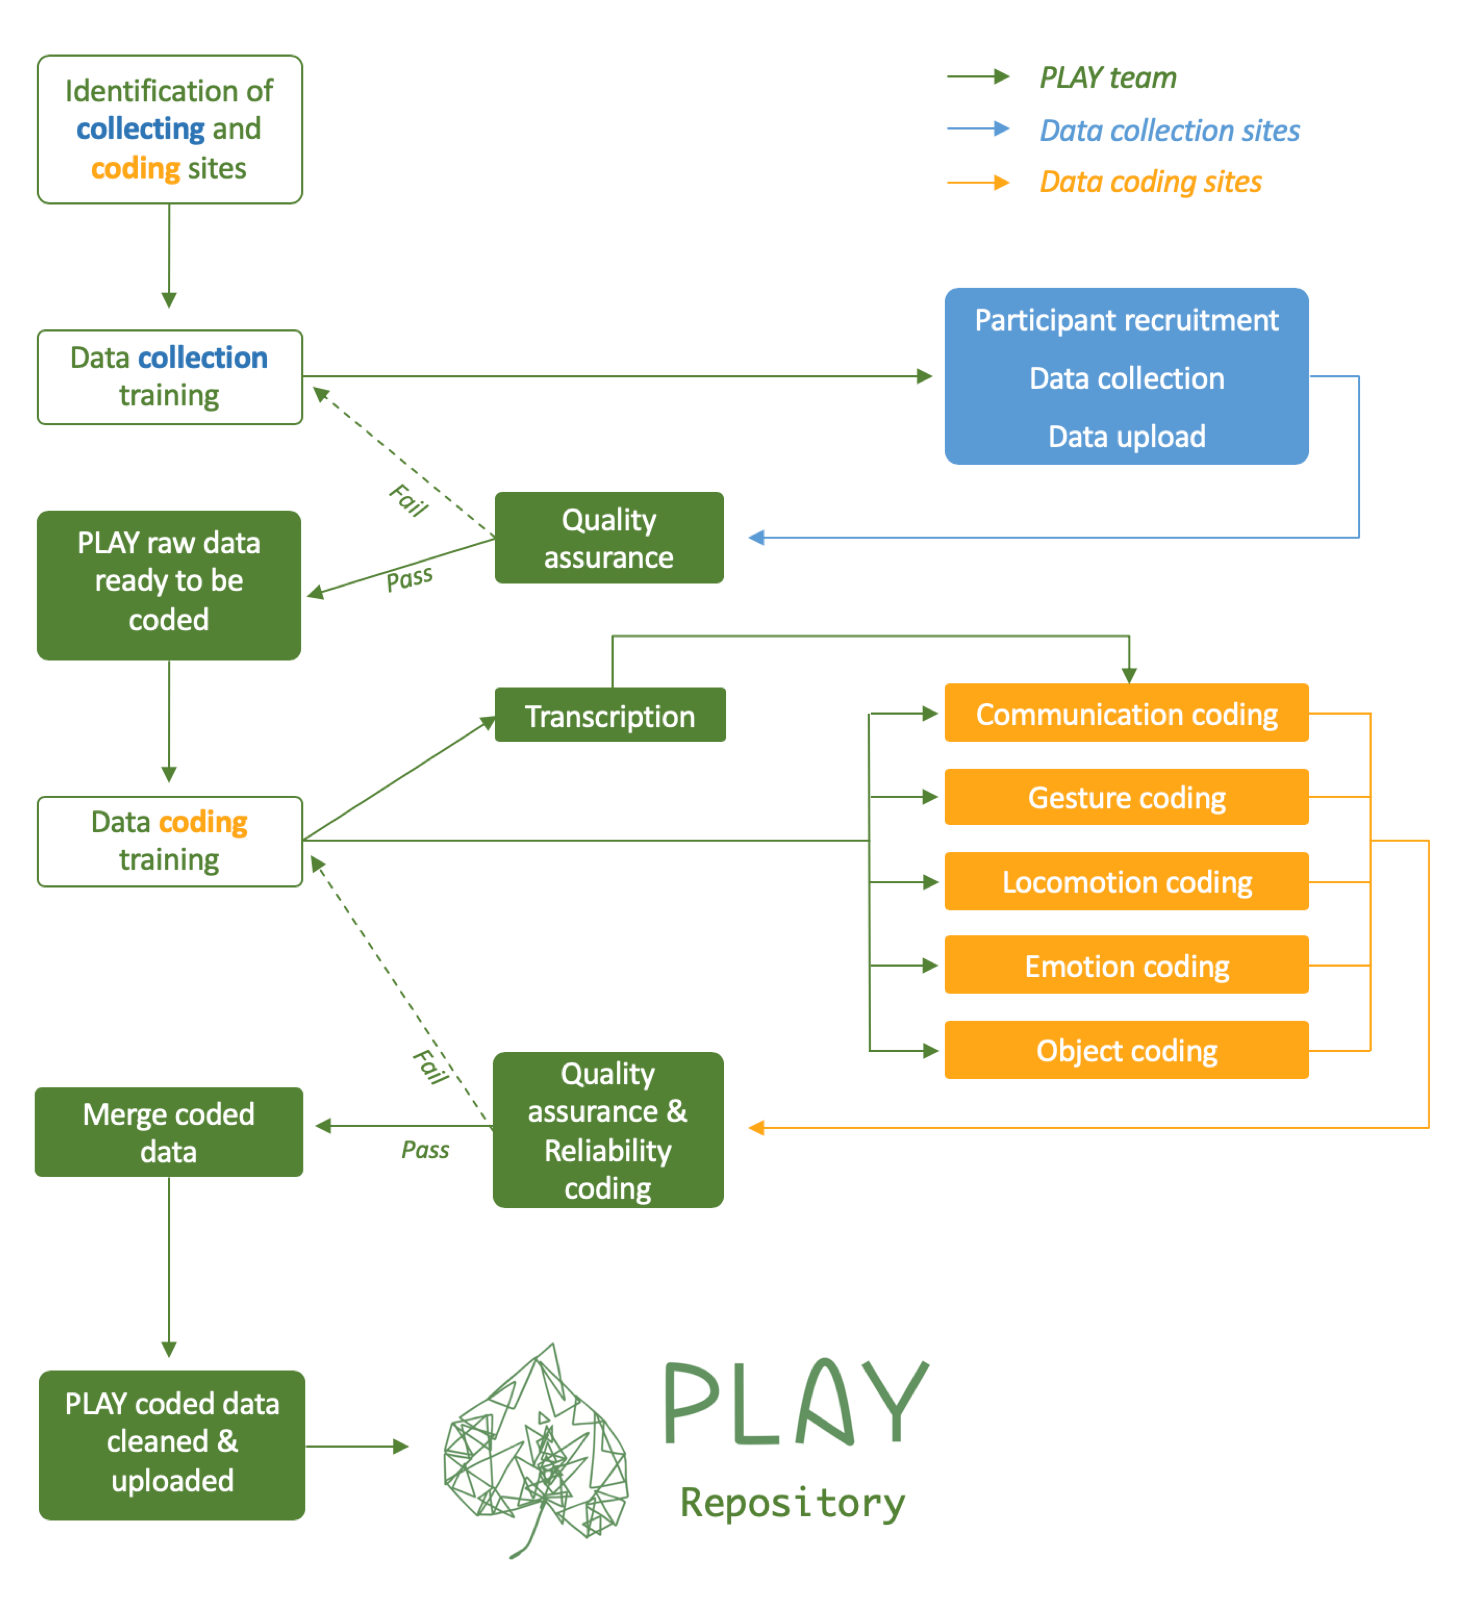
\includegraphics[width=0.7\linewidth]{img/overview-project}

\hypertarget{participants}{%
\section{Participants}\label{participants}}

The collaborating sites in PLAY perform a variety of roles (see \protect\hyperlink{people}{people} for details). Each site that performs a \textbf{collecting} role is pre-assigned to complete all of the collecting functions (see in blue below). This page contains detailed help for the recruitment of participants. Click here for information about the data collection and data upload processes.

PLAY aims to set new standards for conducting open, transparent, and reproducible behavioral science by i) publishing the protocol, and ii) making extensive use of video exemplars to demonstrate phenomena and illustrate behavioral codes. For confidentiality reasons, access to video exemplars is restricted to researchers with authorized access to \href{http://databrary.org}{Databrary}. To register for access, visit \url{http://databrary.org/register}.

Please ensure that you are \href{https://nyu.databrary.org/user/login}{\textbf{currently logged in at Databrary}} to view embedded video examples in this webpage and gain access to phone and home questionnaires.

\hypertarget{sampling}{%
\section{Sampling}\label{sampling}}

PLAY will produce a widely varied and rich set of data, most of which will be openly shared with the research community at the end of the five-year NIH grant period in late 2023. Infants' natural play in the home is characterized by tremendous variability including variations in: geographic location, climate, SES, maternal/paternal employment, childcare experiences, infants' and mothers' ages, language environment, physical layout and characteristics of the home, availability of media, toys for play, and so on. Researchers will be able to explore the effects of any/all such factors.

\hypertarget{inclusionexclusion-criteria}{%
\section{Inclusion/Exclusion Criteria}\label{inclusionexclusion-criteria}}

Although PLAY endeavours to sample as much of the rich variations that the collection sites present, based on conversations with the launch group and to ensure a sufficient sample size, we will limit variability along several dimensions. To be included in the PLAY sample of 900 sessions, participants must:

\begin{itemize}
\tightlist
\item
  be 12, 18, or 24 months of age (+/- 1 week)
\item
  be a single child (i.e., no living siblings)
\item
  come from English or Spanish monolingual or bilingual homes (i.e., no other language exposure in the home)
\item
  be born full-term (37-43 weeks), of normal birth weight (\textgreater= 5.5 lbs), without known disabilities
\item
  come from two-parent or single-parent households
\end{itemize}

Additionally, the mother must act as the caregiver during the one-hour natural interaction, which will be scheduled at a time when \emph{only} the mother and infant are present.

\hypertarget{collection-sites}{%
\section{Collection sites}\label{collection-sites}}

Data will come from 30 geographically diverse sites across the US representing rural, suburban, and urban communities with different races, ethnicities, and socio-economic status, including English- and Spanish-speaking households.

The aim is to collect data that approximate county-level demographic characteristics as reflected in U.S. Census data.

\hypertarget{map}{%
\subsection{Map}\label{map}}

\hypertarget{racial-composition}{%
\subsection{Racial composition}\label{racial-composition}}

\hypertarget{socio-economic-status}{%
\subsection{Socio-economic status}\label{socio-economic-status}}

\hypertarget{education}{%
\subsection{Education}\label{education}}

\hypertarget{languages-spoken}{%
\subsection{Languages spoken}\label{languages-spoken}}

\hypertarget{video-1}{%
\section{Video}\label{video-1}}

All data collections will be recorded on video.
Parents will be asked for their permission to share the video recordings and other data with the research community.
When that permission is granted the videos and related data will be shared with the research community via \href{http://databrary.org}{Databrary}:

\begin{itemize}
\tightlist
\item
  Adolph, K., Tamis-LeMonda, C., Gilmore, R.O. \& Soska, K. (2016). PLAY Project: NICHD Workshop (2016-12-16). Databrary. Retrieved August 23, 2018 from \url{http://doi.org/10.17910/B7.254}.
\item
  Adolph, K., Tamis-LeMonda, C. \& Gilmore, R.O. (2017). PLAY Project: Pilot Data Collections. Databrary. Retrieved August 23, 2018 from \url{https://nyu.databrary.org/volume/444}.
\item
  Adolph, K., Tamis-LeMonda, C., Gilmore, R.O. \& Soska, K. (2018). Play \& Learning Across a Year (PLAY) Project Summit (2018-06-29 Philadelphia). Databrary. Retrieved August 23, 2018 from \url{http://doi.org/10.17910/B7.724}
\end{itemize}

\hypertarget{full-play-home-visit-protocol---example}{%
\paragraph{Full PLAY home visit protocol - example}\label{full-play-home-visit-protocol---example}}

This is a video of the full PLAY home visit protocol that is available to authorized Databrary users, who may use clips or images from it in presentations for informational or educational purposes. You must be logged in to \href{http://databrary.org}{Databrary} to view it.

Full-length video of home visit

\leavevmode\vadjust pre{\hypertarget{fullvideohomevisit}{}}%
Your browser does not support html5 video.

\emph{NOTE: This participant was not the only child in the home, so would not meet inclusion criteria for PLAY.}

\hypertarget{parent-report-questionnaire-data}{%
\section{Parent-report (questionnaire) data}\label{parent-report-questionnaire-data}}

PLAY researchers will collect and share a substantial corpus of parent-report (questionnaire) data. The full set of self-report questions can be found \href{collection_homevisit_questionnaires.html}{here}.

\hypertarget{part-collection}{%
\part{Collection}\label{part-collection}}

\hypertarget{recruitment}{%
\chapter{Recruitment}\label{recruitment}}

\hypertarget{scheduling-visit}{%
\section{Scheduling visit}\label{scheduling-visit}}

To schedule a visit, you will be making two phone calls to each family: the initial recruiting call and the confirmation call (if the family agrees to participate). Depending on the availability of the mother, you will complete the \href{link\%20to\%20questionnaires}{participant paperwork}.

\hypertarget{initial-recruiting-phone-call}{%
\section{Initial recruiting phone call}\label{initial-recruiting-phone-call}}

\hypertarget{english_instructions}{%
\subsection*{English instructions}\label{english_instructions}}
\addcontentsline{toc}{subsection}{English instructions}

(See video at the end of the script)

Hi, may I speak with {[}MOM{]}?
My name is {[}CALLER NAME{]} and I'm calling from {[}LAB{]}. Like local businesses that are re-opening, university research activities are starting up again following local safety guidelines. I'm calling today about a home study on how moms and children interact with each other. We'd be visiting your home, and for your participation, you'd receive a \$50 gift card at the end of the session. Can I tell you more about the study and the safety precautions we have in place?

First, I have some questions to see if you and {[}CHILD{]} qualify for the study.

Does {[}CHILD{]} have any siblings?

\begin{itemize}
\tightlist
\item
  → \emph{If yes: \textbf{end call}.} In this study, we want to observe you and {[}CHILD{]} when it's only the two of you in the home. Is it possible to arrange a time when only you and {[}CHILD{]} are home for two hours?
\item
  → \emph{If no: continue}
\end{itemize}

What language(s) do you speak to {[}CHILD{]}?

\begin{itemize}
\tightlist
\item
  → \emph{If not ENGLISH or SPANISH: \textbf{end call}.} To control for differences in communication, we are looking for families who speak mainly English or Spanish. Would it be alright if we contacted you for other studies in the future?
\item
  → \emph{If mainly English/Spanish: continue}
\end{itemize}

Was {[}CHILD{]} born on his/her due date? (If not: How many weeks and days early/late was he/she?)

\begin{itemize}
\tightlist
\item
  → \emph{If more than 4 weeks early: \textbf{end call}.} In this study, we are currently looking for children born on term. Would it be alright if we contacted you for other studies in the future?
\item
  → \emph{If born on term (37-41 weeks): continue}
\end{itemize}

Has {[}CHILD{]} been diagnosed with any disability (cognitive, auditory, vision, motor)?

\begin{itemize}
\tightlist
\item
  → \emph{If yes: \textbf{end call}.} In this study, we are looking for typically developing children. Would it be alright if we contacted you for other studies in the future?
\item
  → \emph{If no: continue}
\end{itemize}

For this study, we are interested in learning about children's natural, everyday experiences in their homes. A researcher will visit you and {[}CHILD{]} in your home for about 2-3 hours. In the main part of the study, the researcher will video record you and {[}CHILD{]} for 1 hour as you go about your normal day. Then, we will ask you to take us through your home as we record the environment. Finally, we will ask you questions about your family and {[}CHILD{]}'s skills and routines. The data collected in this study are valuable and will be placed in a secure web-based library available only to researchers. The purpose is to share the data with experts in the field so that scientists can learn more about infant development.

To protect you and your family, the researcher is fully vaccinated and will wear a mask. We will not physically interact with you or your child, this study is just observational. Anything we bring into your home will be sanitized.

Does this sound like something you would be interested in participating in with {[}CHILD{]}?

\begin{itemize}
\tightlist
\item
  → \emph{If no to study or to sharing video on Databrary: \textbf{end call} } Okay, thank you. May we call you for other studies?
\item
  → \emph{If yes: continue}
\end{itemize}

The researcher in your home will wear a mask, but we'd ask that you and your child do not. It's important to see and record your facial expressions and a mask would block those. Would you be ok to not wear a mask?

\begin{itemize}
\tightlist
\item
  → \emph{If no: \textbf{end call} } Currently, we are only enrolling families who are okay with not wearing a mask. But is it okay, if we call you for other studies?
\item
  → \emph{If yes: continue}
\end{itemize}

Have you or anyone in your household had COVID or had physical interaction with someone who has tested positive for COVID in the last two weeks?

\begin{itemize}
\tightlist
\item
  → \emph{If yes: \textbf{end call} } Currently, we are only enrolling families who are symptom-free and had no interaction with anyone COVID positive. But is it okay, if we call you for this study again in a few months?
\item
  → \emph{If no: continue}
\end{itemize}

Great! Because we are interested in mother-infant routines, we'd like to find a time and date when we can observe just {\textbf{you and {[}CHILD{]}}} at home. It would be great if we can schedule a time that is not during a typical mealtime and when {[}CHILD{]} is usually awake. Is there a convenient time and day that works best for you that would be within these criteria?

\begin{itemize}
\tightlist
\item
  → \emph{If the date they are available puts child out of age range: \textbf{end call} } For this study, we are interested in studying specific age groups: 12-, 18-, and 24-month olds. Would it be possible for us to contact you in XX months to see if {[}CHILD{]} can participate then?
\item
  → \emph{If dates are available when child is still within eligible age range: continue}
\end{itemize}

So I have you and {[}CHILD{]} for our study on {[}DATE{]} at {[}TIME{]}.

Before the study, we have a few questions that we'd like to ask. It should only take about 5 minutes. We can either ask you now or when we call to confirm the study. What would you prefer?

\begin{itemize}
\tightlist
\item
  → \emph{If ready to answer now, continue (see video for Demographics Questionnaire below this list)}:

  \begin{itemize}
  \tightlist
  \item
    On your tablet, open Kobo toolbox and start a new questionnaire set
  \item
    Fill out participant information at top of new session
  \item
    ``Save as Draft'' after demographic questionnaire and home visit questionnaires
  \item
    Only hit ``Submit'' after filling out clean-up notes back in lab
  \item
    Here are links to view the demographic questionnaire  
  \item
    \emph{Please note that presentation and format will differ in the app.}
  \end{itemize}
\item
  → \emph{If not available now} When will be a good time to call back about the questions?

  \begin{itemize}
  \tightlist
  \item
    If another time work, schedule a 5-minute call to complete demographic questionnaire
  \item
    If difficult to find a time up to 2 days before visit, complete demographic questionnaire when confirming visit
  \end{itemize}
\end{itemize}

So I have you and {[}CHILD{]} for our study on {[}DATE{]} at {[}TIME{]}. We'll be calling you the day before (if study is on Monday: the Friday before) your appointment to confirm that that time still works for you. Have a great day!

Initial recruiting phone call

Your browser does not support html5 video.

 

Demographics questionnaire

Your browser does not support html5 video.

\hypertarget{spanish_instructions}{%
\subsection*{Spanish instructions}\label{spanish_instructions}}
\addcontentsline{toc}{subsection}{Spanish instructions}

(Ver video al final del guión)

Hola, ¿puedo hablar con {[}MAMÁ{]}?
Mi nombre es {[}NOMBRE DE PERSONA QUE LLAMA{]} y estoy llamando de {[}LAB{]}. Al igual que las empresas locales que están reabriendo, se están reiniciando las actividades de investigación de las universidades, siguiendo las pautas de seguridad locales. Estoy llamando hoy por un estudio de como madres e hijos interactúan en el hogar. Lo visitaríamos en su hogar y usted recibiría una tarjeta de regalo de \$50 al final de la sesión por su participación. ¿Puedo contarle más sobre el estudio y las precauciones de seguridad que tenemos?

Primero tengo unas preguntas para ver si usted y {[}NIÑO{]} califican para participar en este estudio.

¿{[}NIÑO{]} tiene hermanos?

\begin{itemize}
\tightlist
\item
  → En caso de si: finalice la llamada. Actualmente para este estudio estamos sólo incluyendo a hijos únicos. ¿Estaría bien si les contactamos para otros estudios más adelante?
\item
  → En caso de no: continúe
\end{itemize}

¿En que idioma(s) le habla usted a {[}NIÑO{]}?

\begin{itemize}
\tightlist
\item
  → Si no es INGLES o ESPAÑOL finalice la llamada. Para controlar diferencias de comunicación, estamos buscando familias que hablen primariamente inglés o español. ¿Estaría bien si les contactamos para otros estudios más adelante?
\item
  → Si hablan principalmente inglés/español : continúe
\end{itemize}

¿Nació {[}NIÑO{]} en su fecha de termino? (En caso de no: Cuántas semanas y/o días antes/después de su fecha de termino nació?)

\begin{itemize}
\tightlist
\item
  → Si nació más de 4 semanas antes: finalice la llamada. Actualmente para este estudio estamos buscando a niños que hayan nacido de termino. ¿Estaría bien si les contactamos para otros estudios más adelante?
\item
  → Si nació de termino (37-41 semanas): continúe
\end{itemize}

¿Ha sido {[}NIÑO{]} diagnosticado con alguna discapacidad (cognitiva, auditiva, visual, o motora)?

\begin{itemize}
\tightlist
\item
  → En caso de si: finalice la llamada. Actualmente para este estudio estamos buscando a niños con desarrollo típico. ¿Estaría bien si les contactamos para otros estudios más adelante?
\item
  → En caso de no: continúe
\end{itemize}

En este estudio estamos interesados en aprender sobre las experiencias rutinarias que los bebés tienen en sus hogares. Un investigador lo visitará a usted y a {[}NIÑO{]} en su hogar por aproximadamente 2-3 horas. En la parte principal del estudio, un investigador grabará en vídeo a usted y {[}NIÑO{]} por 1 hora mientras ustedes continúan con sus actividades rutinarias. A continuación, le pediremos recorrer su hogar mientras grabamos el espacio. Finalmente le haremos preguntas sobre su familia y las habilidades y rutinas de {[}NIÑO{]}. Los datos recolectados en este estudio son valiosos y serán colocados en una biblioteca privada en internet a la cual sólo tienen acceso los investigadores autorizados. El propósito es compartir los datos con expertos en el área para que los científicos puedan aprender más sobre el desarrollo infantil.

Para protegerlo a usted y a su familia, el investigador está completamente vacunado y usará una mascarilla. No interactuaremos físicamente con usted o con su hijo/a, este estudio es solo observacional. Todo lo que llevemos a su hogar será desinfectado.

¿Le interesaría participar en este estudio con {[}NIÑO{]}?

\begin{itemize}
\tightlist
\item
  → En caso de no querer participar en el estudio o estar dispuesto a compartir los videos en Databrary: finalice la llamada.\\
  Bueno, gracias. ¿Podemos contactarles para otros estudios?
\item
  → En caso de si: continúe.
\end{itemize}

El investigador usará una mascarilla mientras lo visite en su hogar, pero le solicitamos que usted y su hijo/a no usen. Es importante ver y registrar sus expresiones faciales y una mascarilla las bloquearía. ¿Estaría de acuerdo con no usar una mascarilla?

\begin{itemize}
\tightlist
\item
  → En caso de si: finalice la llamada. Actualmente, solo estamos reclutando familias que están de acuerdo con no usar una mascarilla. Pero, ¿está bien si lo llamamos para otros estudios?
\item
  → En caso de no: continúe
\end{itemize}

¿Usted o alguien en su hogar ha tenido COVID o ha interactuado físicamente con alguien que haya salido positivo por COVID en las últimas dos semanas?

\begin{itemize}
\tightlist
\item
  → En caso de si: finalice la llamada. Actualmente, solo estamos inscribiendo familias que no tienen síntomas y no han tenido interacción con nadie con COVID positivo. Pero, ¿está bien si lo volvemos a llamar para este estudio en unos meses más?
\item
  → En caso de no: continúe
\end{itemize}

¡Genial! Debido a que estamos interesados en las rutinas de madres e hijos, nos gustaría encontrar un día y hora en el cual podamos observar sólo a usted y {[}NIÑO{]} en su hogar. Seria bueno si pudiéramos programar la visita a una hora que no sea durante el horario de comidas y cuando {[}NIÑO{]} esta generalmente despierto. ¿Hay algún día y hora que sea conveniente para usted donde se cumplan estos criterios?

\begin{itemize}
\tightlist
\item
  → Si en la fecha en la cual están disponibles el bebé ya esta fuera de el rango de edad: Para este estudio estamos interesados en estudiar grupos de edad específicas: 12-, 18, y 24- meses. ¿Estaría bien si les contactamos en XX meses para ver si {[}NIÑO{]} puede participar entonces?
\item
  → Si el niño esta en el rango de edad para la fecha en la cual están disponibles: continúe
\end{itemize}

Por ultimo, tenemos un cuestionario que solo tomará 5 minutos necesitamos completar antes de nuestra visita. Podemos preguntarle las preguntas ahora o cuando llamemos para confirmar el estudio. ¿Qué prefiere usted?

\begin{itemize}
\tightlist
\item
  → En caso de que madre pueda responder las preguntas ahora, continúe (see video for Demographics Questionnaire below this list):

  \begin{itemize}
  \tightlist
  \item
    Abra un nuevo cuestionario en Kobo toolbox en el Tablet.
  \item
    Rellene la información del participante en una nueva sesión.
  \item
    Luego de completar el cuestionario demográfico guarde como ``sabe as draft''.
  \item
    Solo oprima ``submit'' al completar todas las notas luego de la visita.
  \item
    Lista de preguntas del cuestionario demográfico  
  \item
    Por favor tenga presente que el formato será distinto que en la aplicación.
  \end{itemize}
\item
  → En caso de que madre no pueda responder las preguntas en este momento, Cuando seria un buen momento para llamarla nuevamente cuando usted tenga tiempo para responder estas preguntas?

  \begin{itemize}
  \tightlist
  \item
    Si puede en otro momento, programe una llamada de 5-minutos para completar el cuestionario demográfico.
  \item
    Si es difícil coordinar una llamada, complete el cuestionario al llamar para confirmar la visita.
  \end{itemize}
\end{itemize}

Entonces tenemos agendada la visita para el día {[}FECHA{]} a las {[}HORA{]}. La llamaremos el día anterior /el viernes anterior (si la visita es un lunes) para confirmar que aun están disponibles para a la visita. Excelente, que tenga un buen día!

Initial recruiting phone call

Your browser does not support html5 video.

 

Demographics questionnaire

Your browser does not support html5 video.

\hypertarget{initial-recruiting-voicemail}{%
\subsection*{Initial recruiting voicemail}\label{initial-recruiting-voicemail}}
\addcontentsline{toc}{subsection}{Initial recruiting voicemail}

If you reach the family's voicemail, please leave the following message:

\hypertarget{english-script}{%
\subsubsection*{English script}\label{english-script}}
\addcontentsline{toc}{subsubsection}{English script}

Hi, this message is for {[}MOM{]}. My name is {[}NAME{]} and I'm calling from {[}LAB{]}. I'm calling because we have a fun study for {[}12 / 18 / 24{]}-month-olds and {[}CHILD{]} is the perfect age. You would receive a \$50 gift card for participating in the study and if you are interested in hearing more, please give us a call back. Our phone number is {[}XXX-XXX-XXXX{]}. Thank you and we hope to hear from you soon!

Initial recruiting voicemail

Your browser does not support html5 video.

\hypertarget{spanish-script}{%
\subsubsection*{Spanish script}\label{spanish-script}}
\addcontentsline{toc}{subsubsection}{Spanish script}

Hola, este mensaje es para {[}MAMÁ{]}. Mi nombre es {[}NOMBRE{]} y estoy llamando de {[}LAB{]}. Estoy llamando porque tenemos un estudio para niños de {[}12 / 18 / 24{]}- meses y {[}NIÑO{]} tiene la edad perfecta. Usted recibiría una tarjeta de regalo de \$50 por participar en este estudio y si usted esta interesado en saber más sobre este estudio, por favor llámenos de vuelta. Nuestro número de teléfono es {[}XXX-XXX-XXXX{]}. ¡Gracias y esperamos su llamada!

Initial recruiting voicemail

Your browser does not support html5 video.

\hypertarget{initial-recruiting-email}{%
\section{Initial recruiting email}\label{initial-recruiting-email}}

If you will be contacting the family over email, you may use the following template:

\hypertarget{english-template}{%
\subsection*{English template}\label{english-template}}
\addcontentsline{toc}{subsection}{English template}

\begin{verbatim}
Dear [MOM],
  
I am writing from the [LAB] to tell you about a fun study that [CHILD] would be perfect for!

For this study, we are interested in learning about babies' natural, everyday experiences in their homes — such as the toys they play with and the places they go. A researcher will visit you and [CHILD] in your home, and the two of you will be video recorded as you go about your day. The visit lasts about 2-3 hours, and you will receive a $50 gift card at the end of the session.
To protect you and your family, the researcher is fully vaccinated and will wear a mask. We will not physically interact with you or your child, this study is just observational. Anything we bring into your home will be sanitized.
If you are interested in participating, would like more information, or have any questions, feel free to contact us by email or phone. Our phone number is [XXX-XXX-XXXX]. We look forward to hearing from you soon!

Thank you, 
[LAB]
\end{verbatim}

\hypertarget{spanish-template}{%
\subsection*{Spanish template}\label{spanish-template}}
\addcontentsline{toc}{subsection}{Spanish template}

\begin{verbatim}
Estimada [MAMÁ],

Le estamos escribiendo desde [LAB] para contarle sobre un estudio de investigación que sería ideal para [NIÑO].

Para este estudio, estamos interesados en conocer las experiencias cotidianas y naturales de los niños en sus hogares – los juguetes con los que juegan y los lugares a los que van en su hogar. Un investigador lo visitará a usted y a [NIÑO] en su hogar, y ustedes serán filmados mientras realizan sus actividades diarias. Cada visita dura aproximadamente 2-3 horas, y usted recibirá una tarjeta de regalo de $50 por su participación.
Para protegerlo a usted y a su familia, el investigador está completamente vacunado y usará una mascarilla. No interactuaremos físicamente con usted o con su hijo/a, este estudio es solo observacional. Todo lo que llevemos a su hogar será desinfectado.
Si usted está interesada en participar, desea más información o tiene alguna pregunta, no dude en contactarnos por correo electrónico o por teléfono. Nuestro número [XXX-XXX-XXXX]. ¡Esperamos tener noticias de usted pronto!

Gracias,
[LAB]
\end{verbatim}

\hypertarget{home-visit}{%
\chapter{Home Visit}\label{home-visit}}

Now that you have set your target participant sample and completed all the steps listed in the \href{collection_recruitment.html}{recruitment} process, these instructions will help you prepare for your participant home visit.

Please ensure that you are \href{https://nyu.databrary.org/user/login}{\textbf{currently logged in at Databrary}} to view protected content in this webpage. For confidentiality reasons, access to video exemplars is restricted to researchers with authorized access to \href{http://databrary.org}{Databrary}. To register for access, visit \url{http://databrary.org/register}.

At the end of every home visit (for each participant), you will upload the following:

\begin{enumerate}
\def\labelenumi{\arabic{enumi}.}
\tightlist
\item
  \textbf{exactly 4 videos} (to your Databrary repository)
  ~ - One-hour naturalistic play (include: decibel measure, shoes if child is wearing them in the house)
  ~ - House walk-through (include: measurements of each room, sleeping arrangements, clothing, books, toys, shoes if child is barefoot)
  ~ - 5-min structured play (focus on child and mom, even if they leave mat area)
  ~ - Questionnaires (set up camera on tripod, focus on mom)
\item
  \textbf{exactly 1 decibel meter file} (to your Databrary repository)
\item
  \textbf{exactly 3 questionnaire files} (through the KoBo Toolbox app)
  ~ - demographics questionnaire
  ~ - home visit questionnaire
  ~ - post-visit notes
\end{enumerate}

\hypertarget{arrival-introduction}{%
\section{Arrival introduction}\label{arrival-introduction}}

\emph{\textbf{Note}: Experimenters should always act in a professional and respectful manner when interacting with the participants and while in the home. Do not make comments or react to anything in front of the mom to make her feel uncomfortable. All families should feel that their participation in the study is meaningful.}

Say: Hi, my name is {[}NAME{]} and I'm visiting from {[}INSTITUTION{]}. Thanks for letting us come to your home today!
    Hola, mi nombre es {[}NAME{]} y vengo de {[}INSTITUTION{]}. ¡Gracias por recibirnos hoy en su hogar!

\begin{itemize}
\tightlist
\item
  Ask if you should take your shoes off.
\item
  Ask for good place (i.e.~out of child's reach) to put backpack and coat.
\item
  Do not leave the tripod and other equipment lying around.
\item
  Do not engage or warm up to the baby. Just need to make mom feel comfortable.
\end{itemize}

\hypertarget{consent-to-participate}{%
\section{Consent to participate}\label{consent-to-participate}}

Experimenter should explain the study and ask mom to sign the consent.

Say: The visit has a few parts. I'll begin by video-recording you and {[}CHILD{]} as you go about your day. I will video-record you both for one hour. Afterwards, I'll ask you to give me a walk-through of your home that I will record on video to get a sense of the places {[}CHILD{]} goes and things that he/she plays with. I'll also be measuring the dimensions of each room. Then, I will ask you and {[}CHILD{]} to play with some toys that I brought with me. Finally, I will ask you some general questions about your family and home, and about {[}CHILD{]}'s skills and routines. Everything will be video-recorded and the visit will last for no more than three hours. You will receive \$50 for your participation at the end. Do you have any questions? Okay, great. Here is the consent form that explains everything I just said. Please read it through and then print and sign your name on the back.
    Esta visita tiene varias partes. Comenzaré grabándolos a usted y {[}CHILD{]} por una hora, mientras realizan sus actividades cotidianas. Después, le pediré que me dé un recorrido por su hogar mientras grabo los espacios, para tener una idea de los lugares donde él/ella va y las cosas con las que juega. También mediré las dimensiones de cada cuarto. Luego, les pediré a usted y a {[}CHILD{]} que jueguen con unos juguetes que traje conmigo. Finalmente, le haré algunas preguntas generales acerca de su familia y su hogar, y sobre las habilidades y rutinas de {[}CHILD{]}. Todo será grabado en video y la visita no durará más de 3 horas. Por participar usted recibirá \$50 al final de la visita. ¿Tiene alguna pregunta? ¡Muy bien! Aquí tiene el formulario de consentimiento que explica todo lo que le he dicho. Por favor léalo y luego en el reverso escriba su nombre y firme.

Obtain consent - Spanish

Your browser does not support html5 video.

\hypertarget{one-hour-natural-play-video-noise-measurement}{%
\section{One-hour natural play video \& noise measurement}\label{one-hour-natural-play-video-noise-measurement}}

\hypertarget{decibel-meter}{%
\subsection{Decibel Meter}\label{decibel-meter}}

Say: We would like to measure the environmental noise levels. Is there a good place where I can put this measuring device where your child cannot reach? The tablet only measures the environmental noise levels and not what you're actually saying.
    Queremos medir los niveles de ruido ambiental. ¿Hay algún lugar donde pueda colocar este dispositivo donde su hijo/a no lo pueda alcanzar? La tableta solo mide el ruido ambiental y no lo que usted está diciendo.

\begin{itemize}
\tightlist
\item
  Set up tablet, put in microphone.
\item
  Ensure that ``Audio Tool'' is force closed.
\item
  Place device in the most central place in the home (e.g., living room).
\item
  The microphone should be facing towards the room (e.g., away from walls) and propped up on the tablet case so that it is \textbf{not} lying flat against the surface of the space.
\end{itemize}

\hypertarget{one-hour-natural-play-video}{%
\subsection{One-Hour Natural Play Video}\label{one-hour-natural-play-video}}

General Recording Guidelines

\begin{itemize}
\tightlist
\item
  Aim to get 60 minutes of uninterrupted natural play recoding, in addition to the time you take to give instructions, record the decibel meter and shoes.
\item
  Keep camera on the child at all times. Specifically, ensure that the child's whole body is visible on camera. If mom is in frame, capture as much of her body as possible without compromising the view of the child.
\item
  Record in front or to the side of the child as much as possible.
\item
  Do not zoom in.
\item
  Always try to stay toward the edge of rooms and doorways. You do not want to influence child to interact with you, or get in child's way.
\item
  Remain at as far a distance as possible (\textasciitilde3 to 5 m, hugging the wall) so that the child is not distracted by your presence.
\item
  Try not to interact with the child or make eye contact with the child. Just watch through the viewfinder of the camera.
\item
  If mom asks to pause the camera, ask for permission to point the camera away so you can continue recording audio.
\end{itemize}

Say: So I'm going to start recording now.
    Voy a empezar a grabar ahora.

One hour natural play - view of child

Your browser does not support html5 video.

 

One hour natural play - view of experimenter

Your browser does not support html5 video.

Begin recording and say: For the next hour, do anything you would typically do as if I weren't here. Try to ignore me as much as possible and I will stay out of the way. I will also try not to respond to you and {[}CHILD{]} so that he/she is not distracted. You can go anywhere in your home but we just ask you to remain indoors. You can play together or not, you can do chores, watch TV, talk on the phone, give him/her a bath or snack. The idea is to capture what your typical day is like. And as a reminder, I'm just here to record so you will be in charge of {[}CHILD{]}'s safety.
    En la próxima hora, haga cualquier cosa que usted haría típicamente si yo no estuviera aquí. Intente ignorarme lo más posible y yo me mantendré fuera de su camino. También intentaré no responderle a usted o a {[}CHILD{]} para no distraerlo/la. Puede ir a cualquier lugar en su hogar, solo pedimos que se mantenga adentro. Pueden jugar juntos o no, puede hacer los quehaceres, ver televisión, hablar por teléfono, darle un baño o una merienda a {[}CHILD{]}. La idea es capturar su día típico. Le recuerdo que solo estoy aquí para grabar y usted está a cargo de la seguridad de {[}CHILD{]}.

One hour natural play - view of child - Spanish

Your browser does not support html5 video.

 

Point camera at the tablet while opening ``Audio Tool'' (the application immediately starts recording noise levels upon startup).

Turn ON decibel meter

Your browser does not support html5 video.

After opening the app, quickly point the camera at the child and start timing for the one-hour natural play video. Note the time on the viewfinder of the camera and record for an additional 60 minutes.

\emph{Note: The instructions and tablet set up should take no longer than 5-minutes.}

At the end of the one-hour recording, say: Great, we are done with the one-hour recording! ¡Excelente, hemos terminado la grabación de una hora!

With camera in hand (and still recording), walk over to where the tablet was placed, and hit the ``save'' button on ``Audio Tool''.

Turn OFF decibel meter

Your browser does not support html5 video.

\hypertarget{shoes}{%
\paragraph{Shoes}\label{shoes}}

\begin{itemize}
\tightlist
\item
  If child was wearing shoes during the recording, say Could I get a close-up of the shoes {[}CHILD{]} has been wearing? ¿Puedo grabar más de cerca los zapatos que {[}CHILD{]} tiene puestos? . Ask mom to remove the shoes, video-record the shoes after the session; take them off child and video the bottom, side, and top views. Focus the camera on the shoes and comment on shoe type, sole (hard, soft), heel (if any), and other observations.
\item
  If the child was \emph{not} wearing shoes during the one-hour natural play video, record the shoes during the house walk-through.
\end{itemize}

Shoes

Your browser does not support html5 video.

Then stop video recording on the camera. Now that the camera is off, name the audio file with the site name and subject number (e.g.~NYU\_001) and close the ``Audio Tool'' app.

\hypertarget{video-house-walk-through-while-measuring-rooms}{%
\section{Video House Walk-through while measuring rooms}\label{video-house-walk-through-while-measuring-rooms}}

Start recording and say: Now, we would like to see the space that {[}CHILD{]} gets to explore throughout the day. Please walk me through your home as I follow with a camera, and take measurements of the spaces. As we walk around, please show me where you keep any objects --- toys, books, sippy cups, anything like that --- that {[}CHILD{]} might interact with regularly. Please show me where you keep his/her clothes and shoes to give us an idea of the kinds of things he/she wears.
    Ahora nos gustaría ver el espacio que {[}CHILD{]} tiene para explorar durante el día. Por favor guíeme por su hogar mientras la sigo con una cámara y tomo medidas de los espacios. Mientras recorremos su hogar, por favor muéstreme donde guarda cualquier objeto- juguetes, libros, vasitos, cualquiera de las cosas con que {[}CHILD{]} interactúa regularmente. Por favor muéstreme donde guarda la ropa y los zapatos de él/ella para tener una idea de las cosas que él/ella viste.

House walkthrough - English

Your browser does not support html5 video.

House walkthrough - Spanish

Your browser does not support html5 video.

Ensure that all of experimenter's personal items, recording equipment, yoga mat and toys for structured play are stored out of sight.

Video capture tips:

\begin{itemize}
\tightlist
\item
  Watch recording through viewfinder to ensure that the view is not blurry or shaky\\
\item
  Move the camera slowly and walk slowly\\
\item
  A clear and steady view, free of blurriness and shakiness, is necessary for detailed coding of the home environment
\item
  The laser measure device does not work against reflective surfaces (mirrors, glass walls, etc), so point to a non-reflective surface or measure from the reflective surface towards the opposite direction.
\end{itemize}

About room measurements:

\begin{itemize}
\tightlist
\item
  You will measure all rooms in the house while you do the video walkthrough\\
\item
  A room is any space used by someone on a regular basis - bedrooms, kitchens, bathrooms, basements - they don't need to have windows\\
\item
  A room has to have a clear demarcation (e.g., a wall or an entry). A space is considered to be a room if it has a minimum of 3 walls.
\item
  If the room has a short divider (e.g., when a kitchen and a living room are divided by a counter), count as one big room and measure accordingly.
\end{itemize}

Steps:

\begin{enumerate}
\def\labelenumi{\arabic{enumi}.}
\tightlist
\item
  Start at the entrance of the home.
\item
  Pause at the entrance of each room.
\item
  Audibly name the room by its function (e.g., This is where {[}CHILD{]} sleeps).
\item
  First, get as much of the \textbf{Entire Room} in frame as possible. Keep the camera zoomed out and make sure to capture the ceiling and the floor of the room.
\item
  Next, pan the camera SLOWLY from \textbf{Left to Right}.
\item
  Then, pan the camera to \textbf{Floor}, name the different types of surfaces in the space (hardwood, plush carpet, thin rug, linoleum, tile, etc.), and then pan to the \textbf{Ceiling}.
\item
  Ask parent if child spends time in each room: Does {[}CHILD{]} spend any time in this room? ¿{[}CHILD{]} pasa algo de tiempo en este cuarto?
\item
  Ask parent about child's objects in the room: Do you keep anything for {[}CHILD{]} in this room? (If yes) Would you mind showing me? ¿Guarda algo para {[}CHILD{]} en este cuarto? (If yes) ¿Me lo puede mostarar por favor?
\item
  \textbf{Ensure during the house walkthrough that the parent provides information on all of the following:}

  \begin{itemize}
  \tightlist
  \item
    \emph{Children's Sleeping Arrangements.} Please show me where {[}CHILD{]} typically sleeps. Por favor muéstreme donde {[}CHILD{]} duerme típicamente.
  \item
    \emph{Child's Clothes.} Please show me where you keep {[}CHILD{]}'s clothes. Por favor muéstreme donde guarda la ropa de {[}CHILD{]}.
  \item
    \emph{Child's Shoes.} Please show me where you keep {[}CHILD{]}'s shoes. Por favor muéstreme donde guarda los zapatos de {[}CHILD{]}.
  \item
    \emph{Child's Books.} Please show me where you keep {[}CHILD{]}'s books. Por favor muéstreme donde guarda los libros de {[}CHILD{]}.
  \item
    \emph{Child's Toys.} Please show me where you keep {[}CHILD{]}'s toys. Por favor muéstreme donde guarda los juguetes de {[}CHILD{]}.
  \end{itemize}
\item
  Film the \textbf{Location} of the storage space (drawer, toy chest, cabinet) in clear context of the rest of the room. Then, SLOWLY and CLEARLY film the \textbf{Contents} of the storage space to show what is inside of it, zooming in if needed. (Overhead view for bed, crib, drawers, toy chest, etc.; Zoomed in side view for cabinet, closet, bookshelf, etc.)
\item
  Hold the camera in one hand while you take measurements of the room using the other.

  \begin{itemize}
  \tightlist
  \item
    Turn measure on by pressing ON/DIST button. Make sure the laser beam is visible.
  \item
    Measure wall to wall, lengthwise and widthwise.
  \item
    If a room has an odd or asymmetrical shape (i.e., any shape other than a rectangle or a square), measure the largest rectangle or square area of the room.
  \item
    Place the base of the laser flat on the wall, push ON/DIST againt to send the beam across the room (avoid moldings, door castings, reflective surfaces)
  \item
    Repeat the above for the second dimension (length or width)
  \item
    Focus camera on laser measure for each measure and read numbers out loud with units (e.g.~eight point five feet)
  \end{itemize}
\item
  Do ** \emph{NOT} ** turn off the camera when walking to next room.
\item
  Walk SLOWLY.
\item
  When all rooms are recorded, walk back to the entrance of the home and then stop recording.
\end{enumerate}

\protect\hyperlink{faqs_walkthrough}{FAQs about House Walk-through}

\hypertarget{five-minute-structured-mother-child-play}{%
\section{Five-minute Structured Mother-Child Play}\label{five-minute-structured-mother-child-play}}

Structured Play - English

Your browser does not support html5 video.

 

Structured Play - Spanish

Your browser does not support html5 video.

Say: Now I would like you to play with your child for about 5 minutes with these toys. We always clean these toys before and after each visit. I have a mat that I'm going to ask you to sit on. Where's a good place for me to put it?
    Ahora le pediré que por favor juegue con su hijo/a durante unos 5 minutos con estos juguetes. Siempre limpiamos los juguetes antes y después de cada visita. Tengo una estera/alfombra en la cual le voy a pedir que se siente. ¿Dónde es un buen lugar para ponerla?

Place the mat on a clearing on the floor.

Start recording and say: Please sit next to {[}CHILD{]} on this mat. I'll give you a set of toys. Please play with {[}CHILD{]} however you like for 5 minutes.
    Por favor siéntese al lado de {[}CHILD{]} en esta estera/alfombra. Le daré unos juguetes. Por favor juegue con {[}CHILD{]} por 5 minutos como usted quiera.

\begin{itemize}
\tightlist
\item
  If the child is playing with a different toy before the recording, ask mom if she can put the toy away.
\item
  Hand tote bag with toys to mom. Quickly point the camera at the child and mom and note the time on the viewfinder. Record for an additional 5 minutes.
\item
  Record so that the child and mother's entire bodies - faces, eyes, and hands - are captured. If child stands up, make sure to capture the feet. If you are in a position from which you cannot capture the full face and both eyes, position yourself to capture a profile view.
\item
  If child and mom are separated at any point, focus camera on child.
\item
  Use timer on camera to time engagement.
\item
  After 5 minutes, say ``Great job! We can now move on to the questionnaires.''
\item
  If the child is still playing with the toys after 5 minutes, let the child play and continue on to the questionnaires.
\end{itemize}

\protect\hyperlink{faqs_structured_play}{FAQs about House Structured Play}

\hypertarget{questionnaires}{%
\section{Questionnaires}\label{questionnaires}}

\protect\hyperlink{faqs_questionnaires}{FAQs about Questionnaires}

\hypertarget{visit-wrap-up}{%
\section{Visit wrap-up}\label{visit-wrap-up}}

\begin{itemize}
\tightlist
\item
  Give mom the payment
\item
  Ensure that mom has copies of the consent and Databrary forms
\item
  Collect and pack all equipment and paperwork from the house
\item
  Thank mom for letting us come to her home!
\end{itemize}

\hypertarget{full-play-home-visit-protocol---example-1}{%
\section{Full PLAY home visit protocol - example}\label{full-play-home-visit-protocol---example-1}}

Here is a video of the full PLAY home visit protocol.

Full-length video of home visit

\leavevmode\vadjust pre{\hypertarget{fullvideohomevisit}{}}%
Your browser does not support html5 video.

\emph{NOTE: This participant was not the only child in the home, so would not meet inclusion criteria for PLAY.}

\hypertarget{post-visit}{%
\chapter{Post-visit}\label{post-visit}}

\hypertarget{post-visit-notes-clean-up-and-upload}{%
\section{Post Visit notes, Clean up, and Upload}\label{post-visit-notes-clean-up-and-upload}}

After each visit, when you arrive back at your lab, complete all the following steps on the day you collected the data or on the very next day.

\begin{enumerate}
\def\labelenumi{\arabic{enumi}.}
\tightlist
\item
  Submit home questionnaires.

  \begin{itemize}
  \tightlist
  \item
    Open the completed questionnaire on the tablet and hit the submit button. Tablet must be connected to wifi.\\
  \end{itemize}
\item
  Complete and submit PLAY Post-Visit Notes

  \begin{itemize}
  \tightlist
  \item
    \url{https://ee.kobotoolbox.org/x/\#2cAYQt3z}\strut \\
  \end{itemize}
\item
  Upload all videos from the visit to Databrary onto your university's PLAY volume.
  Use the naming convention for each of the four videos. Use your 5 letter code for SITE. Use 3 digits for subject number (\#\#\#).

  \begin{itemize}
  \tightlist
  \item
    Name the session as: PLAY\_SITE\_\#\#\#\\
  \item
    Name the Natural Play video as: PLAY\_SITE\_\#\#\#\_NaturalPlay\\
  \item
    Name the House Walkthrough video as: PLAY\_SITE\_\#\#\#\_HouseWalkthrough\\
  \item
    Name the Structured Play video as: PLAY\_SITE\_\#\#\#\_StructuredPlay\\
  \item
    Name the Questionnaires video as: PLAY\_SITE\_\#\#\#\_Questionnaires\\
  \end{itemize}
\item
  Select appropriate release level for session in Databrary.

  \begin{itemize}
  \tightlist
  \item
    \url{https://www.databrary.org/resources/guide/investigators/release/release-levels.html}
  \end{itemize}
\item
  Make sure that all fields on Databrary are filled out.
  If visit is excluded mark as:

  \begin{itemize}
  \tightlist
  \item
    Pilot
  \item
    Atypical
  \item
    Out of age range
  \item
    Cancelled (if visit was cancelled)
  \item
    Experimental error (equipment malfunction)
  \item
    Incomplete
  \end{itemize}
\item
  Submit decibel data.

  \begin{itemize}
  \tightlist
  \item
    Please access the decibel app file on your tablet (located in the ``AudioTool'' folder in the File Manager). Select the decibel file from this home visit session.
  \item
    Select ``Share with Save to Drive'', navigate to the audio file folder for your site (e.g., `audio\_NYUNI') and drop your file in that location.
  \item
    Name the file as follows: PLAY\_SITE\_\#\#\#
  \item
  \end{itemize}
\item
  Fill out form to submit session for quality assurance. \url{https://forms.gle/dyqtsAxx3D8LJuTr8}.
\item
  Clean equipment.

  \begin{itemize}
  \tightlist
  \item
    Wash all toys and equipment thoroughly.
  \item
    Wipe down yoga mat.
  \item
    Once videos have been uploaded, delete all videos from SD card.
  \item
    Make sure to put away all equipment to have ready for a next visit.
  \end{itemize}
\end{enumerate}

\begin{center}\rule{0.5\linewidth}{0.5pt}\end{center}

At the end of every home visit (for each participant), you will upload the following:

\begin{enumerate}
\def\labelenumi{\arabic{enumi}.}
\tightlist
\item
  \textbf{exactly 4 videos} (to your Databrary repository)
  ~ - One-hour naturalistic play (include: decibel measure, shoes if child is wearing them in the house)
  ~ - House walk-through (include: measurements of each room, sleeping arrangements, clothing, books, toys, shoes if child is barefoot)
  ~ - 5-min structured play (focus on child and mom, even if they leave mat area)
  ~ - Questionnaires (set up camera on tripod, focus on mom)
\item
  \textbf{exactly 1 decibel meter file} (to your Databrary repository)
\item
  \textbf{exactly 3 questionnaire files} (through the KoBo Toolbox app)
  ~ - demographics questionnaire
  ~ - home visit questionnaire
  ~ - post-visit notes
\end{enumerate}

\hypertarget{frequently-asked-questions}{%
\chapter{Frequently Asked Questions}\label{frequently-asked-questions}}

\textbf{Pro tip:} The easiest way to find answers to your question is to ``Find'' (\texttt{Cmd+F} on a Mac or \texttt{Ctrl+F} on Windows) and type the simplest form of the word you're looking for. For example, searching for the word \texttt{dog} will bring up the FAQ ``What if doorbell rings for the dog walker, delivery, etc.?''

\hypertarget{faq-about-scheduling-and-recruitment}{%
\section{FAQ about scheduling and recruitment}\label{faq-about-scheduling-and-recruitment}}

\hypertarget{how-far-can-we-go-to-visit-a-family-for-a-home-visit}{%
\paragraph*{How far can we go to visit a family for a home visit?}\label{how-far-can-we-go-to-visit-a-family-for-a-home-visit}}
\addcontentsline{toc}{paragraph}{How far can we go to visit a family for a home visit?}

\begin{itemize}
\tightlist
\item
  The only restriction is that the family must live in the same state as the site. It is up to the PI and research team what the maximum distance they want to travel is. Depending on the location, some sites may have longer commute times than others.
\end{itemize}

\hypertarget{are-travel-expenses-i.e.-public-transportation-or-gas-reimbursed}{%
\paragraph*{Are travel expenses (i.e.~public transportation or gas) reimbursed?}\label{are-travel-expenses-i.e.-public-transportation-or-gas-reimbursed}}
\addcontentsline{toc}{paragraph}{Are travel expenses (i.e.~public transportation or gas) reimbursed?}

\begin{itemize}
\tightlist
\item
  Please speak with your site PI about what travel expenses can be covered and how to obtain reimbursements.
\end{itemize}

\hypertarget{if-mom-asks-if-she-needs-to-be-alone-during-the-study-and-if-fatherauntnannyetc.-can-be-anywhere-at-home-during-the-study}{%
\paragraph*{If mom asks if she needs to be alone during the study, and if father/aunt/nanny/etc. can be anywhere at home during the study}\label{if-mom-asks-if-she-needs-to-be-alone-during-the-study-and-if-fatherauntnannyetc.-can-be-anywhere-at-home-during-the-study}}
\addcontentsline{toc}{paragraph}{If mom asks if she needs to be alone during the study, and if father/aunt/nanny/etc. can be anywhere at home during the study}

For the first 90 minutes of this study, we are interested in how mothers and children interact. It should only be you and your child during the first half of our visit. If father/aunt/nanny/etc isn't able to stay out of the home for the full time that we're there, they can come back for the last hour.

\hypertarget{if-mom-specifically-says-that-the-fatheranyone-works-at-home-and-that-its-inconvenient-for-them-to-leave}{%
\paragraph*{If mom specifically says that the father/anyone works at home and that it's inconvenient for them to leave}\label{if-mom-specifically-says-that-the-fatheranyone-works-at-home-and-that-its-inconvenient-for-them-to-leave}}
\addcontentsline{toc}{paragraph}{If mom specifically says that the father/anyone works at home and that it's inconvenient for them to leave}

We really want just mom and child in the house during the first half of the visit. If there is a separate room with a door that the child never goes into (and that the father/person wouldn't leave anytime during the first half of the visit), then it's ok. But, if it's only a corner of the room of if the child.

\hypertarget{what-if-phone-questionnaire-was-not-done-before-home-visit}{%
\paragraph*{What if phone questionnaire was not done before home visit?}\label{what-if-phone-questionnaire-was-not-done-before-home-visit}}
\addcontentsline{toc}{paragraph}{What if phone questionnaire was not done before home visit?}

\begin{itemize}
\tightlist
\item
  Ideally this should be completed before the visit, over the phone, because some of these questions will ensure eligibility of the family to participate\\
\item
  Complete it right before the other questionnaires but \emph{do not record this portion}
\end{itemize}

\hypertarget{mom-says-she-needs-to-ask-childs-father-about-participating}{%
\paragraph*{Mom says she needs to ask child's father about participating}\label{mom-says-she-needs-to-ask-childs-father-about-participating}}
\addcontentsline{toc}{paragraph}{Mom says she needs to ask child's father about participating}

Sure, we will send you an email about what the study is about and include the permission forms that we will have you sign. Would it be alright if we called you back in 2-3 days?

\begin{itemize}
\tightlist
\item
  Setup time to call back.
\end{itemize}

\hypertarget{parent-unsure-about-sharing-videos}{%
\paragraph*{Parent unsure about sharing videos}\label{parent-unsure-about-sharing-videos}}
\addcontentsline{toc}{paragraph}{Parent unsure about sharing videos}

Video data like this is incredibly valuable for us and other developmental researchers around the country.\\
To participate in this study, we would ask to be able to share the video with other developmental researchers, like the professor who runs our lab. The goal is to make what we learn from you and your baby available to other scientists. We won't share anything publicly unless you agree to it. On our permission forms, there are two levels of permission and you can indicate whatever you are comfortable with. If you want, we can send you an email with a copy of the form for you to look over. Can I give you a call back in 2-3 days to see if you would be interested in participating?

\begin{itemize}
\tightlist
\item
  If parent still does not want to share video, \emph{\textbf{do not schedule them}}.
\end{itemize}

\hypertarget{what-if-i-want-to-schedule-someone-as-a-pilot-session-who-does-not-meet-inclusion-criteria}{%
\paragraph*{What if I want to schedule someone as a ``pilot'' session who does not meet inclusion criteria?}\label{what-if-i-want-to-schedule-someone-as-a-pilot-session-who-does-not-meet-inclusion-criteria}}
\addcontentsline{toc}{paragraph}{What if I want to schedule someone as a ``pilot'' session who does not meet inclusion criteria?}

\begin{itemize}
\tightlist
\item
  It's okay to run a few practice sessions as a new experimenter. Treat everything from scheduling through data collection and clean up exactly as a normal session. Upload all videos to Databrary and mark the session as pilot in the post-visit notes. Quality assurance and feedback will still be given.
\item
  Give the mother the participant payment for a pilot visit exactly like a real visit.
\end{itemize}

\hypertarget{what-happens-if-i-need-to-reschedule-a-visit-but-i-havent-been-to-their-home-yet}{%
\paragraph*{What happens if I need to reschedule a visit, but I haven't been to their home yet?}\label{what-happens-if-i-need-to-reschedule-a-visit-but-i-havent-been-to-their-home-yet}}
\addcontentsline{toc}{paragraph}{What happens if I need to reschedule a visit, but I haven't been to their home yet?}

\begin{itemize}
\tightlist
\item
  Make sure the child still will be within the age window (within 1 week of 12, 18, or 24 months) on the new test date. Otherwise, you can keep their contact information to schedule them later for the next age window.
\item
  Update the Test Date on Databrary for that session. Keep the same subject number.
\item
  You DO NOT need to send participant payment for the rescheduled or canceled visit.
\end{itemize}

\hypertarget{what-happens-if-i-need-to-reschedule-a-visit-while-im-on-a-home-visit-because-something-happened-with-equipment-or-participants}{%
\paragraph*{What happens if I need to reschedule a visit while I'm on a home visit (because something happened with equipment or participants)}\label{what-happens-if-i-need-to-reschedule-a-visit-while-im-on-a-home-visit-because-something-happened-with-equipment-or-participants}}
\addcontentsline{toc}{paragraph}{What happens if I need to reschedule a visit while I'm on a home visit (because something happened with equipment or participants)}

\begin{itemize}
\tightlist
\item
  Try to reschedule for within the next 1-2 days if possible.
\item
  Make sure the child still will be within the age window (within 1 week of 12, 18, or 24 months) on the new test date.
\item
  The Test Date on Databrary should be the date the 1-hour natural play was done (so updated it if needed). Keep the same subject number.
\item
  Give the mother participant payment in full amount on both visits.
\end{itemize}

\begin{center}\rule{0.5\linewidth}{0.5pt}\end{center}

\hypertarget{faqs_collection}{%
\section{FAQ about data collection}\label{faqs_collection}}

\hypertarget{general}{%
\subsection{General}\label{general}}

\hypertarget{what-if-fatherpartnerauntnannyetc.-is-there}{%
\paragraph*{What if father/partner/aunt/nanny/etc. is there?}\label{what-if-fatherpartnerauntnannyetc.-is-there}}
\addcontentsline{toc}{paragraph}{What if father/partner/aunt/nanny/etc. is there?}

\begin{itemize}
\tightlist
\item
  Usually mom says {[}PERSON{]} is going to leave.\\
\item
  If mom doesn't appear to send {[}PERSON{]} out, then say: We just want to double check that you're ok with being alone with the child for the first 90 minutes of this visit. As we mentioned earlier, we just want you and your child at home. Let us know when you're ready for it to just be you and your child. If {[}PERSON{]} needs more time to leave, we could start with questionnaires.
\item
  If other person needs to be in another room in the home, we want to make sure they will not interrupt the mom and child or interact with them.
\end{itemize}

\hypertarget{at-any-point-during-the-visit-what-if-a-major-protocol-violation-occurs-e.g.}{%
\paragraph*{At any point during the visit, what if a major protocol violation occurs? E.g.,}\label{at-any-point-during-the-visit-what-if-a-major-protocol-violation-occurs-e.g.}}
\addcontentsline{toc}{paragraph}{At any point during the visit, what if a major protocol violation occurs? E.g.,}

\begin{itemize}
\tightlist
\item
  Another person is there during the natural interaction
\item
  Mom interacts with the experimenter repeatedly during the recording
\item
  You learn something about child's disability status or language that excludes them from the study
\item
  Mom or child engages in some other behavior that would invalidate the visit
\end{itemize}

Conduct the study as usual, complete all steps in procedure. The session won't pass quality assurance, but parts of the video and questionnaires will be usable to someone and shared on Databrary anyway.

\hypertarget{at-any-point-during-the-visit-what-if-there-are-technical-issues-with-the-video-camera}{%
\paragraph*{At any point during the visit, what if there are technical issues with the video camera?}\label{at-any-point-during-the-visit-what-if-there-are-technical-issues-with-the-video-camera}}
\addcontentsline{toc}{paragraph}{At any point during the visit, what if there are technical issues with the video camera?}

\begin{itemize}
\tightlist
\item
  If the camera won't turn on, there is no SD card, or something else that would stop recording at all. Try to reschedule the visit.
\item
  If the battery runs out in the middle of the house walkthrough, structured play, or questionnaires, replace the battery and resume recording.
\item
  If the battery runs out in the first 5-15 minutes of the natural play, replace the battery and start the 1 hour over. (Ensure you will have enough battery power to record the rest of the home visit, otherwise record what you can and reschedule for another time.)
\item
  If the battery runs out past 15 minutes of the natural play, reschedule the visit for another time to ensure you can record everything.
\item
  If it occurs within approximately the first 15 minutes of the study, ask the mom if it would be possible to reschedule. Remember to be apologetic and professional.\\
\item
  If it occurs in the middle of the session, continue with the rest of the visit to the best of your ability and if necessary, ``fake'' the recording. Experimenter should make note of what happened in the post-visit notes.
\end{itemize}

\hypertarget{at-any-point-during-the-visit-what-if-the-experimenter-feels-unsafe-or-uncomfortable}{%
\paragraph*{At any point during the visit, what if the experimenter feels unsafe or uncomfortable?}\label{at-any-point-during-the-visit-what-if-the-experimenter-feels-unsafe-or-uncomfortable}}
\addcontentsline{toc}{paragraph}{At any point during the visit, what if the experimenter feels unsafe or uncomfortable?}

\begin{itemize}
\tightlist
\item
  Experimenter's safety should be considered above the completion of the home visit.\\
\item
  Explain to mom that you are feeling unwell and cannot complete the visit. Remember to be apologetic and professional while doing so (For example, I'm not feeling great right now. I'm so sorry but I don't think that I will be able to finish the rest of the visit. I'm really sorry for the inconvenience. )\\
\item
  If mom has already signed the study permission form, experimenter should still provide subject payment (if possible) before leaving. (For example, Again, I'm really sorry about this. We will definitely still pay you for this visit though. Can you please sign this form?)\\
\item
  Experimenter should make a note of what happened in the post-visit notes.
\end{itemize}

\hypertarget{what-happens-if-i-need-to-reschedule-a-visit-while-im-on-a-home-visit-because-something-happened-with-equipment-or-participants-1}{%
\paragraph*{What happens if I need to reschedule a visit while I'm on a home visit (because something happened with equipment or participants)}\label{what-happens-if-i-need-to-reschedule-a-visit-while-im-on-a-home-visit-because-something-happened-with-equipment-or-participants-1}}
\addcontentsline{toc}{paragraph}{What happens if I need to reschedule a visit while I'm on a home visit (because something happened with equipment or participants)}

\begin{itemize}
\tightlist
\item
  Try to reschedule for within the next 1-2 days if possible.
\item
  Make sure the child still will be within the age window (within 1 week of 12, 18, or 24 months) on the new test date.
\item
  The Test Date on Databrary should be the date the 1-hour natural play was done (so updated it if needed). Keep the same subject number.
\item
  Give the mother participant payment in full amount on both visits.
\end{itemize}

\hypertarget{what-if-child-is-sleeping-when-i-get-there}{%
\paragraph*{What if child is sleeping when I get there?}\label{what-if-child-is-sleeping-when-i-get-there}}
\addcontentsline{toc}{paragraph}{What if child is sleeping when I get there?}

\begin{itemize}
\tightlist
\item
  Do the questionnaire first.
\item
  Start one-hour natural play recording as soon as child wakes.
\item
  It is alright to stop questionnaire and then resume later after recording interactions.
\end{itemize}

\hypertarget{what-if-mom-is-concerned-about-parts-of-video-when-signing-the-databrary-release-form-like-breastfeeding-or-child-is-naked}{%
\paragraph*{What if mom is concerned about parts of video when signing the Databrary release form? Like breastfeeding or child is naked?}\label{what-if-mom-is-concerned-about-parts-of-video-when-signing-the-databrary-release-form-like-breastfeeding-or-child-is-naked}}
\addcontentsline{toc}{paragraph}{What if mom is concerned about parts of video when signing the Databrary release form? Like breastfeeding or child is naked?}

\begin{itemize}
\tightlist
\item
  Remind her: Your video will only be shared with other scientists if you mark Authorized Investigators. It won't be shown to anyone other than those researchers.
\item
  If mom insists, then make notes in clean up sheet and mark session as `Private' in Databrary.
\end{itemize}

\hypertarget{what-if-mom-offers-you-food-or-drink-or-anything-else}{%
\paragraph*{What if mom offers you food or drink or anything else?}\label{what-if-mom-offers-you-food-or-drink-or-anything-else}}
\addcontentsline{toc}{paragraph}{What if mom offers you food or drink or anything else?}

\begin{itemize}
\tightlist
\item
  Always decline.
\item
  Bring your own water.
\end{itemize}

\hypertarget{what-if-i-need-to-go-to-the-bathroom-during-the-visit}{%
\paragraph*{What if I need to go to the bathroom during the visit?}\label{what-if-i-need-to-go-to-the-bathroom-during-the-visit}}
\addcontentsline{toc}{paragraph}{What if I need to go to the bathroom during the visit?}

\begin{itemize}
\tightlist
\item
  Do not. Plan your bathroom breaks around the visit (it will be approx 2.5 hrs long).
\item
  If it is an emergency, ask very politely to go in between the different portions of the visit.
\end{itemize}

\hypertarget{what-if-mom-asks-you-to-stay-with-her-child-to-get-the-mail-go-outside-bathroom-etc.}{%
\paragraph*{What if mom asks you to stay with her child to get the mail, go outside, bathroom, etc.?}\label{what-if-mom-asks-you-to-stay-with-her-child-to-get-the-mail-go-outside-bathroom-etc.}}
\addcontentsline{toc}{paragraph}{What if mom asks you to stay with her child to get the mail, go outside, bathroom, etc.?}

\begin{itemize}
\tightlist
\item
  Say We can stop recording and you can take him/her with you. We can resume the recording whenever you're ready.
\item
  If mom insists it's okay, say: Because of legal reasons, I cannot assume responsible for care of your child.
\end{itemize}

\hypertarget{what-if-mom-ends-the-session-early-and-you-didnt-finish-everything}{%
\paragraph*{What if mom ends the session early and you didn't finish everything?}\label{what-if-mom-ends-the-session-early-and-you-didnt-finish-everything}}
\addcontentsline{toc}{paragraph}{What if mom ends the session early and you didn't finish everything?}

\begin{itemize}
\tightlist
\item
  Try to finish what you can. Do your best to record the house walkthrough if you can (especially main living space and child's room or sleeping area, clothes, toys, etc.)
\item
  If you are unable to complete the questionnaires, you must set up a time to call mom to do so on a recorded video chat.
\end{itemize}

\hypertarget{at-any-point-during-the-visit-what-if-the-experimenter-feels-concerned-for-the-safety-of-the-participants}{%
\paragraph*{At any point during the visit, what if the experimenter feels concerned for the safety of the participants?}\label{at-any-point-during-the-visit-what-if-the-experimenter-feels-concerned-for-the-safety-of-the-participants}}
\addcontentsline{toc}{paragraph}{At any point during the visit, what if the experimenter feels concerned for the safety of the participants?}

\begin{itemize}
\tightlist
\item
  Experimenters should follow the mandated reporting guidelines provided by their institutions.
\end{itemize}

\hypertarget{one-hour-natural-play}{%
\subsection{One-hour natural play}\label{one-hour-natural-play}}

\hypertarget{what-if-the-mom-wants-to-go-outside}{%
\paragraph*{What if the mom wants to go outside?}\label{what-if-the-mom-wants-to-go-outside}}
\addcontentsline{toc}{paragraph}{What if the mom wants to go outside?}

Say You can go anywhere inside your home. We ask that you not go outside, because not every family will have an outside space and we want to try to keep it consistent for everyone.

\hypertarget{what-if-the-child-or-mom-with-child-goes-outside}{%
\paragraph*{What if the child (or mom with child) goes outside?}\label{what-if-the-child-or-mom-with-child-goes-outside}}
\addcontentsline{toc}{paragraph}{What if the child (or mom with child) goes outside?}

\begin{itemize}
\tightlist
\item
  Continue recording the entryway from inside the home and wait for them to come back.
\item
  If they have been outside for longer than 30 seconds or the mom is not redirecting child inside, remind the mom that we want them to stay inside the home for the 1-hour natural play.
\end{itemize}

\hypertarget{what-if-child-falls-asleep-in-middle-of-hour-of-recording}{%
\paragraph*{What if child falls asleep in middle of hour of recording?}\label{what-if-child-falls-asleep-in-middle-of-hour-of-recording}}
\addcontentsline{toc}{paragraph}{What if child falls asleep in middle of hour of recording?}

\begin{itemize}
\tightlist
\item
  If child is noticeably sleepy: It's okay if he/she needs to take a nap. We can just complete the questionnaires now and see if he wakes up afterwards to do the one-hour natural recording. If not, can we reschedule our visit?''
\item
  You will need a full, uninterrupted one-hour recording of natural play.
\end{itemize}

\hypertarget{what-if-mom-interacts-with-you}{%
\paragraph*{What if mom interacts with you?}\label{what-if-mom-interacts-with-you}}
\addcontentsline{toc}{paragraph}{What if mom interacts with you?}

\begin{itemize}
\tightlist
\item
  Respond with very short but polite sentences. Quickly and quietly remind mom that you want them to go about day as if you're not there.
\end{itemize}

\hypertarget{what-if-mom-is-talking-about-or-to-me}{%
\paragraph*{What if mom is talking about or to me?}\label{what-if-mom-is-talking-about-or-to-me}}
\addcontentsline{toc}{paragraph}{What if mom is talking about or to me?}

\begin{itemize}
\tightlist
\item
  Ignore it at first. If it continues for too long, quickly and quietly remind mom that you want them to go about day as if you're not there.
\end{itemize}

\hypertarget{what-if-the-child-keeps-trying-to-interact-with-me}{%
\paragraph*{What if the child keeps trying to interact with me?}\label{what-if-the-child-keeps-trying-to-interact-with-me}}
\addcontentsline{toc}{paragraph}{What if the child keeps trying to interact with me?}

\begin{itemize}
\tightlist
\item
  Don't look directly at the child. If you need to look at the child, look at them through video recording screen.
\item
  Children will usually try to do this during the first 5-10 mins of your visit. Do not interact with them.
\item
  If child tries to hand you something, take a step back. If child is looking at you, do not move and look away. Try to move back and put space between you and child. If necessary, move behind furniture or record from another room.
\item
  If child persists in interacting with you, keep recording. Be sure to make notes in Clean Up.
\end{itemize}

\hypertarget{what-if-doorbell-rings-for-the-dog-walker-delivery-etc.}{%
\paragraph*{What if doorbell rings for the dog walker, delivery, etc.?}\label{what-if-doorbell-rings-for-the-dog-walker-delivery-etc.}}
\addcontentsline{toc}{paragraph}{What if doorbell rings for the dog walker, delivery, etc.?}

\begin{itemize}
\tightlist
\item
  Do not record the person coming. Try to still record child and mom from discrete angle. If unable to do so without also capturing other person, record the floor during that time so we can account for that time.
\item
  If mom asks to stop recording, then stop and resume when she returns
\end{itemize}

\hypertarget{what-if-mom-goes-to-the-bathroom}{%
\paragraph*{What if mom goes to the bathroom?}\label{what-if-mom-goes-to-the-bathroom}}
\addcontentsline{toc}{paragraph}{What if mom goes to the bathroom?}

\begin{itemize}
\tightlist
\item
  The mom will usually take child in with her. Keep the camera recording from the outside. Record the closed door, or the floor (if the door isn't completely closed). It is important to keep the camera running so we know how long they were in there.
\item
  If mom asks you to watch child: We are not allowed to watch him/her for you but can take him/her into the bathroom with you.
\end{itemize}

\hypertarget{what-if-the-mom-feeds-the-child-during-the-one-hour-natural-play}{%
\paragraph*{What if the mom feeds the child during the one-hour natural play?}\label{what-if-the-mom-feeds-the-child-during-the-one-hour-natural-play}}
\addcontentsline{toc}{paragraph}{What if the mom feeds the child during the one-hour natural play?}

\begin{itemize}
\tightlist
\item
  That's fine, just continue recording.
\item
  No need to add time, i.e., record more than one hour.
\end{itemize}

\hypertarget{what-if-the-mom-breastfeeds}{%
\paragraph*{What if the mom breastfeeds?}\label{what-if-the-mom-breastfeeds}}
\addcontentsline{toc}{paragraph}{What if the mom breastfeeds?}

\begin{itemize}
\tightlist
\item
  If mom just starts doing it: Record from a discrete angle (from the mom's back) so you know where the child and mom are and roughly what they are doing.
\item
  If mom asks ``Is it okay to breastfeed {[}CHILD{]}?'', say Sure, is it ok that I keep recording from behind you?
\end{itemize}

Example 1

Your browser does not support html5 video.

 

Example 2

Your browser does not support html5 video.

\hypertarget{what-if-child-gets-naked-or-gets-a-diaper-change}{%
\paragraph*{What if child gets naked or gets a diaper change?}\label{what-if-child-gets-naked-or-gets-a-diaper-change}}
\addcontentsline{toc}{paragraph}{What if child gets naked or gets a diaper change?}

\begin{itemize}
\tightlist
\item
  If mom does not make request to point camera elsewhere, continue recording, shifting position if necessary to record the face and hands, avoid getting a direct shot of the pelvic area.
\item
  If mom asks ``Is it ok if I change {[}CHILD{]}?'', say Is it ok if record from behind you just to get their face?
\item
  If mom requests not to record while she changes the child, ask if she is okay with you turning your camera away to look at something else but continue recording to capture the language.
\end{itemize}

Example

Your browser does not support html5 video.

\hypertarget{at-any-point-if-mom-asks-do-you-mind-not-recording-this}{%
\paragraph*{At any point, if mom asks ``Do you mind not recording this?''}\label{at-any-point-if-mom-asks-do-you-mind-not-recording-this}}
\addcontentsline{toc}{paragraph}{At any point, if mom asks ``Do you mind not recording this?''}

\begin{itemize}
\tightlist
\item
  Say Is it ok that I point camera somewhere else and continue recording?\\
\item
  Make sure mom sees you are doing this. That way we can account for the amount of time and language is being recorded.
\item
  If mom says no, then turn off camera and resume recording when it's okay.
\item
  If it's only been a few minutes into the 1-hour natural play, try to restart a new hour or reschedule for another full hour.
\end{itemize}

\hypertarget{the-video-of-the-natural-play-session-is-split-into-multiple-files.-what-should-i-do}{%
\paragraph*{The video of the natural play session is split into multiple files. What should I do?}\label{the-video-of-the-natural-play-session-is-split-into-multiple-files.-what-should-i-do}}
\addcontentsline{toc}{paragraph}{The video of the natural play session is split into multiple files. What should I do?}

\begin{itemize}
\tightlist
\item
  Label each recording as PLAY\_SITE\_\#\#\#\_NaturalPlay\_part1 and PLAY\_SITE\_\#\#\#\_NaturalPlay\_part2
\item
  Contact the PLAY team to troubleshoot a solution to the issue
\end{itemize}

\hypertarget{faqs_structured_play}{%
\subsection{Five-minute Structured Play}\label{faqs_structured_play}}

\hypertarget{what-if-child-doesnt-want-to-play-but-stays-on-the-mat}{%
\paragraph*{What if child doesn't want to play but stays on the mat?}\label{what-if-child-doesnt-want-to-play-but-stays-on-the-mat}}
\addcontentsline{toc}{paragraph}{What if child doesn't want to play but stays on the mat?}

\begin{itemize}
\tightlist
\item
  Continue recording for 5 minutes.
\end{itemize}

\hypertarget{what-if-child-wants-to-play-with-the-toys-but-moves-off-the-mat}{%
\paragraph*{What if child wants to play with the toys but moves off the mat?}\label{what-if-child-wants-to-play-with-the-toys-but-moves-off-the-mat}}
\addcontentsline{toc}{paragraph}{What if child wants to play with the toys but moves off the mat?}

\begin{itemize}
\tightlist
\item
  Follow the child and record for 5 minutes.
\end{itemize}

\hypertarget{what-if-child-doesnt-want-to-play-with-the-toys-and-moves-off-the-mat}{%
\paragraph*{\texorpdfstring{What if child doesn't want to play with the toys \emph{and} moves off the mat?}{What if child doesn't want to play with the toys and moves off the mat?}}\label{what-if-child-doesnt-want-to-play-with-the-toys-and-moves-off-the-mat}}
\addcontentsline{toc}{paragraph}{What if child doesn't want to play with the toys \emph{and} moves off the mat?}

\begin{itemize}
\tightlist
\item
  Follow the child and record for 5 minutes.
\end{itemize}

\hypertarget{what-if-mom-doesnt-want-child-to-play-with-these-toys}{%
\paragraph*{What if mom doesn't want child to play with these toys?}\label{what-if-mom-doesnt-want-child-to-play-with-these-toys}}
\addcontentsline{toc}{paragraph}{What if mom doesn't want child to play with these toys?}

\begin{itemize}
\tightlist
\item
  Reassure mom that we wash and sanitize the toys before each visit. If mom is still uncomfortable with child playing with the toys, move onto next part of study.
\end{itemize}

\hypertarget{faqs_questionnaires}{%
\subsection{Questionnaires}\label{faqs_questionnaires}}

\hypertarget{what-if-the-fatherpartnerauntnannyetc.-is-present-during-the-questionnaires-portion}{%
\paragraph*{What if the father/partner/aunt/nanny/etc. is present during the questionnaires portion?}\label{what-if-the-fatherpartnerauntnannyetc.-is-present-during-the-questionnaires-portion}}
\addcontentsline{toc}{paragraph}{What if the father/partner/aunt/nanny/etc. is present during the questionnaires portion?}

\begin{itemize}
\tightlist
\item
  It is ok if the other person is at home. However, we don't want them to answer or comment during the questionnaires. They can interact with the child or be elsewhere in the home.
\item
  Say ``For this part we are going ask some questions just to {[}CHILD'S{]} mom. For consistency, since sometimes other individuals aren't present or part of the family, we want just the mother to answer the questions.''
\end{itemize}

\hypertarget{what-if-mom-wants-to-skip-section-of-questionnaire}{%
\paragraph*{What if mom wants to skip section of questionnaire?}\label{what-if-mom-wants-to-skip-section-of-questionnaire}}
\addcontentsline{toc}{paragraph}{What if mom wants to skip section of questionnaire?}

\begin{itemize}
\tightlist
\item
  Move onto next part of questionnaire.
\end{itemize}

\hypertarget{what-to-do-if-experimenter-is-unable-to-complete-all-the-questionnaires-during-the-home-visit}{%
\paragraph*{What to do if experimenter is unable to complete all the questionnaires during the home visit?}\label{what-to-do-if-experimenter-is-unable-to-complete-all-the-questionnaires-during-the-home-visit}}
\addcontentsline{toc}{paragraph}{What to do if experimenter is unable to complete all the questionnaires during the home visit?}

\begin{itemize}
\tightlist
\item
  If the experimenter is unable to go over all the questionnaires during the visit (because the mother does not have time, the child is irritable and mother asks to finish, or there is another reason why you cannot continue) schedule a video call to complete remotely. The administration of the locomotor milestones, language/vocabulary measures, and Databrary form MUST be done in the home.
\item
  Guidelines for completing the questionnaires on a video call:

  \begin{itemize}
  \tightlist
  \item
    The call must be done within 48 hours of the home visit.
  \item
    Remind the mother of the agreement level she signed on the Databrary form and confirm that she agrees to share the video call with the rest of the data. Say Just as a reminder, the videos collected today are part of the data we collected during our home visit. You agreed to share the data on Databrary, an online video library were only authorized users have access, with other RESEARCHERS (AND IMAGES FOR PRESENTATIONS {[}IF APPLIES{]}). Do you agree to share this video recording as part of the data?
  \item
    Video call must be \textbf{recorded} with mom in view and uploaded with the rest of the data from the visit. Label the file as PLAY\_SITE\_\#\#\#\_Questionnaires\_remote (e.g.~PLAY\_NYUNI\_024\_Questionnaires\_remote)
  \item
    Share your screen so that the mother can see the questionnaires and scales when it applies.
  \item
    The questionnaire must be completed on the same KoboToolBox session and form that was started in the home.
  \end{itemize}
\end{itemize}

\hypertarget{mom-says-the-child-knows-some-words-in-sign-language---does-that-count}{%
\paragraph*{Mom says the child knows some words in sign language - does that count?}\label{mom-says-the-child-knows-some-words-in-sign-language---does-that-count}}
\addcontentsline{toc}{paragraph}{Mom says the child knows some words in sign language - does that count?}

\begin{itemize}
\tightlist
\item
  No, for the purposes of PLAY, sign language words do not count as spoken words.
\end{itemize}

\hypertarget{faqs_walkthrough}{%
\subsection{House Walkthrough}\label{faqs_walkthrough}}

\hypertarget{the-laser-isnt-working}{%
\paragraph*{The laser isn't working}\label{the-laser-isnt-working}}
\addcontentsline{toc}{paragraph}{The laser isn't working}

\begin{itemize}
\tightlist
\item
  The laser won't work against mirror or glass. Try again from a different angle.
\end{itemize}

\hypertarget{the-room-is-oddly-shaped-i.e.-not-a-rectangle}{%
\paragraph*{The room is oddly shaped, i.e.~not a rectangle}\label{the-room-is-oddly-shaped-i.e.-not-a-rectangle}}
\addcontentsline{toc}{paragraph}{The room is oddly shaped, i.e.~not a rectangle}

\begin{itemize}
\tightlist
\item
  Measure the longest dimension for length and breadth
\end{itemize}

\hypertarget{what-if-there-is-a-room-that-the-mom-or-child-never-entered-during-recording}{%
\paragraph*{What if there is a room that the mom or child never entered during recording?}\label{what-if-there-is-a-room-that-the-mom-or-child-never-entered-during-recording}}
\addcontentsline{toc}{paragraph}{What if there is a room that the mom or child never entered during recording?}

\begin{itemize}
\tightlist
\item
  Ask to record and take measurements of every room in the house (including that room) anyway.
\item
  Ask if child have access to and goes into the room.
\end{itemize}

\hypertarget{what-if-they-refuse-to-let-you-in-a-specific-room}{%
\paragraph*{What if they refuse to let you in a specific room?}\label{what-if-they-refuse-to-let-you-in-a-specific-room}}
\addcontentsline{toc}{paragraph}{What if they refuse to let you in a specific room?}

\begin{itemize}
\tightlist
\item
  Ask if child have access to and goes into the room.
\item
  Make notes in Clean Up.
\end{itemize}

\hypertarget{part-coding}{%
\part{Coding}\label{part-coding}}

\hypertarget{transcription}{%
\chapter{Transcription}\label{transcription}}

PLAY has developed a streamlined process to expedite the transcription of videos. Certain common markers (such as closures of utterances with ``.'', ``!'' and ``,''; no accents for Spanish) are not marked to save time. However, we aim to ensure accuracy around timing, content, and segmenting of utterances, and run reliabilities and quality assurance on those features. We adopted specific rules around segmenting utterances, and so on that apply to English and Spanish language transcriptions. Interested researchers may apply new rules of transcription to fit their needs, and do additional scripting and coding of transcripts based on their questions. Researchers interested in code switching of English-Spanish dual language transcripts can refer to the Communication coding column of each Datavyu file.

\hypertarget{file-locations-and-saving}{%
\section{File Locations and Saving}\label{file-locations-and-saving}}

All necessary files are located on your NYU Box account.

\hypertarget{where-to-locate-datavyu-templates}{%
\section{Where to locate Datavyu Templates}\label{where-to-locate-datavyu-templates}}

Find the .opf file that corresponds to the subject you are assigned to transcribe. DO NOT create a new .opf file on your own. The opf file you are assigned to will be located in your ``1\_ToBeCoded\_DownloadOnly'' folder on Box.
Where to get the video for transcription

After you open the Datavyu file you will need to link the Datavyu spreadsheet with the video that you will transcribe. To do this go to the Box text file titled ``Links\_for\_videos''. The file will have your name and the link to the video (with the ID matching the opf template). Click the link and then click the black pop up to navigate to the video.
Where to save files as you are still working on them:

If you are still working on a transcription, but are done for the day, save your file. Save the file in your ``2\_InProgress'' Box folder. Do not rename the file.
Where to save files once you are completely done transcribing a video:

After you complete all transcription for a file, run all the check scripts described later in the manual, and correct all mistakes, save your file in the ``2\_InProgress'' folder on your Box account. Then move the file to your ``3\_Submitted\_CannotEditAnymore'' Box folder.
Once you move your file to the ``3\_Submitted\_CannotEditAnymore'' folder, you will not be able to make any more changes or download the file, so ensure that you make all changes before moving the file.
Overview of Transcription Datavyu File Contents

A transcription Datavyu file includes 5 columns:

Column Name: PLAY\_id
Code: (,,,,)
Note: this column is prefilled for you, you do not need to make any changes.
Column name: transcribe
Code: ( )
Column name: trans\_id
Code: ,,,,,,
Column name: trans\_comments
Code: ,
Column name: missing\_child
Code:
Note: this column is prefilled for you, you do not need to make any changes).
Transcription Conventions and Rules

\hypertarget{what-is-an-utterance}{%
\section{What is an utterance?}\label{what-is-an-utterance}}

An utterance is a unit of speech separated by grammatical closure, intonation contour, or prolonged pausing, which can function as a natural ``break'' during speech. Note: Some utterances may contain complete sentences or phrases (e.g., that's a blue truck), and others incomplete ones (e.g., that's a\ldots\ldots)
Segmenting speech into utterances

Rules about segmenting utterances are critical to ensure that the data generated from transcriptions are consistent across transcribers in: (a) the number of utterances in a session; (b) the length of utterances or complexity of speech, such as how many words/morphemes comprise an utterance, which may be estimated through calculation such as MLU (mean length utterance) through Child Language ANalysis (CLAN in CHILDES).

Transcribers who fail to segment utterances at points of grammatical closure, for example by running multiple sentences/phrases together (e.g., The ball. The blue ball. Big ball. In a single utterance line), may bias analyses toward more complex utterances. Conversely, if transcribers over-segment, for example by transcribing each word as a new `utterance', they may bias analyses towards less complex utterances. Transcribing at the utterance level strikes a useful balance.
· Examples: ``Here you go. That's a shoe.'' should be marked as 2 different utterances. But, ``shoe, shoe, shoe'' without any pauses would be a single utterance.
· Some utterances where pauses occur but thoughts by the mother were continuous can be marked with the // symbol at the end. This indicates that an utterance had a pause so it was parsed into two cells, but was one continuous thought.
· Utterances that are elongated (e.g., prosody changes throughout the utterance) but are a single thought should be kept together.
· Each ``segmented'' single utterance is coded as an event/point cell, and separated by gray representing time when no utterance is spoken.
· Only the onset of the utterance is tagged. We do not code the offset for the event. Thus, a single time during the utterance is time coded.

\hypertarget{whose-language-is-transcribed}{%
\subsection{Whose language is transcribed?}\label{whose-language-is-transcribed}}

The goal for the following rules is to capture the typical language environment between the mother and child in the home. We want to avoid transcribing language that would not occur if the experimenter were not present (i.e., talk to the experimenter).

· Only transcribe utterances made by the child and the mother.
· Do not transcribe utterances made by anyone but the mother and child (e.g., experimenter, another caregiver). If the mother is speaking to a person other than the child, do not transcribe it. All other utterances, whether stated out loud to herself, to a pet, or to the child are transcribed.
· Do not transcribe voices of absent people (e.g., voicemail messages, Amazon Alexa or other voice assistants, or phone calls/Skype/Facetime on speakers).
· Do transcribe mother's utterances if she is speaking to Alexa or another voice assistant.
What should be transcribed?

The goal for the following rules is to strike a useful balance between capturing the home language environment between mother and child, while also ensuring expediency for transcription.
· Transcribe all speech sounds. Speech sounds should have a phonetic structure and can be babbles such as ``baba'' da'' ``ga'', etc. even by the mother.
· Use xxx when a speech sound is difficult to transcribe phonetically.
· Do not transcribe vegetative and other non-speech sounds by the mother or child, such as coughs, sneezes, or yawns.
· For mother, do not transcribe hums, whistling, sighs, gasps, or laughs.
· Words during singing are transcribed.
· For child, mark non-linguistic vocalizations (e.g., crying, screaming, grunting, laughs) as `v'. For further details on coding conventions see the Rules for Transcribing the Content of Utterances section.
· Babbling (consonant-vowel combination, such as da, ba, ma) is coded as `b'. For further details on coding conventions see the Rules for Transcribing the Content of Utterances section.
Transcription Codes

· Source is the section of the transcription column where the source of the utterance is tagged in each cell. For PLAY, only mother and child utterances are tagged.
· Sources are tagged using the quick keys function on Datavyu.
m = mother

· Code `m' if the mother is the source of the utterance. This code will be filled in using quick keys.

c= child

· Code `c' if the child is the source of the utterance. This code will be filled in using quick keys.

· Content is the transcription column where the words or sounds of each utterance by mother and child are transcribed with time-locked codes.

\hypertarget{rules-for-transcribing-the-content-of-utterances}{%
\subsection{Rules for Transcribing the Content of Utterances}\label{rules-for-transcribing-the-content-of-utterances}}

If the words in an utterance can be heard clearly then\ldots{}

· Type what was said in each utterance in the content section of the transcription column.
· Place separate utterances in separate cells.

If one or more of the words in an utterance cannot be heard or made out \ldots.

· If child or mother uses an utterance that contains more than one word, and you can only make out part of the utterance, transcribe what can be deciphered and fill in `xxx' for the unintelligible parts (e.g., mother says ``give me'' followed by an unintelligible word, code ``give me `xxx').
· For the mother, if the full utterance is unintelligible, type `xxx' as the content of the utterance (e.g., the mother says multiple words, but they are all unintelligible, so the entire code is `xxx').
· Note: `xxx' should only be used for the child if one or more words within a longer utterance are intelligible, and the remaining word (vocalization) is not. Do not use xxx for child utterances that are fully unintelligible. This prevents transcribers from attempting to interpret a child babble as a word or not in ambiguous contexts. See the next section for how to tag a full utterance by the child that is unintelligible.
· Overlapping speech or low speech is one condition where a child's unintelligible utterance may be marked as xxx.

\hypertarget{when-an-utterance-does-not-contain-words}{%
\subsection{When an utterance does not contain words}\label{when-an-utterance-does-not-contain-words}}

b = babbling/vowel-consonant sound by the baby

· Use the letter `b' in the content section of the transcription column when the child is babbling.
· If you think an utterance may have been a word by the child, but can't make out the word, replay the video 3X. If you still cannot make out the word, mark the utterance as a babble (`b') to be conservative.
· If the child produces an utterance such as ``mhmm'', ``oh'', or another similar word from the list of Standardized Spellings (located at the end of this manual), type that word using the provided standardized spelling (i.e., do not use `b').
· Cooing/vowel sounds such as ooh aah should be coded as `b'.
· Utterances from the child that are not conventional words, but appear to be idiosyncratic forms of a conventional word (based on video context) should be transcribed phonetically (e.g.~child says `baba' when reaching for a water bottle should be coded as `baba').
· If a transcriber identifies what appears to be a child's idiosyncratic word form, and the same sounding vocalization had previously been marked as a babble, the transcriber should replace the previous babble with the phonetic spelling based on the child's pronunciation to be consistent.
· Babbling should be parsed using the same convention as utterances, where a pause indicates the start of a new babble.

v = vocalizations like crying, screaming, laugh, grunting, audible gasp sound by the baby

· Use the letter `v' in the content section of the transcription column when the child emits a vocalization that is not a word or consonant-vowel babble.
· Consonant alone sounds should be coded as `v' (e.g., sounds without a vowel).
· Vegetative sounds that the child makes/anything non-syllabic are not transcribed (e.g., burping, sneezing, coughing).
· If the child vocalizes in the middle of an utterance, split the utterance at the point of the vocalization.

\hypertarget{general-rules}{%
\subsection{General rules}\label{general-rules}}

· Type the complete utterance.
· Type everything in lower case, except for proper names (e.g., Mommy, I, Anna, pet names, characters from movies or shows, etc.).
· You do not have to capitalize the names of brands, products, book titles or companies (e.g., alexa, google).
· Use apostrophes correctly for contractions and possessives (e.g., don't, where's, how'd, Daddy's, Lily's).
· Do not use ``,'' commas. Commas likely indicate a natural pause or the beginning of a new and distinct phrase which should be a separate utterance.
· Put a question mark ``?'' at the end of any utterance that is a question. The grammar/structure of the sentence should indicate whether the utterance is a question. If there is any doubt that it is a question, do not mark it as a question.
· Be conservative when marking questions for children. For a child to be credited with asking a question, intonation alone is insufficient. The child's utterance must include words such as ``what\ldots{}'' or ``why\ldots{}'', starting with ``is'', etc. for the utterance to end in a question mark.\\
· Do not use exclamation marks ``!'' as their usage is subjective and does not convey additional content information.
· Avoid using hyphens for words that may typically use hyphens (e.g., play-doh should be typed as playdoh)
· Individual letters (e.g., mother spells out zoo as ``z'' ``o'' ``o'') need to be marked with an @ (at symbol) so that they're not confused with actual words, for example z@ o@ o@. This rule applies to songs with letters (e.g., ``Now I know my a@ b@ c@'s\ldots{}'', ``old McDonald had a farm e@ i@ e@ i@ o@''\ldots). Make sure there are spaces in between each marked letter (e.g., e@ i@ NOT \href{mailto:e@i}{\nolinkurl{e@i}}@). Use existing rules for utterances to decide if each letter is its own utterance.
· Write out the name of numbers (e.g., type ``five little monkeys'', not ``5 little monkeys''). Do not use Arabic numerals.

\hypertarget{special-cases-for-utterances}{%
\subsection{Special Cases for Utterances}\label{special-cases-for-utterances}}

Our goal for the following rules in this section is to ensure that we capture the home language environment as fully as possible. We are aware that specific situations may arise in which transcribers may need to make decisions on how to type the content of utterances. In an effort to reduce work and cognitive load to ensure faster transcription, we have established rules for specific situations during transcription.

\hypertarget{retractedincomplete-words}{%
\subsection{Retracted/incomplete words}\label{retractedincomplete-words}}

· If the child or the mother starts to say a word but then retracts it, or otherwise does not complete the word, type out the full word, and insert a forward slash `/'at the point in which the word is retracted. For example, the mother starts to say `banana' but then corrects herself, so code ``do you want a ba/nana I mean apple?''
· Do this for retracted words where it is clear from context of the video and utterance what the word was (e.g., the mother gestures an action, or the retracted word matches the name of an object on screen).
· In the case that the retracted word is hard to decipher and cannot be inferred from contextual cues, only code the part of the word that can be deciphered and end the word with a forward slash. From the previous example if it is not possible to infer that the mother is saying `banana' from contextual cues, code ``do you want a ba/ I mean apple?''

\hypertarget{assimilated-words}{%
\subsection{Assimilated Words}\label{assimilated-words}}

· Mothers and children may sometimes use assimilated words (e.g., `gonna' instead of `going').
· When an assimilation is used, transcribe the assimilation in it's ``non-standard'' spelling (e.g., spell ``gonna'', do not change to ``going to'').
· Use the ``Nonstandard'' columns in the following list of spellings for assimilations to maintain consistency in spelling of assimilations across transcriptions (use the ``Standard'' column to help you in cases where you are unsure what the assimilation means, but do not use that spelling, use the ``Nonstandard'' spelling).

Nonstandard
Standard
Nonstandard
Standard
coulda(ve)
could have
mighta
might have
dunno
don't know
need(t)a
need to
dyou
do you
oughta
ought to
gimmie
give me
posta
supposed to
gonna
going to
tryna
trying to
gotta
got to
shoulda(ve)
should have
hadta
had to
sorta
sort of
hasta
has to
wanna
want to
hafta
have to
wassup
what's up
kinda
kind of
whaddya
why did you
lemme
let me
whatcha
what do you
lostsa
lots of
whyntcha
why didn't you

\hypertarget{spelling-and-pronunciation}{%
\subsection{Spelling and Pronunciation}\label{spelling-and-pronunciation}}

· Our goal for the following rules is to ensure that counts and tokens when analyzing the content of utterances are unbiased (e.g., ``sketti'' and ``spaghetti'' are not counted as two different words during analyses).
· If the adult says a word, that is not assimilation, and clearly refers to a conventional word but with an alternative phonetic structure (e.g., baba for bottle), transcribe the `conventional version of the word. For example, if the mother says `sketti' when talking about spaghetti, transcribe as `wanna eat your spaghetti?' This saves transcription time, but also avoids biasing a mother toward more word types, if for example she said ``banana? You want nana?''
· If a mother pronounces a word differently due to dialect or accent, use the conventional spelling of the word (e.g., ``gettin''' should be spelled as getting; occasions where someone speaking Spanish ``eats'' a letter during pronunciation like ``e'ta aqui'' for ``esta aqui'' would be spelled as ``esta aqui'').
· Pronunciations such as ``workin''' or ```cause'' should be spelled using the conventional spelling for the word (e.g., `working', `because')
· Transcribe any time a novel word is produced using the conventional spelling when a change in the word is based on accent or intentional.

\hypertarget{regionalisms-and-colloquialisms}{%
\subsection{Regionalisms and Colloquialisms}\label{regionalisms-and-colloquialisms}}

PLAY will collect data across the United States. It is expected that words in either English or Spanish may vary regionally. The goals for the following rules are to 1) ensure we capture the diversity of language based on regionality and 2) build a set of up-to-date regionalisms for PLAY and other researchers to use in future transcriptions.
· Different regions and groups in the United States may use different words to refer to similar concepts (e.g., ``pop'', soda'', ``coke''). During transcription, it may be hard to understand particular words at first if you are not from the area or familiar with the dialect.
· If you encounter a word that you do not recognize, and you do not know how to spell the word, but think it may be a regionalism, look for it on the List of Regionalisms (at the end of this manual).
· If the word in question is not on the list, do some additional searching online and/or ask a lead person on your project for more information on how to proceed. It is possible that the PLAY team will need to reach out to collaborators at the original data collection site for further clarity on regionalisms in their area.
· Note: PLAY will continue to expand on the list of English and Spanish regionalisms as transcription continues.
Adult non-verbal vocalizations and sound effects

· If mother makes a mouth sound that conveys meaning to the child but cannot be transcribed phonetically (e.g., lip sucking to show something is sweet, kissing sound to call the baby over), check the list of Standardized Spellings for a way to transcribe the sound. For example, the mother is making chewing or biting noises as part of pretend play, type out `nom nom' or similar sound.
· Only transcribe sound effects that are part of communication with the child. Many sound effects are used during communication in symbolic play, so it is important to document them.
· Some sound effects and vocalizations sound the same in English and in Spanish (e.g., beep beep). When a sound effect is the same in both languages, defer to the English spelling. If a sound effect is different for Spanish, use the Spanish spelling (e.g., quiquiriqui for rooster sound).
· Note: The list of Standardized Spellings in English and Spanish is ongoing and will grow as more transcriptions are completed.

\hypertarget{adult-babble}{%
\subsection{Adult babble}\label{adult-babble}}

Instances where adults `babble' can be coded one of two ways:
· If the adult babble is decipherable and can be transcribed phonetically, transcribe the consonant-vowel pairs and repeated as much as the adult vocalizes that babble: for example, `gagagaga' and `ayayayaya' are valid adult babble utterances.
If you cannot decipher the spelling of the babble, you can use xxx

\hypertarget{transcribing-using-datavyu}{%
\section{Transcribing Using Datavyu}\label{transcribing-using-datavyu}}

Open the .opf file and tag utterances. This is the first part of an iterative pass done for a small section of the video (roughly 1-2 minutes, until a good break in activity is reached).
Tagging Utterances

· Turn on Quick Keys mode by hitting Shift-Cmnd-K. You will see in the spreadsheet window header.
· Quick Keys mode will enable a function that every time an alphanumeric key is pressed, a new point cell is inserted in your selected column.
· The alphanumeric key you press will be inserted as the code of the first argument in the column.
· Quick Keys mode will be used to insert the source of the utterance: ``m'' for mother and ``c'' for child.
· Place your left index finger on the ``c'' key and your right index finger on the ``m'' key.
· Use your right hand to jump to the numpad to start and stop playback. Play the video at ½ or ¼ speed (depending on how much speech is occurring during the segment you are transcribing; more speech may require ¼ speed for tagging utterances) by pressing PLAY {[}8{]} then SHUTTLE BACK {[}4{]}.
· Press the ``m'' or ``c'' key every time the mother or child has an utterance, while you play the video back.
· Insert cells as soon as you hear something. Be as alert and attentive as possible.
· Tip: If you think you hear an utterance, tag it. It's much better to be fast and insert extra cells, rather than judge yourself and have to go back later to fix the time or insert a cell for an utterance you missed.
· You can easily delete cells or fix the source code using shortcut keys during the actual transcription
· Onsets are as close to the utterance onset as you possibly can get. Optimize your attention and coding for speed of tagging (reminder: offsets are not coded.).
· Tip: The best strategy is to have an unbroken playback session of 1-2 mins where you just tag utterances without stopping. Stop playback once 1-2 mins have elapsed or you hit a good breaking point in an activity before hitting the 1-2 minute mark (e.g.~baby moves onto playing with a new toy). Try to stop tagging utterances as soon as you tag a new utterance, rather than playing further into silence of the video; that way you can jump to and pick up right where you left off at an utterance for the next tagging pass, instead of potentially re-playing the same part of the video.
· Play the video at regular or ½ speed for tagging during periods of none or few utterances.

Transcribing Utterances

This is the second part of an iterative pass and should be completed after a set of utterances was tagged.
· Turn off Quick Keys (Shift-Cmnd-K).
Run the addtime\_transcribe.rb script. This will add 250 ms to the offset, which will help in highlighting for the next step (located in ``Scripts for Transcription'' folder on Box).
· Set ``Jump back by'' on the Controller to 2 seconds {[}screenshot{]}.
· Scroll up to the first cell from the most recent utterance tagging done. Click on that cell and Find the onset of that first cell (+ key) and then JUMP-BACK-BY 2 s (- key).
· Selecting the script and scrolling and clicking to the first cell in the recent utterance tagging should be the only time you are touching the mouse!
· Turn on Highlight and Focus Mode by hitting Shift-Cmnd-F. This will highlight each cell (green is the current cell, red cells have past, and white cells are upcoming) as you loop back through the 1-2 mins you just tagged utterances in and put the focus of data entry (cursor) into the first uncoded argument in that cell (which will be ).
· Press the PLAY key {[}8{]} to play the video at 1x speed.
· Listen to each utterance within the context of the ongoing stream of speech.
· JUMP-BACK and re-listen at least 3 times if you are unsure of the content of the utterance.
· Once you are sure of the utterance, stop playback and transcribe the utterance or insert the appropriate code (for the child).
· Tip: Do not start transcription on the first listen of an utterance unless it is a child code (``b'' or ``v'').
· Loop through 2-3 cells to hear what was previously transcribed and ``ramp into'' the new utterances to transcribe. Continue this looping to ensure you are not missing utterances or inserting utterances into incorrect cells.
· Use the arrow keys as needed to put your cursor into the correct cell. Minimize hand movements by always keeping the left hand on the alpha keys and jumping your right hand to the alpha keys only once you have decided on a transcription. Otherwise, your right hand should rest on the numpad (middle finger on {[}8{]} and right finger ready to hit {[}-{]}).
· If you go past an utterance and miss transcribing it, hit the jump back key until you are right before it. If you get lost in the transcription, JUMP BACK 2-3 cells (by arrowing or jump back key) until you find where you are confident you understand where you are. It's much better to use the keyboard to navigate and loop back (jump back or arrow up or down) rather than using the mouse or scrolling. If you use the mouse you will lose time and if you jump around, you will get lost.
· If you find a cell for an utterance that was tagged by mistake (you thought there was an utterance but there wasn't) then delete that cell. JUMP-BACK-BY 2 s before the cell you deleted and confirmed there was no utterance and that the next utterance is tagged at the correct time. Use arrow keys to select the correct cell.
· If you need to change the onset of an utterance, ARROW into it (or let autofocus move you into it) and hit the 7 key to set onset to the current time.
· If you missed tagging an utterance in the first part, find the time of the utterance onset while you are transcribing. Hit = to set the onset-offset as a point cell. Use tab key to mark the and then tab again to transcribe into .
· At minimum, the onset of the utterance should occur during the utterance. Do not spend too much time adjusting utterance onset times to be exact, rather make sure they are occurring within the utterance and optimally close to the beginning (never at the end!).
· Turn off Highlight and Focus Mode (SHIFT-CMND-F).
· Save the file with CMND-S.
· Now turn Quick Keys (SHIFT-CMND-K), find {[}+{]} the onset of the last cell transcribed, JUMP BACK BY 2s, and revert back to the strategy for tagging utterances.
Repeat until all utterances in the video were tagged and transcribed.
Transcription Clean Up

After you are done transcribing, you must run clean up scripts on your transcription file to ensure that there are no mistakes or typos. DO NOT skip this process, because it will slow down the process of quality assurance.
Script \#1: Convert Utterances to Point Cells

After ALL utterances are tagged and transcribed, make all utterances point cells by running a script called ``changeOffsets.rb'' (located in ``Scripts for Transcription'' folder on Box).
To run the script, open your .opf file in Datavyu and click on: ``script'', then click on ``Run script''. Then you need to select the file ``changeOffsets.rb''.\\
Script \#2: Error Check

CHECK YOUR WORK by running the script called ``PLAYcheck\_transcripts.rb'', which will open a ``Scripting Console'' that tells you if there are potential mistakes in the transcript.
The check\_transcripts.rb'' script will check for you:
· Unallowed characters (e.g., commas, periods, exclamation points, etc.)
· Utterances where the source is not tagged as `m' or `c'
· Empty cells with no content
· Cells for `m' that include only 1 character
· Cells for `c' that include only 1 character that is not `b' or `v'
· Cells for `c' that include only `xxx'
To run the script, open your .opf file in Datavyu and click on: ``script'', then click on ``Run script''. Then you need to select the file ``check\_transcripts.rb'' (located in ``Scripts for Transcription'' folder on Box).

Double check the content in all cells flagged in the ``Scripting Console''. If there is an actual error, correct the error and then re-run the script until all true errors are resolved. The console will only show you the cells with potential issues and it will print for you the number of the cell that has a potential issue so you can go back manually, find it and fix it if necessary. Some of the mistakes are:
A code for source that is not allowed
The only allowed sources are m and c.
To fix, find the cell, listen to it and type the correct source
A cell with the message ````CELL \# ONSET does not equal OFFSET''. To fix, find the cell with the key + and then press the key 9 to create a point cell
A cell with no content. To fix, find the cell, listen to it and transcribe the utterance.

After you double check all the flagged cells and fix any mistakes, run again until all true errors are fixed.

Finally, save your transcription and move it to your box folder titled ``3\_Submitted\_CannotEditAnymore''.

Standardized Spellings: Sound Effects, Words, and Vocalizations

Note: all sound effects should be treated as if they were real words, transcribe every such utterance the speaker makes (e.g.~Mother making a train sound effect x2 times is transcribed as `choo choo'). Note that many of the words on the English portion of this list are interchangeable between English and Spanish. However, refer to the separate list of Spanish Standardized Spellings for words and sound effects that are only produced in Spanish.

ah
should not be spelled as `ahh', `aah' etc. regardless of duration

ahhah
vocalization meaning ``discovery''; should not be spelled as `ah hah'

ahem
vocalization meaning ``ready to speak''
aw
vocalization meaning ``sympathy''

ay
vocalization meaning ``surprise''

ha
note: this spelling should only be used if person is not laughing, such as reading from a book, repeating a phrase, or being sarcastic
transcribe each `ha' as a separate word, should not be spelled as `haha', `haahaa'
hee

huh?
vocalization that serves a questioning function

huhuh
vocalization meaning ``no''

hmm
vocalization meaning ``thinking or questioning''
should not be spelled as `hm'

hmm?
vocalization that serves a questioning function

mmhm
vocalization meaning ``yes''

mmm
vocalization meaning ``tasty, good''

mnm
vocalization meaning ``no''

oh
vocalization denoting realizing something (e.g., ``oh no'')

okay
spelling for ``o.k.''

oy
vocalization for getting someone's attention or ??

peekaboo
spelling for game

pst
vocalization meaning ``listen here''
function to attract the child's attention

sh
vocalization meaning ``shushing''

tsk
vocalization meaning ``shame''
sound made by clicking tongue on back of teeth

uh
vocalization indicating a pause or thinking

uhhuh
vocalization meaning ``yes''

uhoh
vocalization meaning ``blunder/accident''

ugh
vocalization meaning ``blunder/accident/disgust''

uhuh
vocalization meaning ``no''

umm
vocalization indicating a pause or thinking

wanna
contraction of ``want to''

whee
vocalization meaning ``excitement, exuberance''

whoah
vocalization meaning ``surprise''

whoops
vocalization meaning ``mistake'' (variations can include whoopsie)

wow
vocalization meaning ``amazement''
should not be spelled as `woow', `wooow' etc. regardless of duration

yeah
vocalization meaning ``yes''
a cheer
should not be spelled as `yea'

yay
vocalization meaning ``excitement''
a cheer
should not be spelled as `yaay', `yaaay' etc. regardless of duration

yup
vocalization meaning ``yes''
do not spell as `yep'

beep
utterance for adult making any `beep' sound regardless of duration (i.e.~we do not differentiate between `beep' and `beeeeeeeeeeep')

muah
utterance for a kiss-like sound effect.

baa
spelling for utterances making a sheep-like sound effect. transcribe every such utterances the speaker makes

choo
spelling for utterances making a train-like sound effect. transcribe every such utterance the speaker makes

cockadoodledoo
spelling for utterances making a sound effect of rooster crowing. must be this specific rooster sound, do not use for all `chicken'-related sound effects.
cluck
spelling for utterances making a sound effect for a chicken.

grrr
spelling for utterances making any growling sounds. these utterances do not need to be `acted out': growls resulting from a real emotional outburst also use this spelling.

meow
spelling for utterances making a cat-like sound effect.

moo
spelling for utterances making a cow-like sound effect.

nom/ nom nom
Spelling for utterances making a chewing or biting sound

ouch
spelling for utterances where the speaker expresses hurt or pain. this spelling applies to both reading and `real' situations.

ohmm
spelling for utterances making a big bite or swallowing kind of sound. Used frequently in pretend play.

quack
spelling for utterances making a duck-like sound effect.

roar
spelling for all `roaring' noises
do not spell as `rawr', `roaaaar', `roarrr' etc. regardless of duration

ribbet
Spelling for frog croaking
shhu
spelling for sound effect for flying
tun
spelling for some music sounds
vroom
spelling for utterances making a car- or speeding- sound effect, typically in reference to vehicles.

woof
spelling for utterances making a dog-like sound effect.

yum
spelling for utterances where speaker expresses or suggests satisfaction with food or drink (i.e.~both `yum do you want this apple?' and `that carrot was yum yum'). this spelling applies to both reading and `real' situations.

yucky
spelling for utterances where the speaker expresses something is gross or not tasty (variations include yuck)

Spanish Standardized Spellings: Sound Effect, Words, and Vocalizations

Note: accent marks and \textasciitilde{} are not marked here as they are not transcribed in order to expedite transcription process.

alo
spelling for common word used to answer the phone

chiqui
spelling for common affectionate nickname; diminutive of ``chiquito/chiquita''

guau guau
spelling for utterances making a dog or barking sound

pio pio
spelling for utterances making a chicken (gallina) or baby chick (pollito) sound, could also be used for birds in general

quiquiriqui
spelling for utterances making a rooster/gallo sound

shhu
spelling for sound effect for flying

oop
spelling for sound effect when a mistake happens (similar who ``whoops'' in context)

Regionalisms Standardized Spellings (English)

bodega
regional word (U.S. New York) for ``corner grocery store''

brook
regional word (U.S. North East) for ``creek''

bubbler
regional word (U.S. New England) for ``fountain''

buggy
regional spelling (U.S. Pennsylvania) for ``shopping cart'' or ``baby carriage''

commode
regional word (South and Mid U.S.) for ``restroom'' or ``toilet''

dippy
regional spelling (Pennsylvania) for something that is good to dip into (e.g., coffee, egg yolk)

dooryard
regional word (U.S. North New England) for area around the main entry door of a house

dungarees
regional word (U.S. New York) for ``jeans''

frappe
regional word (U.S. New England) for a ``milkshake''

hoagie
regional word (U.S. North East) for submarine sandwich/sub

hoosier
regional word (Mid U.S.) for person from a rural area

jag
regional spelling (Pennsylvania) for ``prick'', ``stab'', also for ``to tease''

jimmies
regional word (U.S. North East) for ``sprinkles''

muckle
regional word (U.S. North New England) for ``grasp'', ``hold-fast'', or ``tear into''

neb
regional spelling (Pennsylvania) for prying into a conversation

nebby
regional spelling (Pennsylvania) for someone who is prying into a conversation

parlor
regional word (U.S. North East) for ``living room''

pavement
regional word (U.S. North East) for ``sidewalk''

potsy
regional word (U.S. New York) for ``hopscotch''

red up
regional spelling (Pennsylvania) for ``tidy up'' or ``clean p''

slippy
regional spelling (Pennsylvania) for ``slippery''

spigot
regional word (U.S. South) for ``faucet''

stoop
regional word (U.S. New York) for ``small porch'' or steps in front of a building

teeter-totter
regional word (U.S. North) for ``seesaw''

y'all
regional spelling (U.S. South, Texas) for ``you all''

yonder
regional spelling (U.S. South) for ``over there''

you'uns
regional spelling (Western PA) for ``you all''

yins
regional spelling (Western PA) for ``you all''

youse
regional spelling (NY, NJ, PA) for ``you all''

Regionalisms Standardized Spellings (Spanish)

Note: accent marks and \textasciitilde{} are not marked here as they are not transcribed in order to expedite transcription process.

alubias
variant of ``frijoles'', ``judias'', ``habichuelas'', ``porotos'', or ``caraotas'' (i.e., beans)

anteojos
variant of ``espejuelos'', ``gafas'', or ``lentes'' (i.e., glasses)

aretes
variant of ``aros'' or ``zarcillos'' (i.e., earrings)

aros
variant of ``aretes'' or ``zarcillos'' (i.e., earrings)

bacinica
variant of ``inodoro'', ``sanitario'', ``orinal'', ``pelela'', or ``poceta'' (i.e., potty or toilet)

barriga
variant of ``estomago'' or ``panza'' (i.e., tummy)

banadera
variant of ``banera'' or ``tina'' (i.e., bathtub)

banera
variant of ``banadera'' or ``tina'' (i.e., bathtub)

bebida
variant of ``gaseosa'', ``soda'', or ``refresco'' (i.e., soda)

bicho
variant of ``insecto'' (i.e., insect/bug), or referring to a boy or girl (bicha)

bizcocho
variant of ``cake'', ``torta'', ``pastel'', or ``queque'' (i.e., cake)

boina
variant of ``gorro'', ``sombrero'', or ``casco'' (i.e., hat)

bomba
variant of ``globo'' (i.e., balloon)

borrego
variant of ``cordero'' (i.e., lamb)

cabello
variant of ``pelo'' (i.e., hair)

cabra
variant of ``chivo'' (i.e., goat)
chamaco/chamaquito
referring to a boy or girl (chamaca/chamaquita)
chamo/chamito
referring to a boy or girl (chama/chamita)

calcetin
variant of ``media'' (i.e., sock)

camisa
variant of ``playera'' or ``remera'' or ``polera'' (i.e., shirt)

cambur
variant of ``banana'' or ``plátano''

canal
variant of ``canal'', ``resbalin'', ``resbaladilla'', or ``tobogan'' (i.e., slide)

casco
variant of ``boina'', ``gorro'', ``sombrero'' (i.e., hat)

caraotas
variant of ``frijoles'', ``judias'', ``habichuelas'', ``porotos'', or ``alubias'' (i.e., beans)

cordero
variant of ``borrego'' (i.e., lamb)

carriola
variant of ``coche'' or ``cochecito'' (i.e., stroller)

cartera
variant of ``bolso'' (i.e., purse)

cobija
variant of ``manta'' or ``frazada'' or ``colcha'' (i.e., blanket or sheet)

coche
variant of ``carro'' (i.e., car or stroller)

colcha
variant of ``manta'' or ``frazada'' or ``cobija'' (i.e., blanket or sheet)

columpio
variant of ``hamaca'' (i.e., swing)

chivo
variant of ``cabra'' (i.e., goat)

chompa
variant of ``sueter'' or ``poleron'' (i.e., sweater)

cuarto
variant of ``dormitorio'', ``habitacion'', ``recamara'', or ``pieza'' (i.e., bedroom)

danzar
variant of ``bailar'' (i.e., dance)

dormitorio
variant of ````cuarto'', ``habitacion'', ``pieza'', or ``recamara'' (i.e., bedroom)

espejuelos
variant of ``anteojos'', ``gafas'', or ``lentes'' (i.e., glasses)

estomago
variant of ``barriga'' or ``panza'' (i.e., tummy)

falda
variant of ``saya'' (i.e., skirt)

frazada
variant of ``manta'' or ``cobija'' or ``colcha'' (i.e., blanket or sheet)

frijoles
variant of ``judias'', ``habichuelas'', ``caraotas'', or ``alubias'' (i.e., beans)

fuchi
variant of ``cochino'', ``guacala'' or ``sucio'' (i.e., yucky)

gafas
variant of ``lentes'' or ``espejuelos'' (i.e., blanket or sheet)

gaseosa
variant of ``bebida'', ``soda'', or ``refresco'' (i.e., soda)

golosina
variant of ``dulce'' or ``caramelo'' (i.e., candy)

gorro
variant of ``sombrero'', ``boina'', or ``casco'' (i.e., hat)

guagua
variant of ``autobus'' or ``micro'' (i.e., bus)

guácala
variant of ``cochino'', ``fuchi'' or ``sucio'' (i.e., yucky)

guajalote
variant of ``pavo'' (i.e., turkey)

guanajo
variant of ``pavo'' (i.e., turkey)

habichuelas
variant of ``frijoles'', ``judias'', ``caraotas'', ``porotos'', or ``alubias'' (i.e., beans)

habitacion
variant of ````cuarto'', ``dormitorio'', ``pieza'', ``recamara'' (i.e., bedroom)

hamaca
variant of ``columpio'' (i.e., swing) or a hammock

inodoro
variant of ``poceta'', ``sanitario'', ``orinal'', ``pelela'', or ``bacinica'' (i.e., potty or toilet)

judias
variant of ``frijoles'', ``judias'', ``caraotas'', ``porotos'', or ``alubias'' (i.e., beans)

lavabo
variant of ``lavamanos'' (i.e., sink)

lavamanos
variant of ``lavabo'' (i.e., sink)

lentes
variant of ``gafas'' or ``espejuelos'' (i.e., glasses)

mamilla
variant of ``botella'', ``tetero'', or ``mamadera'' (i.e., bottle)

mamadera
variant of ``botella'', ``tetero'', or ``mamilla'' (i.e., bottle)

manta
variant of ``cobija'' or ``frazada'' or ``colcha'' (i.e., blanket or sheets)

media
variant of calcetín (i.e., sock)

mercado
variant of ``tienda'' or ``comprar'' (i.e., store, supermarket, grocery shopping)

mico
variant of ``mono'' (i.e., monkey)

micro
variant of ``autobus'' or ``guagua'' (i.e., bus)

nevera
variant of ``refrigerador'' (i.e., refrigerator)

orinal
variant of ``inodoro'', ``sanitario'', ``poceta'', ``pelela'', or ``bacinica'' (i.e., potty or toilet)

pamper
variant of ``panal'' (i.e., diaper)

panza
variant of ``barriga'' (i.e., tummy)

panal
variant of ``pamper'' (i.e., diaper)

pastel
variant of ``bizcocho'', ``queque'', or ``torta'' (i.e., cake)

peine
variant of ``peineta'' (i.e., comb)

peineta
variant of ``peine'' (i.e., comb)

pelela
variant of ``inodoro'', ``sanitario'', ``poceta'', ``orinal'', or ``bacinica'' (i.e., potty or toilet)

pieza
variant of ``cuarto'', ``dormitorio'', ``habitacion'', or ``recamara'' (i.e., bedroom)

playera
variant of ``camisa'' or ``remera'' (i.e., shirt)

polera
variant of ``camisa'' or ``remera'' or ``playera'' (i.e., shirt)

poleron
variant of ``chompa'' or ``sueter'' (i.e., sweater)

porotos
variant of ``frijoles'', ``judias'', ``caraotas'', ``judias'', or ``alubias'' (i.e., beans)

poceta
variant of ``inodoro'', ``sanitario'', ``orinal'', ``pelela'', or ``bacinica'' (i.e., potty or toilet)

porotos
variant of ``frijoles'', ``judías'', ``habichuelas'', ``caraotas'', or ``alubias'' (i.e., beans)

pulover
variant of ``camisa'' or ``remera'' or ``playera'' or also ``sueter'' or ``poleron'' (i.e., shirt or sweater)

queque
variant of ``bizcocho'', ``pastel'', or ``torta'' (i.e., cake)

remera
variant of ``camisa'' or ``playera'' (i.e., shirt)

recamara
variant of ``cuarto'', ``dormitorio'', ``habitacion'', or ``pieza'' (i.e., bedroom)

resbalin
variant of ``canal'', ``resbaladilla'', or ``tobogan'' (i.e., slide)

resbaladilla
variant of ``canal'', ``resbalin'', or ``tobogan'' (i.e., slide)

sabana
variant of ``cobija'' or ``frazada'' or ``colcha'' (i.e., blanket, sheet)

sanitario
variant of ``inodoro'', ``poceta'', ``orinal'', ``pelela'', or ``bacinica'' (i.e., potty or toilet)

saya
variant of ``falda'' (i.e., skirt)

sueter
variant of ``chompa'' or ``poleron'' (i.e., sweater)

tetero
variant of ``botella'', ``mamila'', ``mamadera'' (i.e., bottle)

tina
variant of ``banadera'' or ``banera'' (i.e., bathtub)

tobogan
variant of ``resbaladilla'' or ``canal'' (i.e., slide)

torta
variant of ``bizcocho'', ``pastel'', or ``queque'' (i.e., cake)

zarcillos
variant of ``aros'' or ``aretes'' (i.e., earrings)

zumo
variant of ``jugo'' (i.e., juice)

\hypertarget{communication}{%
\chapter{Communication}\label{communication}}

\hypertarget{workflow}{%
\section{Workflow}\label{workflow}}

\begin{enumerate}
\def\labelenumi{\arabic{enumi}.}
\tightlist
\item
  Decide whether to code mother or child first
\item
  Code each pass according to definitions in Datavyu Communication Codes
\item
  Run Ruby script to check for typos
\end{enumerate}

\hypertarget{child-communication-pass}{%
\section{Child communication pass}\label{child-communication-pass}}

\hypertarget{datavyu-communication-codes-for-child}{%
\subsection{Datavyu Communication Codes for Child}\label{datavyu-communication-codes-for-child}}

There are 4 columns associated with child communication codes: id for communication (\texttt{com\_id}), child vocalization column (\texttt{childvoc}), child utterance type column (\texttt{childutterancetype}), and a comments column for communication.

\hypertarget{communication-id-com_id-column}{%
\subsubsection*{\texorpdfstring{Communication id (\texttt{com\_id}) column}{Communication id (com\_id) column}}\label{communication-id-com_id-column}}
\addcontentsline{toc}{subsubsection}{Communication id (\texttt{com\_id}) column}

\textbf{Column name}: \texttt{com\_id}
\textbf{Code}: (\textless lab\_id\textbackslash\textgreater, \textless com\_coder\textgreater, \textless childcom\_date\textgreater, \textless childcom\_mins\textgreater, \textless relchildcom\_coder\textgreater, \textless relchildcom\_date\textgreater, \textless momcom\_date\textgreater, \textless momcom\_mins\textgreater, \textless relmomcom\_coder\textgreater, \textless relmomcom\_date\textgreater)

Code the \texttt{com\_id} column according to the \protect\hyperlink{id_col}{definitions for coding} the id column.

\hypertarget{childvoc-general-orientation}{%
\subsubsection*{\texorpdfstring{\texttt{childvoc} general orientation}{childvoc general orientation}}\label{childvoc-general-orientation}}
\addcontentsline{toc}{subsubsection}{\texttt{childvoc} general orientation}

You will receive video files that have been transcribed by the PLAY team. These transcriptions have been divided into two columns: \texttt{childvoc} and \texttt{momspeech}. Cells in these columns include the transcribed content of each speaker's utterances and vocalizations. For the Child communication pass, the focus is on the \texttt{childvoc} column. Each utterance and vocalization in the \texttt{childvoc} column will have it's own corresponding, time matched cell, in the \texttt{childutterancetype} column.

\hypertarget{childvoc-column-orientation}{%
\subparagraph*{\texorpdfstring{\texttt{childvoc} column orientation}{childvoc column orientation}}\label{childvoc-column-orientation}}
\addcontentsline{toc}{subparagraph}{\texttt{childvoc} column orientation}

A \texttt{childvoc} cell can contain full words or codes that denote vocalizations by the child that are not words.
The code `b' in a cell in the \texttt{childvoc} column denotes instances in the transcript where the child emitted a babble or a vowel-consonant sound, or a vocalization where the transcriber was unsure if the child produced a word or a babble and was conservative and coded the utterance as a babble.
The code `v' in a cell in the \texttt{childvoc} column denotes instances in the transcript where the child produced a vocalization such as crying, screaming, grunting, cooing, consonant alone sounds, or an audible gasp.
The code `xxx' in a cell in the \texttt{childvoc} column denotes instances in the transcript where parts of a child's utterance were unintelligible or due to ambient noise or the child whispering the transcriber could not make out the child's vocalization.
These codes can help you code for communication in the \texttt{childutterancetype} column. However, do not solely rely on the transcript contents to code for communication as the operational definitions for codes used during transcription ARE NOT the same as the definitions for communication coding.

\hypertarget{child-communication-childutterancetype-column}{%
\subsubsection*{\texorpdfstring{Child communication (\texttt{childutterancetype}) column}{Child communication (childutterancetype) column}}\label{child-communication-childutterancetype-column}}
\addcontentsline{toc}{subsubsection}{Child communication (\texttt{childutterancetype}) column}

\textbf{Column name}: \texttt{childutterancetype}
\textbf{Code}: (\textless language\_pw\textgreater, \textless langlike\_bv\textgreater, \textless crylaughgrunt\_clg\textgreater, \textless unintell\_x\textgreater)

\hypertarget{childutterancetype-orientation}{%
\paragraph*{\texorpdfstring{\texttt{childutterancetype} Orientation}{childutterancetype Orientation}}\label{childutterancetype-orientation}}
\addcontentsline{toc}{paragraph}{\texttt{childutterancetype} Orientation}

In the \texttt{childutterancetype} column, coders categorize the utterances in the \texttt{childvoc} column as a specific type of speech form. Read the utterance transcribed in the \texttt{childvoc} column and categorize each utterance based on codes detailed under \protect\hyperlink{childutterancetype_val_list}{Value List} below.

Codes are mutually exclusive. The prompts/arguments in the code are designed to speed the coder through the easiest to detect and easiest to code categories (language, language-like sounds, etc.) down through the more nuanced and time-consuming codes. Once the proper code has been found, enter it into the prompt you are at, then code all of the rest as periods ''.''. For instance, if the child didn't speak in full speech, or speech-like sound, but did cry/scream, then code \textless.,.,c,.,.\textgreater.
Do not rely solely on the transcript.. Always watch and listen to the video as you read the transcript because tone, context, and other factors can help when coding.
After completing the coding pass for the entire video, coders should rewatch the first 5 minutes in order to recheck their codes to ensure that they did not miscode any vocalizations. Coders must do this because there are individual differences in children's vocalizations and intonation, which coders become more attuned to after extensive experience coding for that child.

\hypertarget{childutterancetype_val_list}{%
\paragraph*{\texorpdfstring{\texttt{childutterancetype} value list}{childutterancetype value list}}\label{childutterancetype_val_list}}
\addcontentsline{toc}{paragraph}{\texttt{childutterancetype} value list}

\textless language\_pw\textgreater{}
\protect\hyperlink{phrase_proto_sentence}{p = phrase or proto sentence}
\protect\hyperlink{word}{w = word}

\textless langlike\_bv\textgreater{}
\protect\hyperlink{babble}{b = babble}
\protect\hyperlink{vowel}{v = vowel}

\textless crylaughgrunt\_clg\textgreater{}
\protect\hyperlink{cry}{c = cry}
\protect\hyperlink{laugh}{l = laugh}
\protect\hyperlink{grunt_guttural}{g = grunt}

\textless unintell-x\textgreater{}
\protect\hyperlink{unintelligible_child}{x = unintelligible}

\hypertarget{childutterancetype-operational-definitions}{%
\paragraph*{\texorpdfstring{\texttt{childutterancetype} Operational Definitions}{childutterancetype Operational Definitions}}\label{childutterancetype-operational-definitions}}
\addcontentsline{toc}{paragraph}{\texttt{childutterancetype} Operational Definitions}

\hypertarget{phrase_proto_sentence}{%
\subparagraph*{Phrase or proto sentence (p)}\label{phrase_proto_sentence}}
\addcontentsline{toc}{subparagraph}{Phrase or proto sentence (p)}

An utterance in which the infant combined two or more words in a single phrase. These can take many forms to express many relations between words, such as actor-action (e.g.~``Daddy run''), actor- object of action (e.g., ``Baby spoon''), possession (e.g., ``Mommy shoe'', ``my turn''), recurrence request (e.g.~``More cookie''), noun-adjective (e.g., ``big yard''). Generally, utterances that relay more than one verbal concept can be coded as a `p'. For example ``uhoh down'' includes two concepts where uhoh is one concept and down is another concept.
The following are exceptions where an utterance may have more than 1 word, but are not considered a phrase: a proper noun where a name is composed of two words (e.g., ``Cookie Monster''), a common expression that is composed of two words (e.g., ``clean up'', ``bye bye'', ``oh no'', ``uhoh''), an article and a noun (e.g., ``a drawing''), or any utterance where the child repeats the same word more than once (e.g., ``mama mama mama''). The child making an utterance of items in a list (``and truck'' ``and car'') as separate utterances would not count as a phrase, but using ``and'' to mean ``get ready'' or something of the like would count as a phrase (for example, ``and go''). It is important to make this distinction, as simply counting any string of two or more words as a phrase or proto sentence would not capture the complexity of the child's utterance.

\hypertarget{word}{%
\subparagraph*{Word (w)}\label{word}}
\addcontentsline{toc}{subparagraph}{Word (w)}

An utterance in which the speaker utters a single word, such as ``dolly'' or ``ball.'' By a single word we mean that the child relays only a single concept (e.g., yum yum).
In some instances, an utterance may appear to have multiple words but refer to a single concept, and would still be coded as `w'. Examples include ``Cookie Monster'', ``bye bye'', or any utterance where the child repeats the same word (e.g., ``mama mama mama''). Animal sounds (e.g., mooing, roaring, barking) or other sound effects by the child should be coded as `w'.

\hypertarget{babble}{%
\subparagraph*{Babble (b)}\label{babble}}
\addcontentsline{toc}{subparagraph}{Babble (b)}

An utterance in which the infant utters a consonant and a vowel together, but it does not form a word. The syllables may be repeated, such as ``ba-ba-ba'', or ``ga-ga-ga'', or they can be a single utterance such as ``ba'' or ``ga''. In the \texttt{childvoc} column, cells marked as ``b'' may contain a babble. However, always listen to the audio to confirm.
If an utterance only has consonant sounds, code as a grunt (see definition below).

\hypertarget{vowel}{%
\subparagraph*{Vowel (v)}\label{vowel}}
\addcontentsline{toc}{subparagraph}{Vowel (v)}

An utterance in which the speaker utters a vowel sound alone (e.g, /a/, /i:/) such as cooing (e.g.~``ooo''). It is a babble like sound, but without consonants. The vowel sound can be repeated or uttered only once. In the \texttt{childvoc} column, cells marked as ``b'' may contain a vowel. However, always listen to the audio to confirm.

\hypertarget{cry}{%
\subparagraph*{Cry (c)}\label{cry}}
\addcontentsline{toc}{subparagraph}{Cry (c)}

An utterance that is composed of a non-linguistic vocal sound indicating distress, fussing, yelling or whining. If there is any doubt whether an utterance is a cry or a grunt, be conservative and code as a grunt. Crying is not every negative vocalization. If the child is expressing a negative vocalization but producing a babble, word, or phrase/proto sentence, then the utterance should be marked as a babble, word, or phrase/proto sentence respectively. The goal is to capture the vocal category of crying because it does not fall into any of the other coding categories, but it is easy to recognize.

\hypertarget{laugh}{%
\subparagraph*{Laugh (l)}\label{laugh}}
\addcontentsline{toc}{subparagraph}{Laugh (l)}

An utterance that is composed of a non-linguistic vocal sound indicating joy or finding something comical. A laugh is not every positive vocalization. If the child is expressing positive vocalization but producing a guttural sound, babble, word, or phrase/proto sentence then the utterance should be marker as a babble, a word, or a phrase/proto sentence respectively. The goal is to capture the vocal category of laughter because it does not fall into any of the other coding categories, but it is easy to recognize. If coder can't tell the difference between a cry and a laugh while the baby is turned away, try to identify if the baby is distressed. If the baby is not distressed code as laugh.

\hypertarget{grunt_guttural}{%
\subparagraph*{Grunt/Guttural (g)}\label{grunt_guttural}}
\addcontentsline{toc}{subparagraph}{Grunt/Guttural (g)}

An utterance in which the child produces a low, short, inarticulate, guttural sound often used to express effort or exertion. Vegetative sounds, such as coughing and sneezing will not transcribed and do not fall under this code. Consonant sounds alone (with no accompanying vowel sound) that are not a cry or a laugh should be marked as grunt as well. Grunt is a catchall category for any vocalization that does not fall into another code -- not babble or vowel and not laugh or cry. If you are between one code and a grunt, consider coding as grunt.

\hypertarget{unintelligible_child}{%
\subparagraph*{Unintelligible (x)}\label{unintelligible_child}}
\addcontentsline{toc}{subparagraph}{Unintelligible (x)}

Either what the child said was not intelligible to the coder, or after listening the coder was not able to discern what the infant said even with the transcript to properly code it. Transcription content in the \texttt{childvoc} column will use ``xxx'' for words within utterances where the transcriber could not decipher a word or the child's utterance was completely inaudible. Double check these instances when coding for in the child utterance type column. Even if the original transcription indicates that a word is unintelligible (``xxx''), sometimes you as a language coder may be able to tell that the unintelligible sound was a word because of the child's intonation etc. and can code the utterance type as a ``p'' or ``w''.
Protophrase and word codes supersede unintelligible codes (e.g.~baby says ``throw ball xxx would be coded as `p', ``ball xxx'' would be coded as `w' unless it is clear the `xxx' definitely refers to a word that is difficult to identify).

\hypertarget{how-to-code}{%
\subsection*{How to Code}\label{how-to-code}}
\addcontentsline{toc}{subsection}{How to Code}

\begin{itemize}
\tightlist
\item
  Set the ``JUMP-BACK-BY'' to 2 s.
\item
  Press control and t to space out the cells on the Datavyu spreadsheet temporally. This will align the \texttt{childvoc} cells with their corresponding \texttt{childutterancetype} cells and will make coding easier.
\item
  Hit ``FIND'' on the controller to go to the onset of each utterance, which was populated in \texttt{childvoc} column. JUMP-BACK-BY 2 s so the utterance can be viewed in context.
\item
  Play in real time to code each utterance, which is coded in mutually exclusive categories. TAB to between each argument/prompt inserting period ``.'' until you reach the appropriate code. Then insert periods to the end of the cell.
  You can use the content in the \texttt{childvoc} column to help guide you as you code in the \texttt{childutterancetype} column. However, do not rely on the \texttt{childvoc} column alone. Listen to the audio and watch the video when you move into each cell to code.
\item
  Check the Final Coded Child Communication Pass
\end{itemize}

When finished coding, run the script to check for typos. The script will flag any occurrence of typos that arise from an error due to any invalid codes (any characters besides `p', `w', `b'. `v', `c', `l'. `g', `.' or `x'). Fix errors and run the script again. When all the errors have been resolved the script will inform that no errors are found.

\hypertarget{mom-communication-pass}{%
\section{Mom communication pass}\label{mom-communication-pass}}

\hypertarget{datavyu-communication-codes-for-mom}{%
\subsection*{Datavyu Communication Codes for Mom}\label{datavyu-communication-codes-for-mom}}
\addcontentsline{toc}{subsection}{Datavyu Communication Codes for Mom}

There are 4 columns associated with mother communication codes: id for communication, mom speech column, mom utterance type column, and a comments column for communication.

\hypertarget{communication-id-column}{%
\subsection*{Communication id Column}\label{communication-id-column}}
\addcontentsline{toc}{subsection}{Communication id Column}

\textbf{Column name}: \texttt{com\_id}
\textbf{Code}: (\textless lab\_id\textgreater, \textless com\_coder\textgreater, \textless childcom\_date\textgreater, \textless childcom\_mins\textgreater, \textless relchildcom\_coder\textgreater, \textless relchildcom\_date\textgreater, \textless momcom\_date\textgreater, \textless momcom\_mins\textgreater, \textless relmomcom\_coder\textgreater, \textless relmomcom\_date\textgreater{} \textless gest\_date\textgreater, \textless gest\_mins\textgreater, \textless relgest\_coder\textgreater, \textless relgest\_date\textgreater)

Code the \texttt{com\_id} column according to the definitions for coding the id column.

\hypertarget{mom-communication-column}{%
\subsection*{Mom communication Column}\label{mom-communication-column}}
\addcontentsline{toc}{subsection}{Mom communication Column}

\textbf{Column name}: \texttt{momutterancetype}
\textbf{Code}: (\textless directives\_look\_l\_do\_d\_comm\_c\textgreater,\textless prohibitions\_p\textgreater,\textless provideinfo\_i\_maintainengage\_m\textgreater,\textless read\_r\_sing\_s\textgreater,\textless filleraffirmation\_f\textgreater,\textless unintell\_x\_notchild\_z\textgreater)

\hypertarget{general-orientation}{%
\subsubsection*{General Orientation}\label{general-orientation}}
\addcontentsline{toc}{subsubsection}{General Orientation}

You will receive video files that have been transcribed by the PLAY team. These transcriptions have been divided into two columns: \texttt{childvoc} and \texttt{momspeech}. Cells in these columns include the transcribed content of each speaker's utterances and vocalizations. For the Mom communication pass, the focus is on the \texttt{momspeech} column. Each utterance and vocalization in the \texttt{momspeech} column will have it's own corresponding, time matched cell, in the \texttt{momutterancetype} column.
\texttt{momspeech} column Orientation

\texttt{momspeech} cells will include the utterances produced by the mother. A \texttt{momspeech} cell can contain full words or a code that denotes that a part of an utterance or a full utterance was unintelligible to the transcriber. The \texttt{momspeech} column does not include laughs, sighs gasps, vegetative sounds, and some sounds effects.
The code xxx in a cell in the \texttt{momspeech} column denotes instances in the transcript where part or all of a mother's utterance were unintelligible to the transcriber. This xxx code can help you code for communication in the momutterancetype column. However, do not solely rely on the transcript contents to code for communication as the operational definitions for codes used during transcription ARE NOT the same as the definitions for communication coding.
Some utterances include the symbol //. This indicates that an utterance had a pause, and was divided into two. Utterances with // and the following utterance go together, and should be coded as the same code.

\hypertarget{momutterancetype-orientation}{%
\subsubsection*{\texorpdfstring{\texttt{momutterancetype} Orientation}{momutterancetype Orientation}}\label{momutterancetype-orientation}}
\addcontentsline{toc}{subsubsection}{\texttt{momutterancetype} Orientation}

In the \texttt{momutterancetype} column, coders categorize the utterances in the \texttt{momspeech} column as a specific type of speech form. Read the utterance transcribed in the \texttt{momspeech} column and categorize each utterance based on codes detailed under \protect\hyperlink{momutterancetype_value_list}{Value List} below.
Codes are mutually exclusive. The prompts/arguments in the code are designed to speed the coder through the easiest to detect and easiest to code categories (directives to look, do , and communicate, prohibitions, etc. ) down through the more nuanced and time-consuming codes. Once the proper code has been found, enter it into the prompt you are at, then code the rest as periods ''.''. For instance, if the mother didn't direct the child to look, act or communicate, but did prohibit them from performing a certain behavior, code \textless.,p,.,.,.\textgreater.
Context matters! Always consider the communicative intent of an utterance.
Do not rely solely on the transcript to determine the category of mother language. Always watch and listen to the video as you read the transcript because tone, context, and other factors can help discern how to code the mother's statement (e.g., what appear to be questions can be intended to direct the child's actions, or the same phrase could have different meanings in different contexts). If you have narrowed down an utterance to two codes and can't decide which to code as, choose the higher level code (e.g., if you are between coding an utterance as maintenance and provide information, code as provide information).
After completing the coding pass for the entire video, coders should rewatch the first 5 minutes in order to recheck their codes to ensure that they did not miscode any utterances. Coders must do this because there are individual differences in mother's intonation and communication styles, which coders become more attuned to after extensive experience coding for that mom.

\hypertarget{momutterancetype_value_list}{%
\paragraph*{\texorpdfstring{\texttt{momutterancetype} value list}{momutterancetype value list}}\label{momutterancetype_value_list}}
\addcontentsline{toc}{paragraph}{\texttt{momutterancetype} value list}

\textless directives\_look\_l\_do\_d\_comm\_c\textgreater{}
\protect\hyperlink{directive_to_look}{l = directive to look}
\protect\hyperlink{directive_to_do}{d = directive to do}
\protect\hyperlink{directive_to_communicate}{c = directive to communicate}

\textless prohibitions\_p\textgreater{}
\protect\hyperlink{prohibit_correct}{p = prohibit/correct}

\textless provideinfo\_i\_maintainengage\_m\textgreater{}
\protect\hyperlink{provide_info}{i = provide information/referential}
\protect\hyperlink{maintenance_engagement}{m = maintenance and engagement}

\textless read\_r\_sing\_s\textgreater{}
\protect\hyperlink{reading}{r = reading}
\protect\hyperlink{singing}{s = singing}

\textless filleraffirmation\_f\textgreater{}
\protect\hyperlink{filler_affirmation}{f = filler or affirmation}

\textless unintell\_x\_notchild\_z\textgreater{}
\protect\hyperlink{unintelligible_mom}{x = unintelligible}
\protect\hyperlink{not_directed_to_child}{z = not directed to child}

\hypertarget{momutterancetype-operational-definitions}{%
\subsubsection*{\texorpdfstring{\texttt{momutterancetype} operational definitions}{momutterancetype operational definitions}}\label{momutterancetype-operational-definitions}}
\addcontentsline{toc}{subsubsection}{\texttt{momutterancetype} operational definitions}

\hypertarget{directive_to_look}{%
\paragraph*{Directive to look (l)}\label{directive_to_look}}
\addcontentsline{toc}{paragraph}{Directive to look (l)}

Utterances that function to direct the child's attention, which may include naming the object or activity of attention. Utterances such as ``Look'', ``See what we did?'', ``Look at the truck'', ``Hey'', or calling the child's name are examples of directives to look. The main function of the utterance is to encourage a child to attend to something in the environment.

Additional Guidelines and Rules:

Words like ``here'' or ``over there'' are sometimes used to direct the child's attention, but they should only be coded if looking appears to be the ultimate goal of mothers' utterance (e.g., instances where the mother tells the child ``here'' to get the child to change location are NOT attention directives; in such instances code as directive to do).
Some utterances may include the words such as look or see, but their primary function is NOT to call the child's attention (e.g., ``Let's see if it will fit'' would be coded as action directive if the mother is suggesting inserting a shape in a shape sorter, ``She looks sad'' would be provide information). Mothers may say utterances such as ``Pay attention to me''. If the function of the utterance is for the child to look at the mother then code as directive to look. However these are different from instances where the mother might say ``Pay attention to what you're doing'', which would count as an action directive.

\hypertarget{directive_to_do}{%
\paragraph*{Directive to do (d)}\label{directive_to_do}}
\addcontentsline{toc}{paragraph}{Directive to do (d)}

Utterances with a main function of directing the child to engage in a specific action or instructing the child about how to do something. Action directives can involve the mother prompting the child to engage in a specific behavior (e.g., play with an object, retrieve an item). Examples include ``Put it there'', ``Flip it over'', ``Turn the page''.
Action directives may specify information about the object or action or may contain generalized statements (e.g., ``That will fit if you press it'', ``Markers go in the box'', ``We pet the dog gently''), but the main function is to guide children's actions and thus would not be categorized as provide information. Action directives may also function to tell a child how to do something (e.g., ``Walk slowly, ``Play nicely'', ``Be careful'', ``Watch your head''). Note, the child does not need to comply with the action being prompted for an utterance to be coded as an action directive.
Any invitations to act---either together (``we'' or ``let's'') or alone---count as action directives (e.g., ``Wanna build bridges?'', ``Let's clean up'', ``Now let's try this one'', ``Why don't we drive the cars?''). However, if the mother uses the word ``we'' to describe or narrate her own action, do not count as action directive, code as provide information.
Instances where the mom says ``here'', ``here you go'', or other word(s) and the mom extends out an object for the child to grab likely fall under the directive to do code as the mother likely intends for the child to grab the object.

Additional Guidelines and Rules:

Syntactically, action directives may be framed as questions (e.g., ``Can you feed the teddy?'', ``Would you go over there?''; ``Should we go read?'', ``Should we find the basketball?''). Action directives framed as questions function to indirectly prompt specific behaviors in children. A helpful rule of thumb is if you remove the ``can you'', ``would you'', ``could you'', or ``should we'' from the utterance, what is left over is a directive for the child to act in some way.
Directives to inform the child about a correct way to do something, such as saying ``The block doesn't go in there'', ``Be gentle'' would instead be coded as prohibit `p'. Generally, if the mom is inviting the child to do a new action, code as `d', but if the mom is trying to get the child to stop and action or redirect them then `p'.

\hypertarget{directive_to_communicate}{%
\paragraph*{Directive to communicate (c)}\label{directive_to_communicate}}
\addcontentsline{toc}{paragraph}{Directive to communicate (c)}

Utterances that function to prompt the child to communicate or vocalize. Communication can include speaking or gesturing. Many such utterances by the mother are formulated as questions (e.g., ``What color is that?'', ``Can you count?'', ``What letter does ball start with?''). Other examples include the mother explicitly eliciting words from the child (``Say bye-bye''). Mothers offering a choice (e.g., mother holding out two toys, mother asking if child wants to play on floor or couch) for the child to respond by selecting the object or location would also count as directives to communicate (the action choice is the intended communicative action). Sometimes moms say ``Are you ready?/ Ready?'', because the mom is asking the child about their state to perform code as directive to communicate. Situations where mom is asking child if they ``remember'' how something works or how to act should be coded as directive to communicate.
Mothers may also repeat a word the child says in the form of a question (e.g., child says ``water'' and mom responds ``water?''), code as a directive to communicate. In these instances mothers are likely looking for clarification or elicit more communication from the child.
Note, the child does not need to provide a verbal or gestural response for an utterance to be coded as elicit verbal, but often if the child DOES respond verbally or through gesture or action to the mother's utterance then it is likely a directive to communicate.

\hypertarget{prohibit_correct}{%
\paragraph*{Prohibit/correct (p)}\label{prohibit_correct}}
\addcontentsline{toc}{paragraph}{Prohibit/correct (p)}

Utterances that function to stop, curb, slow down, or correct the child's actions (e.g., ``Stop that'', ``No'', ``Don't do that'', ``Stop crying'', ``Don't pick that up'', ``No hitting'', ``Put it down''). Prohibitive utterances often include the words no or don't (but always pay attention to the context). Other examples can include ``Be quiet'', ``Leave that on the ground'', ``The square doesn't fit there'', ``Hold on'', ``Wait'', where the goal is to curb or correct the child's actions. Short words such as ``Uhuh'' or ``Mnm mnm'' count as prohibitions/corrections.
Additional Guidelines and Rules:
Sometimes mothers use prohibitions/corrections in indirect ways (e.g.~``We don't play like that'',
``You can't fit under there'', ``No thank you'', ``That's yucky'', ``Mommy's brush is not a toy''). Such utterances should be coded as prohibitions (not as provide information), because their main function is to stop or prevent a behavior.
Prohibitions can be phrased as questions as another indirect way of stopping or correcting child action (e.g., ``Can you stop hitting that?'', ``Could you quit crying?'', ``Would you not eat that?''). Whenever the context and function of a question is to stop the child from engaging in a behavior, the utterance should be coded as prohibition.
Utterances where mother corrects the child's speech or gesture while using ``no'' (e.g., ``No that's not a triangle'' in response to the child calling a circle a triangle, ``No that isn't dad'', ``That's not blue'' if the child points to green after the mother asks ``Where is the blue one?'') are coded as provide information `i' utterances, and do not count as a prohibition.

\hypertarget{provide_info}{%
\paragraph*{Provide information (i)}\label{provide_info}}
\addcontentsline{toc}{paragraph}{Provide information (i)}

Utterances that function to provide information about objects and activities or contain explicit referential information. These can include labeling objects (``That's your bottle'', ``The blocks fell''), narrating actions by the child or by the mother (``You're eating'', ``I'm cooking''), or commenting on states or emotions (``He's sad'', ``I'm tired'', ``You're cranky'' , ``You hurt your foot''). Utterances that include comparisons (e.g., ``Looks like a square''), reference a past experience related to the object or event (``It looks like the one from grandma's house'') or describe objects or events (``The little one''), should be coded as provide information. Sometimes mothers will provide information as questions (``Is that your baba?''). Usually these rhetorical questions are about objects or events the mother is naming to provide information to the child.
A general rule of thumb for deciding between a code of `i' or maintenance/engagement `m': if an utterance includes a noun, adjective, verb, or location (and does not fall under a directive or prohibit code), it likely will fall under the provide information code. Examples include ``You want a bigger train?'', ``How about this one here?'')

Additional Guidelines and Rules:

Often mothers narrate or describe their own ongoing or future actions when speaking to children (e.g., ``I'm going to get your bottle'', ``Can I wipe your nose?''). These types of utterances should be coded as provide information/referential, as the mother is trying to let the child know what is going on or what will happen soon.
Sometimes mothers will discuss events that have just happened (i.e., immediate past activities), or actions the child is already or just finished doing. For example, child walks across the room with a cup of water, and the mother says ``Get the water'' describing what the child is already doing. These types of utterances should be coded as `i' or `m' depending on context and the other rules for coding.
Mothers may also discuss their own knowledge or mental state as part of their utterances (``I know where it is''). These types of utterances should be coded as provide information.
When a mother recasts or repeats a child's speech but adds additional information (Child says ``pumpkin'', mother says ``Yeah, the pumpkin it's under the bed'') count as `i'. If the mother just repeats the utterance without adding new information (Child says ``blue ball'', mother says ``Mmhm it's blue'') count instead as maintenance/engagement `m'.
Utterances that contain the word ``no'' but are meant to offer correct information (e.g., ``No that's not a triangle'', ``No that isn't dad'', ``he's not blue'') count as provide information `i' rather than prohibition.
Utterances where the mother is counting ``One, two, three\ldots{}'' (e.g., during hide and seek, while counting blocks) should be coded as ``i''. Utterances where the mother is saying letters of the alphabet (``a@ b@ c@'') but NOT singing them fall under provide information.

\hypertarget{maintenance_engagement}{%
\paragraph*{Maintenance and engagement (m)}\label{maintenance_engagement}}
\addcontentsline{toc}{paragraph}{Maintenance and engagement (m)}

An utterance that functions to continue the flow of conversation or as a nonspecific response to a child's vocalization or action. Often maintenance and engagement utterances serve to further comment on the ongoing events after another type of utterance (after providing information or directive to communicate). For example, mother says ``You're gently moving it'' (coded as `i'), then she says ``I noticed'' (would be coded as `m'). Maintenance and engagement utterances also include instances when the mother repeats what the child said without adding more information (e.g., repeating the child's utterance; child says ``hug'' mother repeats and says ``hug'') EXCEPT in situations where the mother's repetition of the word is intended for the child to repeat the word as well (code as `c').

Additional Guidelines and Rules:

Sometimes maintenance utterances are framed as questions such as ``What should we do next?'', ``Where are you going?'', or ``What are you doing?''. Discern whether the mother's statement appeared to direct the child's behavior or communication in these instances, if her statement did not function to direct action or elicit communication, it should be coded as maintain engagement.
Sometimes mothers will discuss events that have already happened (e.g., past tense activities). These types of utterances should be coded as `i' or `m' depending on context and the other rules for these codes.
Sound effects alone (e.g., ``choo choo'', ``mwah'', ``woof woof'', ``boo''), without any additional communicative information should be coded as maintenance and engagement. This includes sound effects made in the context of pretend play (e.g., mom says ``mmm'' as if to imitate someone enjoying eating). If an utterance with a sound effect has additional information (e.g., ``The train goes choo choo'') then code as provide information.
Instances where the mother says the child's name (or a pet name such as ``sweetie, honey, sweetheart, etc.'') and nothing else, and the utterance does not fall under a directive or prohibition, code as maintenance.

\hypertarget{reading}{%
\paragraph*{Reading (r)}\label{reading}}
\addcontentsline{toc}{paragraph}{Reading (r)}

An utterance in which mother reads from a book or other source, thus the sequence of words is not self-generated/created. If based off of mothers tone/intonation and content you can tell the mother is not reading verbaitum, do not code as reading. If the mother uses some of the text verbatim but adds additional words, code as provide information (``Look the fish is saying ``Bloop bloop'').
If you are unsure if the mother is reading, and the pages of the book are visible on the video, try to see if you can identify the text on the book and if it matches what the mother is saying.

\hypertarget{singing}{%
\paragraph*{Singing (s)}\label{singing}}
\addcontentsline{toc}{paragraph}{Singing (s)}

An utterance in which the mother is singing from memory or along to a song. If the intonation of the voice is singing for any utterance, and the utterance does not fall under any prior codes (e.g., directives, prohibitions, etc.), code as singing. If the mother uses some of the words from the song verbatim but adds additional words, code as provide information (``GIVE EXAMPLE'')
Singing the alphabet counts towards the singing code, but if mother is saying letters without singing, count as provide information.

\hypertarget{filler_affirmation}{%
\paragraph*{Filler or affirmation (f)}\label{filler_affirmation}}
\addcontentsline{toc}{paragraph}{Filler or affirmation (f)}

An utterance in which mother acknowledges the child's behavior, uses words as conversational fillers, or provides a short affirmation. For instance, when the mother says ``There you go'' when the child successfully completes a puzzle, or when she says ``Yeah'', or ``Uh huh''. A list of common conversation fillers is \protect\hyperlink{filler_words}{provided below}.
Incomplete thoughts by the mother that are never finished, and cannot be coded due to lack of further detail can be coded as filler/affirmation.
Filler and affirmation words or phrases are usually said alone with no other words. Note that words that otherwise could be coded as fillers and affirmations can be part of longer utterances (e.g., ``Oh thats your dolly'', ``Yeah the duck is yellow'', ``Good job petting gently''). Just because an utterance includes a filler or affirmation word/phrase it does not automatically mean the utterance should be coded as a filler/affirmation.
Any utterance that contains an affirmation plus the child's name or a pet name (``sweetheart, sweetie, honey, love'') would also just count as a filler. However, that filler must not contain any other information or a directive (in those cases code as `i' or a directive, respectively).

Instances where the mother repeats a filler/affirmation that the child said should be coded as maintenance NOT as filler.

\hypertarget{unintelligible_mom}{%
\paragraph*{Unintelligible (x)}\label{unintelligible_mom}}
\addcontentsline{toc}{paragraph}{Unintelligible (x)}

An utterance was not intelligible to the communication coder.
Transcription content in the momutterancetype column will use ``xxx'' for words or full utterances where the transcriber could not decipher the content of the utterance (e.g., ``Why don't you xxx?''). Double check these instances when coding in the momutterancetype column. Even if the original transcription indicates that a word or full utterance is unintelligible (``xxx''), sometimes coder can detect if the utterance was an action directive, prohibition, etc. based on intonation, other words, or other aspects of the utterance and video context.
The unintelligible code is NOT used as an ``I'm not sure'' code. If a coder is unsure of a code, they must use their best judgement and process of elimination to narrow down the code.

\hypertarget{not_directed_to_child}{%
\paragraph*{Not directed to child (z)}\label{not_directed_to_child}}
\addcontentsline{toc}{paragraph}{Not directed to child (z)}

This code is used when the mother is speaking to a voice assistant (e.g., Alexa, Google Home, etc), on the phone, or to a pet. These would count as words that would be overheard by the child, but are not intended as speech directed to the child.
If the mother is narrating her actions or talking about ongoing things in a performative way with the child this does not count as `z'. Usually this is the mom talking to the child by talking to herself about what she is doing, or maybe talking for the camera and so codes will usually follow the rules for other codes ( `i' or `m').
HOWEVER, situations where mom is talking to herself because of something that happened (e.g., mom dropped something and swears, stubs her toe, etc.) that isn't child directed speech/there is a change in tone, can be code as `z'.

\hypertarget{momutterancetype-how-to-code}{%
\subsubsection{\texorpdfstring{\texttt{momutterancetype} How to Code}{momutterancetype How to Code}}\label{momutterancetype-how-to-code}}

Set the JUMP-BACK-BY key for 2 s.
Press control and t to space out the cells on the Datavyu spreadsheet temporally. This will align the \texttt{momspeech} cells with their corresponding momutterancetype cells and will make coding easier.
Hit ``FIND'' on the controller to go to the onset of each utterance, which was populated in the \texttt{momspeech} column.
JUMP-BACK-BY 2s so the utterance can be viewed in context.
Play in real time to code each utterance, which is coded in mutually exclusive categories. Tab between each argument/prompt until you reach the appropriate code. Use the up and down arrows to navigate between cells.
Run the ``add\_periods\_momutterancetype.rb'' periodically to add periods to empty arguments in cells the coder has already coded.
You can use the content in the \texttt{momspeech} column to help guide you as you code in the momutterancetype column. However, do not rely on the \texttt{momspeech} column alone. Listen to the audio and watch the video when you move into each cell to code.

\hypertarget{filler_words}{%
\subsubsection*{List of Filler and Affirmation Phrases and Words}\label{filler_words}}
\addcontentsline{toc}{subsubsection}{List of Filler and Affirmation Phrases and Words}

Filler words and affirmations are coded as `f' for the \texttt{momutterancetype} communication pass. These are words that provide limited information beyond simple agreement or are used commonly to keep the flow of conversation going. When used as a filler or affirmation they are usually said alone with no other words. Note that sometimes these words or phrases are part of longer utterances that should be coded as another code. (``Oh thats your dolly'', ``What color is the duck?'', ``Play nice''. Just because an utterance includes one of these words it does not automatically mean the utterance should be coded as a filler/affirmation.

Ah
Alright
Amazing
Aw
Aww
Bless you
Go Ahead
Good job / good work
Got it
Here we go
Hello/ Hello (name)
Hey
Hi
Hmm
I agree
I know
I'm sorry
Mmhm
Mmm (EXCEPT when ``mmm'' is said as part of pretend play/saying something tastes good)
Nice/ nicely done/ nice job
Oh
Oh gosh
Oh jeez
Oh my/ Oh my goodness
Oh no
Oh you
Oh my god
Okay/ it's okay
Thank you
That's good
There you go
Uhoh (EXCEPT when tone indicates prohibition)
Way to go
What
Whoah
Whoops
Woo
Wow
Yay
Yeah
Yes
You're fine/ everything is fine
You're welcome

\hypertarget{gesture}{%
\chapter{Gesture}\label{gesture}}

\hypertarget{workflow-1}{%
\section{Workflow}\label{workflow-1}}

\begin{enumerate}
\def\labelenumi{\arabic{enumi}.}
\tightlist
\item
  Code mom and child in one pass according to definitions in Datavyu Gesture Codes
\item
  Run Ruby script to check for typos
\end{enumerate}

\hypertarget{datavyu-gesture-codes-for-child}{%
\section{Datavyu Gesture Codes for Child}\label{datavyu-gesture-codes-for-child}}

There are 4 columns associated with gesture codes: id for communication, gesture column, and a comments column for gesture.

\hypertarget{communication-id-column-1}{%
\subsection{Communication id Column}\label{communication-id-column-1}}

\textbf{Column name}: \texttt{com\_id}
\textbf{Code}: (\textless lab\_id\textgreater, \textless com\_coder\textgreater, \textless childcom\_date\textgreater, \textless childcom\_mins\textgreater, \textless relchildcom\_coder\textgreater, \textless relchildcom\_date\textgreater, \textless momcom\_date\textgreater, \textless momcom\_mins\textgreater, \textless relmomcom\_coder\textgreater, \textless relmomcom\_date\textgreater{} \textless gest\_date\textgreater, \textless gest\_mins\textgreater, \textless relgest\_coder\textgreater, \textless relgest\_date\textgreater)
Code the com\_id\_column according to the definitions for coding the id column.

\hypertarget{gesture-column}{%
\subsection*{Gesture Column}\label{gesture-column}}
\addcontentsline{toc}{subsection}{Gesture Column}

\textbf{Column name}: \texttt{gesture}
\textbf{Code}: (\textless source\_mc\textgreater, \textless gesture\_psic\textgreater)

\hypertarget{gesture-general-orientation}{%
\subsection*{\texorpdfstring{\texttt{gesture} General Orientation}{gesture General Orientation}}\label{gesture-general-orientation}}
\addcontentsline{toc}{subsection}{\texttt{gesture} General Orientation}

Gestures are segmented, durative, event-based behaviors. Watch the video paying attention to the communicative gestures used by the parent and the child. When coding for gesture, focus on the mother's or child's hands.
Code mother and child gesture simultaneously in one pass. Only onsets are coded to expedite coding.
Gesturing by either mom or child to the investigator/experimenter (or anyone else in the room) should not be coded. However, gestures to a pet SHOULD be coded. The following should NOT be coded as gestures: any gestures based on head or shoulder movement alone, tapping child to get his/her attention; pushing an object away; hugging and kissing; one partner moving the other's hand (e.g., to initiate contact, like proximity seeking).
Making the transcribe column visible during gesture coding can help with deciphering ambiguous gestures and to reorient yourself after pausing or moving forward or backwards in the video.

\hypertarget{gesture_value_list}{%
\subsection*{\texorpdfstring{\texttt{gesture} Value List}{gesture Value List}}\label{gesture_value_list}}
\addcontentsline{toc}{subsection}{\texttt{gesture} Value List}

\textless source\_mc\textgreater{}
\protect\hyperlink{mom}{m = mom}
\protect\hyperlink{child}{c = child}

\textless gesture\_psic\textgreater{}
\protect\hyperlink{point}{p = point}
\protect\hyperlink{show_offer_bid}{s = show/offer/bid}
\protect\hyperlink{iconic_gesture}{i = iconic gesture}
\protect\hyperlink{conventional_gesture}{c = conventional gesture}

\hypertarget{gesture-operational-definitions}{%
\subsection*{\texorpdfstring{\texttt{gesture} Operational Definitions}{gesture Operational Definitions}}\label{gesture-operational-definitions}}
\addcontentsline{toc}{subsection}{\texttt{gesture} Operational Definitions}

\hypertarget{mom}{%
\subsubsection*{Mom (m)}\label{mom}}
\addcontentsline{toc}{subsubsection}{Mom (m)}

Code `m' if the mom is the source of the gesture.

\hypertarget{child}{%
\subsubsection*{Child (c)}\label{child}}
\addcontentsline{toc}{subsubsection}{Child (c)}

Code `c' if the child is the source of the gesture.

\hypertarget{point}{%
\subsubsection*{Point (p)}\label{point}}
\addcontentsline{toc}{subsubsection}{Point (p)}

Code `p' when the child or mom extends a single finger to indicate reference to objects, people, events, or locations in the environment. The pointing finger can be any finger (does not need to be the index finger).
Repetitive points should be coded as separate gesture events. (e.g., every time there is a pause in between new instances of pointing, or pointing to different objects/events in sequence). Each instance of a new referent, or when a point goes away or changes direction is considered a new instance of pointing. A new referent is usually a new object but could also be a different part of an object (e.g., mom points to a button a busy box and then mom points to a hole on that same busy box) or a different picture or feature of an object (e.g., mom points to one animal on a page of a book and then points to a different animal on the same page of the book). Frequent/successive tapping to the same object/event should not be considered separate instances of pointing.
In order to code a point you must be able to see some part of their finger. If there is an object obscuring the point (e.g., book), but there is one frame where you can see part of the pointing finger, anchor the onset around where you see the finger. If this is not possible (e.g., there are no frames where you see part of the pointing finger) do not code as there is no reliable way to code the pointing onset. Similarly, if you can tell a point is happening, but you cannot see whether it is to a new referent or changes direction, then do not code as a new point.
If the mom or child extends a finger to manipulate an object (e.g., mom extends index finger to press a button on a book, touching a sensory part of a book), DO NOT code as point.
Onset is the frame when the finger is fully extended in space toward a referent, or when the point finger is extended and makes contact with the object (whichever happens first).

\hypertarget{show_offer_bid}{%
\subsection*{Show/offer/ bid}\label{show_offer_bid}}
\addcontentsline{toc}{subsection}{Show/offer/ bid}

Code `s' when the child or mom holds up an object off of a surface/in the air to present it as if to say: ``look at this'' (i.e., show) or ``do you want this'' (i.e., offer) or ``I want you to give me that'' (i.e., bid). Mom or child must be holding up a moveable object unattached to mom or child (e.g., body parts do not count). Shows/offers/bids by the mother should occur towards the child (e.g., tilting an object towards the child, holding in the air forward towards the child) and must involve a movement toward the child, not involved in bringing the object closer to grasp, but is about communicating intent. NOTE: Just pausing before the child/mother takes an object isn't enough to count as an offer. Similarly, shows/offers/bids by the child should also occur towards their mother.\\
Repetitive instances of showing/offering/bidding with an object should be coded as separate events (e.g., every time there is a pause in between new instances of showing/offering/bidding). To count as a new gesture, the mother's or the child's hand or arm needs to return to a neutral position down to their side or lowered. Successive actions from a single movement where the arm is up (and the arm never goes down) should be code as one bout.
For shows specifically, we are only interested in events where the object itself is the center of attention. Instances where mothers are ``showing'' a child the function of an object in an exaggerated fashion do not fall under ``show''. We recognize these types of events as ``motionese'', where mother's use exaggerated or amplified movements for child learning. The goal of such actions is to aid in child understanding of the actions applied to an object. Instances of motionese can be coded as a secondary pass from the object coding pass.
Do not count as show: instances of mom or child reorienting or repositioning an object (especially common with books) or changing the object's position to get a better view after it's already been shown. We only want to count big exaggerated manual actions with objects a show.
Onset is the frame when the object is fully held up or out to show it. If there is something obscuring the showing bout, but other cues in the video indicate a show is happening, and there is one frame where you can see part of the hand during the gesture (not before or after), anchor the onset around where you see the hand. If this is not possible (e.g., there are no frames where you see part of the showing hand) do not code as there is no reliable way to code the show onset.

\hypertarget{iconic_gesture}{%
\subsubsection*{Iconic Gesture (i)}\label{iconic_gesture}}
\addcontentsline{toc}{subsubsection}{Iconic Gesture (i)}

Code `i' when the child or mom engages in an iconic gesture. They are called iconic because they represent an object, idea, or action that can't easily be referenced with a deictic (point/show) or conventional gesture. The movement of these gestures usually calls to mind something about the nature of the object, idea or action being referenced. For example, you could move your arms back and forth to represent running, or you could trace a square in the air with your finger, flap your arms as if flying, or use your fingers to count or ``show'' a number. Instances of pretend play with an objects (e.g., holding up an object to pretend it is a phone) do not count as a gesture.
Onset is the frame when the child or mom has clearly begun the iconic gesture, and the coder can clearly identify this as gesture but does fall into the conventional gesture category (see ). Repetitive instances of an iconic gesture should be coded as separate gesture events (e.g., every time there is a pause in between new instances of an iconic gesture).
Conventional Gesture (c)

Code `c' when the child or mom engages in a conventional gesture. Conventional gestures are culturally-agreed-upon hand with a specific meaning, like moving the finger to lips to indicate ``be quiet'', wagging the finger to say ``no'', waving ``hello'', facing the palm upwards and motioning the fingers to indicate ``come here''.
If a gesture is conventional, you should be able to understand its meaning just by seeing it in isolation, without knowing any of the context. Some additional examples of conventional gestures include: waving, clapping, flipping arms out to side to indicate ``I don't know' or ``where is it'', sit down gesture (pats ground), pickup gesture (child holds up arms to be picked up or mom extends arms out to encourage the child to move/come closer to pick them up), thumbs up, hug me (hold arms out asking for hug), puts hand on head to signal exasperation, hand on chin to think, etc.
Conventional gestures must include the hands and cannot be head or shoulders only (e.g., shaking the head ``no'' or ``yes'', shrugging the shoulders DO NOT count as conventional gestures for this code). We chose to remove these non manual gestures to improve coder attention and reliability, but could be coded in a separate pass.
Onset is the frame when the child or mom has clearly begun the conventional gesture, and the coder can clearly identify this as gesture but does fall into the iconic gesture category (see ). Repetitive instances of a conventional gesture should be coded as separate gesture events (e.g., every time there is a pause in between new instances of a conventional gesture).

\hypertarget{how-to-code-1}{%
\subsection{How to Code}\label{how-to-code-1}}

\begin{itemize}
\tightlist
\item
  Set ``JUMP-BACK-BY'' key to 2 s.
\item
  Gestures are best coded with the volume low or muted so that the language content does not confound the coding process.
  Watch in 1x speed until either mom or child gestures. Focus on the mom's and infant's hands to identify instances of gestures.
\item
  Gestures are defined purely as they relate to the communicative nature of each action. The coder can establish whether something is communicative by looking at things like eye contact, conversational context, and the reaction of the person being spoken or gestured to. If the movement isn't supposed to communicate anything, then it's not a gesture. For example, a child might reach for an object and pick it up and look at it. This is an action, not a gesture. But, if the child points to the object to indicate its presence, or if the parent claps her hands to indicate ``good job,'' then these are gestures. (If there is significant ambiguity in whether a gesture is communicative, or how to code it, sound may be of assistance.)
\item
  When the coder identifies a mom or child gesturing, jump back 2 seconds and play the video again at ½ speed until the frame the gesture is clearly underway is found. Hit the = key (equal sign) to insert a point cell; so the current video frame becomes the onset and the offset.
\item
  Type `m' or `c' to indicate whether mom of the child was the of the gesture. Hit the TAB key to advance the cursor to , then type `p', `s', `i', or `c' to indicate the type of gesture.
\end{itemize}

\hypertarget{check-the-final-coded-child-communication-pass}{%
\subsection{Check the Final Coded Child Communication Pass}\label{check-the-final-coded-child-communication-pass}}

When finished coding, run the script to check for typos. The script will flag any occurrence of typos that arise from an error due to any invalid codes (any characters besides `m', `c', `p', `s', `i'). Fix errors and run the script again. When all the errors have been resolved the script will inform that no errors are found.

\hypertarget{emotion}{%
\chapter{Emotion}\label{emotion}}

\hypertarget{workflow-2}{%
\section{Workflow}\label{workflow-2}}

\begin{enumerate}
\def\labelenumi{\arabic{enumi}.}
\tightlist
\item
  Choose whether to code child or mom emotion pass first
\item
  Score each pass according to definitions in Emotion Codes.
\end{enumerate}

\hypertarget{child-emotion-pass}{%
\section{Child emotion pass}\label{child-emotion-pass}}

\hypertarget{datavyu-emotion-codes-for-child}{%
\subsection{Datavyu Emotion Codes for Child}\label{datavyu-emotion-codes-for-child}}

There are 3 columns associated with child emotion codes: id for child emotion, child emotion column, and a comments column for the child emotion coding.

\hypertarget{child-emotion-id-column}{%
\subsubsection*{Child emotion id Column}\label{child-emotion-id-column}}
\addcontentsline{toc}{subsubsection}{Child emotion id Column}

\textbf{Column name}: \texttt{emo\_id\_child}
\textbf{Code}: (\textless lab\_id\textgreater, \textless childemo\_coder\textgreater, \textless childemo\_date\textgreater, \textless childemo\_mins\textgreater, \textless relchildemo\_coder\textgreater, \textless relchildemo\_date\textgreater)

Code the emo\_id\_child column according to the definitions for coding the id column.

\hypertarget{child-emotion-column}{%
\subsubsection*{Child emotion Column}\label{child-emotion-column}}
\addcontentsline{toc}{subsubsection}{Child emotion Column}

\textbf{Column name}: \texttt{childemo}
\textbf{Code}: (\textless emotion\_pn\textgreater)

\hypertarget{childemo-general-orientation}{%
\paragraph*{\texorpdfstring{\texttt{childemo} General Orientation}{childemo General Orientation}}\label{childemo-general-orientation}}
\addcontentsline{toc}{paragraph}{\texttt{childemo} General Orientation}

This code captures the times that the child is clearly displaying positive or negative emotion through facial expressions. Times when the child is in neutral emotion are not marked. Bouts of emotion as scored as events, where the grey spaces between emotion events mean the child is neutral or emotion is unclear. Coders also mark times as ``missing'' when the child's head is not visible on camera and there is no possibility that emotion could be coded. Emotion may never be coded based solely on vocal affect. That is, when the child's face is clearly not visible, do not code positive or negative emotion.
Coders are watching/tagging the duration of each positive or negative emotion event by marking onset/offset times. To determine emotion, coders are watching the child's face, not vocal affect. However, coders should keep audio on while coding in order to help differentiate talking from bouts of facial affect. To determine if emotion is not codeable/missing, coders are watching for when the head fully moves out of the camera view.
After completing the coding pass for the entire video, coders should rewatch the first 5 minutes in order to recheck their codes and ensure that they did not miss any positive or negative emotion bouts. Coders must do this because each child expresses positive and negative emotions differently, which coders become more attuned to after extensive experience coding for that child. Therefore, coders may have inaccurately coded earlier parts of the video.

\hypertarget{childemo-value-list}{%
\paragraph*{\texorpdfstring{\texttt{childemo} Value List}{childemo Value List}}\label{childemo-value-list}}
\addcontentsline{toc}{paragraph}{\texttt{childemo} Value List}

\protect\hyperlink{child_pos_emo}{`p' = positive emotion}
\protect\hyperlink{child_neg_emo}{`n' = negative emotion}
\protect\hyperlink{child_head_not_visible}{`.' = child's head is not visible on the video}

\hypertarget{childemo-operational-definitions}{%
\paragraph*{\texorpdfstring{\texttt{childemo} Operational Definitions}{childemo Operational Definitions}}\label{childemo-operational-definitions}}
\addcontentsline{toc}{paragraph}{\texttt{childemo} Operational Definitions}

\hypertarget{child_pos_emo}{%
\subparagraph*{Positive (p)}\label{child_pos_emo}}
\addcontentsline{toc}{subparagraph}{Positive (p)}

Code `p' when the child is clearly displaying positive emotion (e.g., smiling). Code based off of the face and not off of the voice. Look for raising of the corners of the mouth, grinning and showing the teeth, along with closing of the eyes because of the raised cheeks. If there is any doubt that the child is showing positive emotion, then do not begin the code.
Positive emotion cannot be coded based on the voice alone. So positive emotion could not be scored when the child's face is not visible. If there is a mismatch between facial expression and vocal affect (eg. child's face is neutral but sounds like they are laughing), always defer to the facial expression (eg. do not code this as positive emotion bout).

\hypertarget{child_neg_emo}{%
\subparagraph*{Negative (n)}\label{child_neg_emo}}
\addcontentsline{toc}{subparagraph}{Negative (n)}

Code `n' when the child is clearly displaying negative emotion (e.g., frowning, wincing). Code based off of the face and not off of the voice (unless in cases where the face is not visible). Look for lowering of the corners of the mouth, stretching and tautness of the lips, along with closing of the eyes because of furrowed brow. If there is any doubt that the child is showing negative emotion, then do not begin the code.
Negative emotion cannot be coded based on the voice alone, therefore. So negative emotion should never be scored when the child's face is not visible. If there is a mismatch between facial expression and vocal affect (eg. child's face is neutral but sounds like they are whining), always defer to the facial expression (eg. do not code this as negative emotion bout).

\hypertarget{setting-the-onset-offset-of-emotion}{%
\paragraph*{Setting the Onset \& Offset of emotion}\label{setting-the-onset-offset-of-emotion}}
\addcontentsline{toc}{paragraph}{Setting the Onset \& Offset of emotion}

\hypertarget{onset-offset-for-p-or-n}{%
\subparagraph*{Onset \& Offset for `p' or `n'}\label{onset-offset-for-p-or-n}}
\addcontentsline{toc}{subparagraph}{Onset \& Offset for `p' or `n'}

Onset of an emotion event is the first frame the child is clearly displaying positive/negative emotion through the face. When coding `n' from voice during missing time, set the onset when the negative voice starts and end the `n' code when the voice ends. The coder is looking to identify when any lay person would absolutely agree the child is showing positive/negative emotion based on the face.
There is no criterion for how long an emotion event should be. It is easy for the coder to mark the first frame when they see clear positive/negative emotion, even if it ends a few frames later. Events that are later deemed ``too brief'' could be removed via scripting.
For cases when emotion code begins directly after missing (i.e.~, the head has not been visible and the first frame you can see the face the infant is clearly displaying positive/negative emotion): Code the offset of missing and onset of the emotion code as the first frame when the face reappears. Use the ``0'' key to set the onset of the emotion event and simultaneously set the offset of `missing'. We want to preserve the 1ms difference between `missing' and the emotion code so we can know that that `missing' event was ended because of the onset of an emotion code.
Offset of a positive/negative emotion is the first frame the child is clearly back to a neutral emotion through the face. The coder is looking to identify when any lay person would absolutely agree the child is no longer showing any positive/negative emotion based on the face.
If the child's face returns to neutral or is missing for less than 5 frames (150 ms) during one emotion code (e.g.~positive, then neutral for 4 frames, then back to positive), continue the `p' or `n' code. The coder would have to expend unneeded effort to identify and tag those offsets and onsets time.
For cases when emotion code is ended by missing (i.e., the emotion event may or may not have ended, but the coder can no longer see any part of the child's head): Code the offset as the first frame the head completely is visible (see `missing' code below). Use the ``0'' key to set the offset of emotion and simultaneously code the onset of `missing'. We want to preserve the 1ms difference between the emotion code and `missing' so we can know that that `missing' event caused the offset of that emotion event.

\hypertarget{child_head_not_visible}{%
\paragraph*{Missing (.)}\label{child_head_not_visible}}
\addcontentsline{toc}{paragraph}{Missing (.)}

Code `.' for missing when child's entire head is out of view (head could be occluded by furniture or mom, head not on camera view, or whole child missing from view). There is no minimum duration for coding missing bouts. It's too labor intensive to code every time the face is in or out of view, but we do know that when none of the head is not visible (from the neck up) coding emotion is impossible. So to capture when emotion is not codeable in the most streamlined way, we only code missing when the whole head is not visible. If the coder could see any part of the face or head, then do not code missing.

\hypertarget{setting-the-onset-offset-of-emotion-1}{%
\paragraph{Setting the Onset \& Offset of emotion:}\label{setting-the-onset-offset-of-emotion-1}}

Onset is the first frame in which the coder clearly cannot see any part of the head.
Offset is the first frame in which the coder can see the head again.
If the child's head was `missing' and then reappeared for less than 5 frames, don't stop the `.' code to mark those few frames.

\hypertarget{how-to-code-the-child-emotion-column}{%
\subsection*{How to Code the Child Emotion Column}\label{how-to-code-the-child-emotion-column}}
\addcontentsline{toc}{subsection}{How to Code the Child Emotion Column}

\begin{itemize}
\tightlist
\item
  Make sure that the audio is on while coding child emotion.
\item
  Set ``JUMP-BACK-BY'' key to 1 s.
\item
  Enable cell highlighting (cmd + shift +F). Enable temporal mode (cmd T).
\item
  Play with \#8-PLAY in real time (1x speed) until the child changes to clear positive or clear negative emotion or the head is completely not visible. Focus on the child's face and do not be distracted by what the child is saying or doing. Audio gives context and helps to distinguish talking from emoting.
\item
  Pause with \#5-STOP once you have identified a clear change in emotion or that the child's head is no longer visible at all. Shuttle back with \#4-SHUTTLEBACK at 1/8-1/4x speed to identify the onset. Use the mouth and eyes as the guide to onset. Press ENTER to set the onset as the frame where any lay person would say that child is happy or sad. The coder may even feel happy or sad watching the child's face; use this as a guide for onset.
\item
  Then hit \#8-PLAY then \#4-SHUTTLEBACK once to watch at 1/2x and look for the offset of that emotion or when the head comes completely back into view. For missing, if it seems like there may be a long stretch of missing (e.g.~child has completely wandered out of the room) then watch at 1x or 2x speed. Pause when you identify the offset.
\item
  Hit \#1-JOGBACK and \#3-JOGFORWARD to tag the frame the child's face is clearly not positive or not negative (returned to neutral) or the head is visible again to code emotion from.
\item
  Then return to real time (1x speed) with \#8-PLAY to watch for the next event.
\end{itemize}

\hypertarget{check-the-final-coded-pass}{%
\subsection*{Check the final coded pass}\label{check-the-final-coded-pass}}
\addcontentsline{toc}{subsection}{Check the final coded pass}

When finished coding, run the script to check for typos in the child emotion column. The script will flag any occurrence of typos that arise from an error in setting the onset or offset (not coded, cell with no duration, overlapping cells), consecutive `p' cells or consecutive `n' that are less than 5 frames apart (and should be merged), and any invalid codes (any characters besides `p', `n', or `.'). Fix errors and run the script again. When all the errors have been resolved the script will inform that no errors are found.

\hypertarget{mom-emotion-pass}{%
\section{Mom emotion pass}\label{mom-emotion-pass}}

\hypertarget{datavyu-emotion-codes-for-mom}{%
\subsection{Datavyu emotion Codes for Mom}\label{datavyu-emotion-codes-for-mom}}

There are 3 columns associated with mom emotion codes: id for mom emotion, mom emotion column, and a comments column for the mom emotion coding.

\hypertarget{mom-emotion-id-column}{%
\subsubsection*{Mom emotion id Column}\label{mom-emotion-id-column}}
\addcontentsline{toc}{subsubsection}{Mom emotion id Column}

\textbf{Column name}: \texttt{emo\_id\_mom}
\textbf{Code}: (\textless lab\_id\textgreater, \textless momemo\_coder\textgreater, \textless momemo\_date\textgreater, \textless momemo\_mins\textgreater, \textless relmomemo\_coder\textgreater, \textless relmomemo\_date\textgreater)

Code the emo\_id\_mom column according to the definitions for coding the id column.

\hypertarget{mom-emotion-column}{%
\subsubsection*{Mom emotion Column}\label{mom-emotion-column}}
\addcontentsline{toc}{subsubsection}{Mom emotion Column}

\textbf{Column name}: \texttt{momemo}
\textbf{Code}: (\textless emotion\_pn\textgreater)

\hypertarget{general-orientation-1}{%
\paragraph*{General Orientation}\label{general-orientation-1}}
\addcontentsline{toc}{paragraph}{General Orientation}

This code captures the times that the mom is clearly displaying positive or negative emotion through facial expressions. Times when the mom is in neutral emotion are not marked. Bouts of emotion as scored as events, where the grey spaces between emotion events mean the mom is neutral or emotion is unclear. Coders also mark times as ``missing'' when the mom's head is not visible on camera and there is no possibility that emotion could be coded. Emotion may never be coded based solely on vocal affect. That is, when the mom's face is clearly not clearly visible, do not code positive or negative emotion.
Coders are watching/tagging the duration of each positive or negative emotion event by marking onset/offset times. To determine emotion, coders are watching the mom's face, not vocal affect. However, coders should keep audio on while coding in order to help differentiate talking from bouts of facial affect. To determine if emotion is not codeable/missing, coders are watching for when the head fully moves out of the camera view.
After completing the coding pass for the entire video, coders should rewatch the first 5 minutes in order to recheck their codes and ensure that they did not miss any positive or negative emotion bouts. Coders must do this because each mom expresses positive and negative emotions differently, which coders become more attuned to after extensive experience coding for that mom. Therefore, coders may have inaccurately coded earlier parts of the video.

\hypertarget{mom_emo_value_list}{%
\paragraph*{\texorpdfstring{\texttt{momemo} Value List}{momemo Value List}}\label{mom_emo_value_list}}
\addcontentsline{toc}{paragraph}{\texttt{momemo} Value List}

\protect\hyperlink{mom_pos_emo}{`p' = positive emotion}
\protect\hyperlink{mom_neg_emo}{`n' = negative emotion}
\protect\hyperlink{mom_head_not_visible}{`.' = mom's head is completely not visible}

\hypertarget{momemooperational-definitions}{%
\paragraph*{\texorpdfstring{\texttt{momemo}Operational Definitions}{momemoOperational Definitions}}\label{momemooperational-definitions}}
\addcontentsline{toc}{paragraph}{\texttt{momemo}Operational Definitions}

\hypertarget{mom_pos_emo}{%
\subparagraph*{Positive (p)}\label{mom_pos_emo}}
\addcontentsline{toc}{subparagraph}{Positive (p)}

Code `p' when the mom is clearly displaying positive emotion (e.g., smiling). Code based off of the face and not off of the voice. Look for raising of the corners of the mouth, grinning and showing the teeth, along with closing of the eyes because of the raised cheeks. If there is any doubt that the mom is showing positive emotion, then do not begin the code.
Positive emotion cannot be coded based on the voice alone. So positive emotion could not be scored when the mom's face is absolutely not visible. If there is a mismatch between facial expression and vocal affect (eg. mom's face is neutral but sounds like they are laughing), always defer to the facial expression (eg. do not code this as positive emotion bout).

\hypertarget{mom_neg_emo}{%
\subparagraph*{Negative (n)}\label{mom_neg_emo}}
\addcontentsline{toc}{subparagraph}{Negative (n)}

Code `n' when the mom is clearly displaying negative emotion (e.g., frowning, wincing). Code based off of the face and not off of the voice (unless in cases where the face is not visible). Look for lowering of the corners of the mouth, stretching and tautness of the lips, along with closing of the eyes because of furrowed brow. If there is any doubt that the mom is showing negative emotion, then do not begin the code.
Negative emotion cannot be coded based on the voice alone, therefore. So negative emotion should never be scored when the mom's face is not visible. If there is a mismatch between facial expression and vocal affect (eg. mom's face is neutral but sounds like they are whining), always defer to the facial expression (eg. do not code this as negative emotion bout).

\hypertarget{setting-the-onset-offset-of-emotion-2}{%
\paragraph{Setting the Onset \& Offset of emotion:}\label{setting-the-onset-offset-of-emotion-2}}

Onset of an emotion event is the first frame the mom is clearly displaying positive/negative emotion through the face. When coding `n' from voice during missing time, set the onset when the negative voice starts and end the `n' code when the voice ends. The coder is looking to identify when any lay person would absolutely agree the mom is showing positive/negative emotion based on the face.
There is no criterion for how long an emotion event should be. It is easy for the coder to mark the first frame when they see clear positive/negative emotion, even if it ends a few frames later. Events that are later deemed ``too brief'' could be removed via scripting.
For cases when emotion code begins directly after missing (i.e.~, the head has not been visible and the first frame you can see the face the infant is clearly displaying positive/negative emotion): Code the offset of missing and onset of the emotion code as the first frame when the face reappears. Use the ``0'' key to set the onset of the emotion event and simultaneously set the offset of `missing'. We want to preserve the 1ms difference between `missing' and the emotion code so we can know that that `missing' event was ended because of the onset of an emotion code.
Offset of a positive/negative emotion is the first frame the mom is clearly back to a neutral emotion through the face. The coder is looking to identify when any lay person would absolutely agree the mom is no longer showing any positive/negative emotion based on the face.
If the mom's face returns to neutral or is missing for less than 5 frames during one emotion code (e.g.~positive, then neutral for 4 frames, then back to positive), continue the `p' or `n' code. The coder would have to expend unneeded effort to identify and tag those offsets and onsets time, since reliability does not need to be frame accurate.
For cases when emotion code is ended by missing (i.e., the emotion event may or may not have ended, but the coder can no longer see any part of the mom's head): Code the offset as the first frame the head completely is visible (see `missing' code below). Use ``0'' key to set the offset of emotion and simultaneously code the onset of `missing'. We want to preserve the 1ms difference between the emotion code and `missing' so we can know that that `missing' event caused the offset of that emotion event.

\hypertarget{mom_head_not_visible}{%
\paragraph{Missing (.)}\label{mom_head_not_visible}}

Code `.' for missing when the mom's entire head is out of view (head could be occluded by furniture or child, head not on camera view, or whole mom missing from view). It's too labor intensive to code every time the face is in or out of view, but we do know that when none of the head is not visible (from the neck up) coding emotion is impossible. So to capture when emotion is not codeable in the most streamlined way, we only code missing when the whole head is not visible. If the coder could see any part of the face or head, then do not code missing.

\hypertarget{setting-the-onset-offset-of-emotion-3}{%
\subparagraph{Setting the Onset \& Offset of emotion:}\label{setting-the-onset-offset-of-emotion-3}}

Onset is the first frame in which the coder clearly cannot see any part of the head.
Offset is the first frame in which the coder can see the head again.
If the mom's head was `missing' and then reappeared for less than 5 frames, don't stop the `.' code to mark those few frames.

\hypertarget{how-to-code-the-mom-emotion-column}{%
\subsection{How to Code the Mom Emotion Column}\label{how-to-code-the-mom-emotion-column}}

\begin{itemize}
\tightlist
\item
  Make sure that the audio is on while coding mom emotion.
\item
  Set ``JUMP-BACK-BY'' key to 1 s.
\item
  Enable cell highlighting (cmd + shift +F). Enable temporal mode (cmd T).
\item
  Play with \#8-PLAY in real time (1x speed) until the mom changes to clear positive or clear negative emotion or the face is clearly not visible. Focus on the mom's face and do not be distracted by what the mom is saying or doing. Audio gives context and helps to distinguish talking from emoting.
\item
  Pause with \#5-STOP once you have identified a clear change in emotion or that the mom's head is no longer visible at all. Shuttle back with \#4-SHUTTLEBACK at 1/8-1/4x speed to identify the onset. Use the mouth and eyes as the guide to onset. Press ENTER to set the onset as the frame where any lay person would say that mom is happy or sad. The coder may even feel happy or sad watching the mom's face; use this as a guide for onset.
\item
  Then hit \#8-PLAY then \#4-SHUTTLEBACK once to watch at 1/2x and look for the offset of that emotion or when the head comes completely back into view. For missing, if it seems like there may be a long stretch of missing (e.g.~mom is on a different side of the room from the child) then watch at 1x or 2x speed. Pause when you identify the offset.
\item
  Hit \#1-JOGBACK and \#3-JOGFORWARD to tag the frame the mom's face is clearly not positive or not negative (returned to neutral) or the head is visible again to code emotion from.
\item
  Then return to real time (1x speed) with \#8-PLAY to watch for the next event.
\end{itemize}

\hypertarget{check-the-final-coded-pass-1}{%
\subsection{Check the final coded pass}\label{check-the-final-coded-pass-1}}

When finished coding, run the script to check for typos in the mom emotion column. The script will flag any occurrence of typos that arise from an error in setting the onset or offset (not coded, cell with no duration, overlapping cells), consecutive `p' cells or consecutive `n' that are less than 5 frames apart (and should be merged), and any invalid codes (any characters besides `p', `n', or `.'). Fix errors and run the script again. When all the errors have been resolved the script will inform that no errors are found.

\hypertarget{objects}{%
\chapter{Objects}\label{objects}}

\hypertarget{workflow-3}{%
\section{Workflow}\label{workflow-3}}

\begin{enumerate}
\def\labelenumi{\arabic{enumi}.}
\tightlist
\item
  Choose whether to code child or mom object interaction first
\item
  Code each pass according to definitions in Datavyu Object Interaction Codes
\item
  Run Ruby script to check for typos
\end{enumerate}

\hypertarget{child-object-interaction-pass}{%
\section{Child object interaction pass}\label{child-object-interaction-pass}}

\hypertarget{datavyu-object-interaction-codes-for-child}{%
\subsection{Datavyu Object Interaction Codes for Child}\label{datavyu-object-interaction-codes-for-child}}

There are 3 columns associated with child object interaction codes: id for child object, child object column, and a comments column for the child object coding.

\hypertarget{child-object-id-column}{%
\subsubsection*{Child object id Column}\label{child-object-id-column}}
\addcontentsline{toc}{subsubsection}{Child object id Column}

\textbf{Column name}: \texttt{obj\_id\_child}
\textbf{Code}: (\textless lab\_id\textgreater, \textless childobj\_coder\textgreater, \textless childobj\_date\textgreater, \textless childobj\_mins\textgreater, \textless relchildobj\_coder\textgreater, \textless relchildobj\_date\textgreater)

Code the \texttt{obj\_id\_child} column according to the definitions for coding the id column.

\hypertarget{child-object-interaction-column}{%
\subsubsection*{Child object interaction Column}\label{child-object-interaction-column}}
\addcontentsline{toc}{subsubsection}{Child object interaction Column}

\textbf{Column name}: \texttt{childobj}
\textbf{Code}: (\textless obj\_o\textgreater)

\hypertarget{childobj-general-orientation}{%
\paragraph{\texorpdfstring{\texttt{childobj} General Orientation}{childobj General Orientation}}\label{childobj-general-orientation}}

This code captures the times that the child is manually engaged with an object by manipulating or moving it. Coders score only when object events occur, not when they don't occur. This is an event code, where gray spaces between cells indicate times when the child is not engaged with an object.

\hypertarget{value-list}{%
\paragraph*{Value list}\label{value-list}}
\addcontentsline{toc}{paragraph}{Value list}

\protect\hyperlink{child_object}{`o' = object}
\protect\hyperlink{child_hands_off_camera}{`.' = child's hands are off camera and the coder cannot determine if there is an object interaction}

\hypertarget{childobj-operational-definitions}{%
\paragraph*{\texorpdfstring{\texttt{childobj} Operational Definitions}{childobj Operational Definitions}}\label{childobj-operational-definitions}}
\addcontentsline{toc}{paragraph}{\texttt{childobj} Operational Definitions}

\hypertarget{child_object}{%
\subparagraph*{Object interactions (o)}\label{child_object}}
\addcontentsline{toc}{subparagraph}{Object interactions (o)}

An object is defined as any manipulable, moveable item that may be detached or moved through space (e.g., toys, household items, food, and smaller moveable elements of larger objects). Code `o' if the child is engaged with an object by making contact and displacing the item with the hand(s). Even minimal movement counts as displacement, but the object must be displaced to code as `o'. If the object never moves (e.g., the child has a hand on the stroller but does not displace it), then this is not coded as `o'. The displacement rule differentiates object engagement episodes from instances when the child is exploring a surface, resting hands on a surface or object, touching an object without moving it, or using a surface for support.
Contact with the object(s) can be with any part of the hand (fingers, palm, side of hand, back of hand) and includes lifting, holding, pressing, grasping, shaking, banging, or any other type of manipulation that displaces an object. The child does not have to be looking at the object for the event to count as an object engagement (e.g., child is carrying an object). Once the object is in a child's hand, it is coded as `o' until the object is released for more than 3 seconds. All manual object interactions that displace an object count as `o' regardless of the intention. Falling on an object or accidentally swiping counts as `o' if any part of the hand displaces the object.
In cases of larger objects (i.e., a stroller, a box, a chair, a table, etc.), the object engagement begins when any part of the object is moved (e.g., refrigerator door, beads on a busy box, doorknob). If the large object never moves (e.g., the child has a hand on a table but does not displace it), then this is not coded as `o'.

Onset \& Offset for `o'

Onset is the first frame when the child contacts and moves an object with any part of their hand(s). If the child touches an object, but does not move it until later, code onset as the first frame when the child moves the object, not when they touch it.
Offset is the frame when the child is no longer in manual contact with an object for at least 3 seconds OR when the child is in manual contact but the object is no longer being displaced for at least 3 s.

There is no minimum duration for an object manipulation to be scored as `o'. If the child is in manual contact with an object in one hand and makes contact with another object with their second hand, count this as the same object bout. If a child is touching multiple objects, the offset of `o' is when the child is no longer in manual contact with the final object for greater than 3 s. Instances where the child transitions between one or more objects, with \textless3s between each onset of manipulation, would count as a single, uninterrupted bout of object manipulation.

Notes and specific rules for coding objects:

Cruising/crawling: Depressing objects while cruising (using surface of support to walk upright) or crawling does not count as `o'. Any incidental depression of an object as a result of locomotion (object doesn't move) does not count. Displacements and depressions caused by the hands on bedding, couches and other soft surfaces does not count as object interaction unless the child does something other than bear weight.

Pillows,cushions, and blankets: Depression of pillows, cushions, and blankets covering beds or couches does not count unless they are completely removed from furniture or displaced in space. Throw pillows on couches and blankets not covering a couch or bed count as objects if a child manipulates them.

Pointing: Pointing does not count as `o' unless the object moves (this is relevant when the child is engaged with books.) Like other object interaction, code the onset when the object is moved.

Clothes: Manipulations of clothing are only considered object interactions when the clothing is not being worn by the child or mom. For example, a child picking up laundry is coded as `o' but a child fiddling with his pants or handling mom's shirt are NOT coded as `o'. This includes clothes, hats, socks, shoes, etc. as well as part of clothes like shoe laces, hoodie strings, ties or ribbons, etc. If the child is removing their own clothes or the mom's clothes, code the onset of `o' on the first frame when the clothes or accessories are off the body.

Accessories: Manipulations of hair accessories, glasses, necklaces, earings, etc are coded as `o'. Playing with watches and rings is an exception and are not coded as `o' because it is too difficult to see.

People and pets: Interactions with people and animals are not coded as `o'. This includes playing with mom's hair or hair extensions. Same as clothes and accessories, items being worn by pets do not count unless they are off the pet's body (e.g., dog collar).

Water and liquids: Water and other liquids that are impossible to manipulate (e.g., water during hand washing) do not count as `o', but solids (e.g., ice or snow) is considered an object interaction.

Eating and feeding: If the child is eating, set offset as soon as the hand touches the mouth. If food is hanging out of the mouth and the child manipulates it do not code as `o'.

Riding Toys: Any interaction with a riding toy, as long as hands are on the toy and the toy is being displaced, counts as object interaction.

Objects operated by a button: For objects operated by a button, do not guess when the button was pressed if it is not clearly visible. If the coder cannot determine if the child is pressing a button, code as `.'.

\hypertarget{child_hands_off_camera}{%
\subparagraph*{Missing (.)}\label{child_hands_off_camera}}
\addcontentsline{toc}{subparagraph}{Missing (.)}

If the child's hands are out of view, and/or the coder cannot determine if the child is manipulating an object, code as `.' (e.g., hands are in a toy chest). If the coder can see part of the object but not the hands, and can infer that the child is still manipulating an object, code as `o'.
If the child's hands go out of view (while holding an object or without holding an object) and come back into view with no change (still holding the same object or hand is still empty) for less than 3 seconds, do not code as `.'.

Onset \& Offset for `.'

Onset is the first frame when the coder cannot determine if the child is manually engaged with an object or not. The onset of `.' can be when the hands disappear from camera view or when hands are occluded by the mom, other objects or furniture.
Offset is the frame when the child's hands or object are in view and the coder can determine if the child is manually engaged with an object or not.
Note: Periods of `.' can occur in the middle of two `o' bouts, before or after an `o' bout, or as an isolated event.

\hypertarget{child-object-comments-column}{%
\subsubsection*{Child object comments Column}\label{child-object-comments-column}}
\addcontentsline{toc}{subsubsection}{Child object comments Column}

\textbf{Column name}: \texttt{childloc\_comments}
\textbf{Code}: (\textless comment\textgreater)

Use this column as a space to write questions, comments, or messages about child object coding for the PLAY coding team to review.

Onset \& Offset: set accordingly so that the comments are next to the relevant event.

\hypertarget{childobj-how-to-code-the-child-object-interaction-column}{%
\subsubsection*{\texorpdfstring{\texttt{childobj} How to Code the Child Object Interaction Column}{childobj How to Code the Child Object Interaction Column}}\label{childobj-how-to-code-the-child-object-interaction-column}}
\addcontentsline{toc}{subsubsection}{\texttt{childobj} How to Code the Child Object Interaction Column}

\begin{itemize}
\tightlist
\item
  Set ``JUMP-BACK-BY'' key to 3 s.
\item
  Enable cell highlighting (cmd + shift +F). Enable temporal mode (cmd T).
\item
  Watch in real time for the child's hand(s). As soon as you see the hand(s) touch an object (as defined above), continue watching for a couple of seconds to see if the child moves/manipulates the object. If the object was moved/manipulated according to the rules in this manual, hit \#4-SHUTTLEBACK to get to the onset of the cell. The Onset is the first frame when the child makes manual contact with the item. Set this onset by hitting ENTER to set a new cell with that onset time. Now, continue watching the object bout in real time and set the Offset when the child breaks manual contact or stops moving the object (e.g., stroller) for at least 3 s. Once you've determined that the bout has ended, set the offset by hitting \#5-STOP and then \#4-SHUTTLEFORWARD or \#6-SHUTTLEBACK to the last frame where the child is no longer in manual contact with the item and/or when the child is no longer moving it. Then, hit \#9-SETOFFSET.
\item
  Continue watching in real time for the next object bout. If the child is carrying an object while crawling or walking around, you can watch faster by \#6-SHUTTLING at 2x speed to find the end of the object engagement.
\item
  To check whether a 3-s pause has occurred between object engagements, go to the offset of the previous object cell and watch until you reach the next instance of `o'. Then, hit the `JUMP-BACK-BY' key (which should be set for 3 s) and check to see if the previous cell becomes highlighted. If it does, then the two cells are \textless{} 3 s apart and should be combined into one bout of `o' by copying the offset of the final cell, pasting it as the offset in the first cell, and deleting the extra cell(s).
\end{itemize}

\hypertarget{check-the-final-child-object-interaction-coded-pass}{%
\subsubsection*{Check the final Child Object Interaction Coded Pass}\label{check-the-final-child-object-interaction-coded-pass}}
\addcontentsline{toc}{subsubsection}{Check the final Child Object Interaction Coded Pass}

When finished coding, run the script to check for typos in the child object column. The script will flag any occurrence of typos that arise from an error in setting the onset or offset (not coded, cell with no duration, overlapping cells), consecutive `o' cells that are less than 3s appart (and should be merged), and any invalid codes (any characters besides `o' or `.'). Fix errors and run the script again. When all the errors have been resolved the script will inform that no errors are found.

\hypertarget{mom-object-interaction-pass}{%
\section{Mom object interaction pass}\label{mom-object-interaction-pass}}

\hypertarget{datavyu-object-codes-for-mom}{%
\subsection{Datavyu Object Codes for Mom}\label{datavyu-object-codes-for-mom}}

There are 3 columns associated with mom object interaction codes: id for mom object, mom object column, and comments column for the mom object coding.

\hypertarget{mom-object-id-column}{%
\subsubsection*{Mom object id Column}\label{mom-object-id-column}}
\addcontentsline{toc}{subsubsection}{Mom object id Column}

\textbf{Column name}: \texttt{obj\_id\_mom}
\textbf{Code}: (\textless lab\_id\textgreater, \textless momobj\_coder\textgreater, \textless momobj\_date\textgreater, \textless momobj\_mins\textgreater, \textless relmomobj\_coder\textgreater, \textless relchidobj\_date\textgreater)

Code the \texttt{obj\_id\_mom} column according to the definitions for coding the id column.

\hypertarget{mom-object-interaction-column}{%
\subsubsection*{Mom object interaction Column}\label{mom-object-interaction-column}}
\addcontentsline{toc}{subsubsection}{Mom object interaction Column}

\textbf{Column name}: \texttt{momobj}
\textbf{Code}: \textless obj\_o\textgreater{}

\hypertarget{general-orientation-2}{%
\paragraph*{General Orientation}\label{general-orientation-2}}
\addcontentsline{toc}{paragraph}{General Orientation}

This code captures the times that the mom is manually engaged with an object. Coders score only when object events occur, not when they don't occur. This is an event code, where gray spaces between cells mean that the mom is not engaged with an object.

\hypertarget{momobj-value-list}{%
\paragraph*{\texorpdfstring{\texttt{momobj} Value list}{momobj Value list}}\label{momobj-value-list}}
\addcontentsline{toc}{paragraph}{\texttt{momobj} Value list}

\protect\hyperlink{mom_obj}{`o' = object}
\protect\hyperlink{mom_hands_off_camera}{`.' = mom is off camera or her hands are out of view and the coder cannot determine if there is an object in hand}

\hypertarget{operational-definitions}{%
\paragraph*{Operational Definitions}\label{operational-definitions}}
\addcontentsline{toc}{paragraph}{Operational Definitions}

\hypertarget{mom_obj}{%
\subparagraph*{Object interactions (o)}\label{mom_obj}}
\addcontentsline{toc}{subparagraph}{Object interactions (o)}

An object is defined as any manipulable, moveable item that may be detached and moved through space (e.g., toys, household items). Objects can include parts of a stationary object (e.g., door knob on door, clasp on drawer) that can be moved or manipulated. Objects can include large objects that mom may move (chairs), but does not include immobile objects such as walls. Code `o' if mom is engaged with an object by manipulating the item with her hand(s). Even minimal movement counts as displacement, but the object must be displaced to code as `o'. Contact with the object(s) can be with any part of the hand (fingers, palm, side of hand) and include lifting, holding, pressing, grasping, shaking, banging, or any other type of displacement event.) The mom does not have to be looking at the object for the event to count as an object engagement (e.g., mom is carrying an object).
In cases of larger objects (i.e., a stroller, a box, a chair, a table, etc.), the object engagement begins when the object starts to move. If the large object never moves (e.g., the mom has a hand on the stroller but does not displace it), then this is not coded as `o'.

Onset \& Offset for `o'

Onset is the frame when mom first makes contact with an object with her hands.
Offset is the frame when mom is no longer in manual contact with an object for at least 3 s. If the mom has multiple items in hand, the onset of `o' is when a hand(s) contacts the first object in the multiple-object-bout and the offset is when the hand(s) release the last object.

\hypertarget{mom_hands_off_camera}{%
\subparagraph*{Missing (.)}\label{mom_hands_off_camera}}
\addcontentsline{toc}{subparagraph}{Missing (.)}

If the mom is not in the camera view, code this with a `.' as missing data. If the mom's hands are out of view, and/or the coder cannot determine if she is manipulating an object code as `.'
Onset \& Offset for `.'

Onset is the first frame when the coder cannot determine if the mom is manually engaged with an object or not.
Offset is the frame when the mom's hands are in view and the coder can determine if the mom is manually engaged with an object or not.

\hypertarget{mom-object-comments-column}{%
\subsubsection*{Mom object comments Column}\label{mom-object-comments-column}}
\addcontentsline{toc}{subsubsection}{Mom object comments Column}

\textbf{Column name}: \texttt{momloc\_comments}
\textbf{Code}: (\textless comment\textgreater)

Use this column as a space to write questions, comments, or messages, about mom object coding for the PLAY coding team to review.

Onset \& Offset: set accordingly.

\hypertarget{how-to-code-the-mom-object-interaction-column}{%
\subsection*{How to Code the Mom Object Interaction Column}\label{how-to-code-the-mom-object-interaction-column}}
\addcontentsline{toc}{subsection}{How to Code the Mom Object Interaction Column}

\begin{itemize}
\tightlist
\item
  Set ``JUMP-BACK-BY'' key to 3 s.
\item
  Enable cell highlighting.
\item
  Watch in real-time for the mom's hand(s). As soon as you see the hand(s) touch an object (as defined above), continue watching for a couple of seconds to see if the mom moves/manipulates the object (which would make this an instance of Object). Then, hit \#4-SHUTTLEBACK to get to the onset of the cell. The Onset is the first frame when the mom makes manual contact with the item and moves it through space. Set this onset by hitting ENTER to set a new cell with that onset time. Now, continue watching the Object bout in real time and set the Offset when the mom breaks manual contact or stops moving the object for at least 3 s (i.e., Object bouts that are interrupted by gray space are more than 3 s apart).
\item
  There is no necessary minimum duration for object engagement during the `o' bout to be coded as Object. In other words, the mom can engage with an item or as little or as much time as they would like, however, the mom must make manual contact and move it through space to count.
\item
  Once you've determined that the bout has ended, set the offset by hitting \#5-STOP and then \#4-SHUTTLEFORWARD or \#6-SHUTTLEBACK to the last frame where the mom is no longer in manual contact with the item and/or when the mom is no longer moving it. Then, hit \#9-SETOFFSET.
\item
  Continue watching in real time for the next object bout. If the mom is walking with an object, watch at 2x speed.
\item
  Do not agonize. If the mom goes in and out of the camera view, but you know she is still holding the same object and has not put it down, code it in the same bout of `o'. Do not mark the ``.'' for every few seconds she is out of frame. .
\item
  Code as Object even if mom's back is to the camera, but you see her arms moving and she overtly appears to be manipulating something---even if you can't see exactly what it is.
\item
  Many times, onsets and offsets are coded when mom goes in and out of frame. In these instances, hit the 0 key to set a continuous cell, that way the onset of the next cell is automatically set to 1-ms after the previous cell's offset.
\end{itemize}

\hypertarget{check-the-final-mom-object-interaction-coded-pass}{%
\subsection*{Check the final Mom Object Interaction Coded Pass}\label{check-the-final-mom-object-interaction-coded-pass}}
\addcontentsline{toc}{subsection}{Check the final Mom Object Interaction Coded Pass}

When finished coding, run the script to check for typos in the mom object column. The script will flag any occurrence of typos that arise from an error in setting the onset or offset (not coded, cell with no duration, overlapping cells), consecutive `o' cells that are less than 3s appart (and should be merged), and any invalid codes (any characters besides `o' or `.'). Fix errors and run the script again. When all the errors have been resolved the script will inform that no errors are found.

\hypertarget{locomotion}{%
\chapter{Locomotion}\label{locomotion}}

Workflow

Choose whether to code child or mom locomotion first
Code each pass according to definitions in Datavyu Locomotion Codes
Run Ruby script to check for typos
Child locomotion pass

Datavyu Gesture Codes for Child

There are 3 columns associated with child locomotion codes: id for child locomotion, child locomotion column, and a comments column for the child locomotion coding.

Child locomotion id Column

Column name: obj\_id\_child
Code: (, , , , , )
Code the loc\_id\_child column according to the definitions for coding the id column.
Child locomotion Column

Column name: childloc
Code: ()
General Orientation

This code captures the times that the child is engaged in salient self-generated locomotion in any form (i.e., bum shuffling, scooting, belly crawling, hands-knees crawling, cruising, supported walking, independent walking, etc.). Also included in this pass are the times when the child is riding a locomotor device, the child is being held by mom or mom is restricting locomotion, the times child is constrained in child furniture (e.g., a belted chair, highchair, or stroller) OR when locomotion cannot be reliably coded (coded as missing in this pass). Coders do not score instances when the child is stationary but could have locomoted. Bouts of locomotion are scored as events, where the gray spaces between cells mean the child is stationary but not held and not constrained.
Coders are watching/tagging the duration of each of these events (locomotion, falls, mom-constrained, device-constrained, riding a toy with wheels, not visible) by marking onset/offset times. To determine locomotion, coders are watching for steps with the feet, the knees, or movements with the bum. Any other movements that are not initiated from these three body locations are considered to be a transition between postures and are counted as stationary, because it is likely a transition rather than salient locomotion.

Value list

`l' = locomotion
`f' = fall
`m' = mom constrained. Mother is constraining child locomotion by holding or carrying.
`d' = device constrained. Child's locomotion is restricted by a device (highchair, stroller, changing table, bathtub, car seat, etc.)
`r' = riding a locomotive device (bike, scooter, car, etc.)
`.' = when the child is off camera or the child's feet/knees/bum are off camera and the coder cannot see or infer whether the child is locomoting.
Operational Definitions

Locomotion (l)

Code `l' when the child is engaged in self-generated locomotion in any form (i.e.~bum shuffling, scooting, belly crawling, hands-knees crawling, hands-feet crawling, cruising, supported walking, independent walking, marching in place, jumping, hopping, etc.). Locomotion occurs when the entire body is displaced in any direction in space---forward, sideways, backward, in-place--- because the child is taking a ``step''. A child takes a ``step'' by shifting weight from one foot/knee onto the other (i.e., weight must be shifting onto a swinging foot/knee in the air to count as moving; if not, this is stationary).
This code counts locomotion regardless of whether the child maintains balance independently or the child's balance is supported by a parent or external object/apparatus. This code also counts even if the child is taking uncontrolled steps while losing balance (i.e.~stumbling steps before a fall). Any self-generated locomotion where the child is using a toy, baby walker, furniture, etc. for support and pushing or moving the object, counts as locomotion. (NOTE: If the child is on top and riding a toy with wheels, this does not count as locomotion. See rules for riding).
If the child is upright:

If the child is upright on both feet without support, every step counts.
NOTE: Do not include pivots. Be careful of bouts that start or end with ``pivots'' -- part of the child's foot is moving but the entire foot is not displaced (e.g.~toes move in air but heel rotates on floor, heel moves in air while toes rotate on floor). If a bout starts or ends with one of these pivots, do not include pivot movements as part of the locomotion bout.

If child is upright but using a surface for support:
If a child is upright on both feet while supported by furniture, toy, or mom, the duration of each step has to be less than or equal to 1 second in duration. If the child is using hands for support while swinging one leg for more than 1 second, do not code as locomotion. We want to exclude time when the child is not locomoting but one foot is in the air for an extended period of time (\textgreater1s).
If child is NOT upright:
If the child is NOT upright on both feet (e.g., crawling on belly, hands knees crawling, bum shuffling, etc.) then a bout has to include 3 or more consecutive steps with foot, knee, or bum to count as locomotion. Do not try to code one bum shuffle (child scoots bum back once while sitting on the floor) or one crawl step (moves the knee one time when on the floor). Most likely that is just a shift of position or the beginning of a transition (which is not coded. See rules for transitions). Do not count turning of the body if the bum does not displace (turning with their hands/feet).
NOTE for hands/feet crawling:

For hands/feet crawling, both hands need to be on the floor. So if the first or last step only has one hand on the floor, consider this a transition.
Crawling can be a mix between knee and foot crawling. Code onset based on which body part begins the movement (foot or knee)
NOTE for belly crawling or bum shuffling:

Only code locomotion if the child makes at least 3 reliable belly-crawling movements (RARE).

Do not include any transitions

Do not include any transition to another posture (e.g., sit to upright/walk, sit to crawl, crawl to upright, etc). The first walking/crawling step will be when the foot/knee moves forward in any direction. The final step in the bout has to be a real walking/crawling step (i.e., it is not the last half step or little attempt-step that looks like a transition into the sit). For example, if the child transitions from sitting to crawling; the first step is after the transition ends and the last step is just before another transition begins.
Do not include any time a child is rolling (either on furniture or floor). This is not a reliable source of locomotion and is often part of a transition.

NOTE for climbing onto/down from furniture:

Getting down from furniture: If the child bum shuffles or slides to get off of furniture, consider this a transition and therefore do not code until both of the child's feet have landed on the floor.

Climbing onto furniture:

If the child is locomoting and climbs onto furniture without stopping, code this entire bout as locomoting.
If the child is locomoting on the floor and stops for more than 1 s before climbing onto the furniture (e.g.~child walks up to the couch, lifts one leg and stops for more than 1s) then set the offset of the locomotion bout when child stops. After the child climbs onto the furniture, the child could transition to stationary (don't code this as locomotion) OR start a new bout of locomotion (remember only code crawling if 3 or more steps).

NOTE for locomoting up/down stairs:
If the child is going up/down stairs in any manner (walking, crawling, belly-crawling, bum shuffling), count all possible locomotion using regular locomotion codes. Stairs are different from climbing onto/down from the furniture note above.

Setting the Onset \& Offset of a locomotion bout:

Onset of an upright ``locomotion bout'' is the first frame when the whole foot is displaced (i.e when the foot lifted off the ground). The foot doesn't necessarily have to come off the ground, but the foot has to slide forward, backward or sideways. The onset for a non-upright ``locomotion bout'' is the first frame when the knee/foot or bum is displaced in space.
Offset is the frame when the child takes the last step before a 1s pause.
Falls (f)

Code `f' if the child loses control over his/her body (i.e., balance) and cannot recover on his/her own before his/her body hits the ground. If the child loses balance, but catches him/herself before the above body parts hit the ground, do not count as a fall.
All falls count. They can happen while upright, on/off furniture or other elevation, while sitting, or while engaged in locomotion (walking or crawling). Falls can happen while the mom is holding the child's hand or while the child is holding onto furniture or another support.
A loss of balance must occur before any of the body parts hit the ground. Sometimes babies will actively choose to drop to the floor (e.g., jumping and dropping, flopping down from a couch to the floor, plopping down into a sit, where they let themselves fall down into a sitting position). These instances should NOT count as a fall.
Parent-involved falls should only be coded as a fall if the parent catches the child after the child loses balance, effectively supporting the child's entire weight. In this scenario, the child would have fallen if not for parent rescue (i.e., the body part would have hit the ground). Parents must catch after the child has begun to lose balance.
Falling can occur immediately after mom-constrained if mom and child fell together. Falling can occur immediately after device-constrained if device tips over or the mechanism of constraint fails. Falling can occur immediately after riding if falls off of the riding device.

Setting the Onset \& Offset for falls:

Falls can be coded as separate events (child is standing stationary and then falls) or immediately following another code (child is locomoting and then falls). There should only be 1ms between the previous code and the onset of the falling event if the fall ends the previous code (continuous coding).

Onset is the first frame when the child begins to lose balance.

Offset when the child's body (as defined below) hits the floor.

From an upright or squatting position: a loss of balance results in the hands, knees, or a toy in the hands hitting the ground; child's bum hitting the ground; or head hitting the ground.
From a crawling position: a loss of balance results in the face, head, chest, or side of the torso hitting the ground.
From a sitting position: a loss of balance results in the head, chest, side of torso, or back hitting the ground.
Mom-constrained (m)

Code `m' when the child is being constrained and supported by the mother. During a mother constraint, the mother can be moving (carrying) or stationary (holding). Code `m' when any of the following scenarios occur:
Child feet in the air: Both feet are in the air because of mom lifting up the child, child sitting on mom's lap while the mom is sitting on furniture, child is on a surface with mom constraining the movement of the child with her hands. Exception: If child and mom are playing a ``bouncing/jumping'' game, where the feet are leaving the surface of support repeatedly, code as `m'. If the child takes steps while supported then this should be coded `l'.
Mom is holding child: If child is sitting on mom's lap, or child is breastfeeding, code as `m'
Mom is acting as the base of support: Child's surface of support is mom, legs can be in the air or not. Child is lying, sitting, standing, climbing, stepping, or crawling on mom's body (most likely on the mom's lap).
Note: Child sitting on the floor between the mom's legs or on the couch next to mom, even if the mom is touching the child would not be coded as `m', this is considered stationary.
Mom constrains the child while on an elevated surface. The child's feet are not in the air but the mom is restricting the movements, possibly for safety, while the child is on an elevated surface (e.g., mom holding child while sitting on the kitchen counter, mom holding child at the trunk while going down a slide). Note: If the child is sitting directly on a piece of furniture with legs dangling but mom is not constraining or supporting the child in any way, and the child could stand and locomote on their own, do not code as `m'. This would be considered stationary. If the child is in a device code as `d'.
NOTE: if the child is crawling or walking on a surface but the mom is providing support (e.g., holding the child's hands or waist) code this as `l', because this is considered supported locomotion.
Setting the Onset \& Offset of mom-constrained:

Onset of ``mom-constrained'' is the first frame when mom lifts up the child's whole body off the current surface and up into the air in mom's arms (as defined below).

From an upright or squatting position: when a child's second foot leaves the surface.
From lying down on back: when bum leaves the surface of support.
From lying on tummy: when tummy leaves the surface of support.
From a crawling position: second knee/foot leaves the surface of support.
From a sitting position: when bum leaves the surface of support.
Offset of ``mom-constrained'' is when mom places the child down and the child starts supporting his own weight in any posture (as defined below).

Mom places the child in an upright position: when both feet touch the ground.
Mom places the child lying down on the back: when bum touches the surface. This is usually the case when mom puts the child on the changing table.
Mom places the child lying down on tummy: when tummy touches the surface.
Mom places the child in a crawling or kneeling position: when both knees touch the ground.
Mom places the child in a sitting position: when the child's bum touches the surface of support. This can be a chair, highchair, furniture, floor.
NOTE for when transitioning from ``mom-constrained'' to ``device-constraint'' to ``mom-constrained'' (`m', `d', `m'):

``Mom held'' and ``device-constraint'' are likely to be continuous. Mom-constraint ends as she puts the child into a device. Mom takes the child out of the device is device-constraint transitioning into mom-constraint.
These should be continuous coding with 1ms between each code. Do not wait until the child is fully strapped and buckled on the device (See onset codes above).
NOTE for when transitioning from ``locomotion'' to ``mom-constrained'' to ``locomotion'' (`l', `m', `l'):

In cases of ``locomotion'' followed by ``mom-constrained''

Offset for `l' should be the last real step before mom lifts the child off the surface. Codes for `l' and `m' can be continuous but not always are.
In cases of ``mom-constrained'' followed by ``locomotion''

If the child immediately starts locomoting when mom is putting the child back down, the onset for `l' is when the second foot, hand, or knee touches the floor.
In cases of ``missing'' followed by ``mom-constrained''

If the child is being held by mom and taken outside of the camera's view (missing, around the corner, etc.), continue coding for mom-constrained if the child is still constrained when back in view.
Device (d)

Code `d' if the child is constrained (could be strapped or not) in a device that restricts locomotion (e.g., a highchair, stroller, car seat, etc.). The device could restrict locomotion by binding the child from the front or sides (bumbo seat), lifting them off the ground (high chair, changing table), constraining their freedom to move upright (car seat, stroller), or strapped in. Devices can never be household furniture (e.g.~couch, chair, or bed) not intended for children. Child-designed furniture (e.g.~wooden or plastic child chair) is not a device unless the child is strapped into it and locomotion is restricted.
NOTE: Child walker is NOT a device. This would count as supported walking because that's the whole point of a child walker. Jolly jumpers and exersaucers count as a device even though the child is moving or jumping around because this restricts locomotion.
For devices that always restricts locomotion (with or without straps): if the device restricts locomotion regardless of whether the child is strapped in or not (e.g.~highchair with bounded sides, tall stroller, bumbo seat) code as `d' when child is on the device, not when straps are buckled.

For child-designed furniture that restricts locomotion only when child is strapped in: If child-designed furniture only restricts locomotion because the child is strapped in (e.g.~child chair that the child could get on/off independently) then code as `d' when and only when the child is strapped in. Onset is when the first strap is buckled and offset is when the last strap is unbuckled. Do not code the time when the child is stationary and free to initiate locomotion from the piece of furniture.

For ride toys that restrict locomotion when the child is strapped in: If a ride toy only restricts locomotion because the child is strapped in (e.g.~a toy like stroller), then code as `d' when and only when the child is strapped in.

For changing tables: If mom places the child on a changing table (off the ground), code as `d' as long as the child is on the changing table. Only code mom-restrained when mom picks up child from floor and puts on the changing table, and when mom picks up child from changing table and puts him/her back on the floor. Do not code `d' when mom is changing the child on a changing mat on the floor (follow rules for mom-restrained if mom picks child up or locomotion rules if child starts crawling or walking).

NOTE for when transitioning from ``mom-constrained'' to ``device-constraint'' to ``mom-constrained'' (`m', `d', `m'): ``Mom held'' and ``device-constraint'' are likely to be continuous. Mom-constraint ends as she puts the child into a device. Mom takes the child out of the device is device-constraint transitioning into mom-constraint.

These should be continuous coding with 1ms between each code. Do not wait until the child is fully strapped and buckled on the device unless the straps are the only method of restricting locomotion, then treat the unbuckled part as stationary.
Setting the Onset \& Offset for device:

Onset of device constrained is when the child's butt first touches the restrictive device. Do not wait until the child is strapped to the device.
Offset of constrained is when the butt leaves the device as the parent starts to take the child out (usually by lifting them out). (See also mom-constrained section)..

Ride (r)

Code `r' if the child is riding a locomotive toy (e.g.~child car, bike, scooter, doll stroller, etc.) with wheels. The child can be sitting (bum on the seat), kneeling with one knee, standing (on a scooter), straddling on a bicycle or tricycle with both legs on opposite sides of a central support riding toy. The device does not necessarily need to be in motion for you to code this as `r'. If a riding toy does not have wheels then it does not count as `r' and should be considered stationary (e.g.~if a child is sitting on a rocking horse).

Do not code as `r' if the child's bum, knee, or feet is not on the riding device. Taking steps while pushing a riding toy while not straddling, sitting, or kneeling on it or while walking around the toy count as locomotion. If steps occur as the child is moving onto/off of the device, follow codes for `l' (remember not to code transitions).

Setting the Onset \& Offset for ride:

Onset of ride is when the child's bum or knee first touches the riding toy (if sitting in a bike or car) or the second foot is off the ground (if standing on a scooter). Straddling begins when both feet are on the ground.
Offset of ride is when the child's bum, knee, or both feet leave the riding toy.
Missing (.)

Code `.' if the child is not fully visible and you cannot reliably code `l', `d', `m', or `r'. Child could be completely out of view or their lower body could be occluded and it is not clear based on the movement of the top half of the body if the child is locomoting. A missing bout must last for at least 1 second.

If child is missing for less than 1s:

If missing time less than 1s occurs between 2 identical codes (e.g.~`l' and `l') do not split bout; instead, continue locomotion bout from original cell until end of that locomotion bout.
If missing time (\textless1s) occurs between 2 non-identical codes, (e.g.~`l' before missing, stationary after missing), code offset of the locomotion cell as the first frame where you cannot see the child.

If child is missing for more than 1s:
Code CONTINUOUSLY so that the `.' fills all of the time in the spreadsheet between the two events that are visible. For example, if the child is locomoting, then feet aren't visible, and then reappears constrained in a car seat, there should only be 1ms between the cells (press the `0' key on the numpad to do this automatically).
Going around corners:

This should be coded according to the above rules. After the child is fully out of view (and this lasts for at least 1s), code as missing. Begin coding locomotion again when the child is back in view. This is a continuous code (see above for when missing (\textgreater1s) captures all time between two cells).
If child's lower body is occluded (by furniture, mom, toys) or is outside of camera view:

Code as `.' if you cannot see both knees or both feet to determine the onset and offset of locomotion (e.g.~when a child is locomoting behind furniture, but you cannot tell when they started taking a step). If this occurs BUT you can determine the onset and offset from a clear view of their ankle/foot, code as locomotion as normal. Do not make judgment calls if you cannot clearly determine the onset and offset even if the child is visibly locomoting. NOTE: it still has to follow the 1-second rule of occlusion
Setting the Onset \& Offset for missing \textless.\textgreater:

Onset of missing is the first frame when the child's locomotion cannot be reliably coded (see above rules for specific instances).
Offset of missing is the first frame when the child's locomotion status can reliably be coded (see above rules for specific instances).
How to Code the Child Locomotion Column

Set ``JUMP-BACK-BY'' key to 1 s.
Enable cell highlighting (cmd + shift +F). Enable temporal mode (cmd T).
Watch in real time for the child's movement.
Watch the child's feet and knees.
As soon as you see child's foot/knee lift up off of the ground; hit \#5-STOP and then hit ``JUMP-BACK-BY'' to go back to the timestamp that is just before the lift. Then JOG forward by hitting \#3-JOGFORWARD until you reach the Onset of that cell. If you go too far, you can JOG backward by hitting \#1-JOGBACK. You will likely have to hit the JOG keys numerous times. If you feel that you have either jumped too far back or went too far forward, hold the JOG keys to move in either direction a bit faster. Hit ENTER to create a new cell at this Onset.
Now, watch in real time to see when the child stops moving. The Offset is when the child stops moving for at least 0.5 s (the pause has to look and feel like an actual pause when you are watching in real time; don't simply end a bout of locomotion because there was a1s pause, especially if it looks like the child is about to take another step). The first frame when the foot/knee stops moving or when the foot settles into its final position (sometimes infants stop their walking bout on their tip-toes) is the offset. The same applies to sliding steps.
To set the Offset, use the same rules for mechanics as with the onset. Hit \#5-STOP and then hit ``JUMP-BACK-BY'' to go back to the timestamp that is just before the lift. Then JOG forward by hitting \#3-JOGFORWARD until you reach the Offset of that cell. If you go to far, you can JOG backward by hitting \#1-JOGBACK. You will likely have to hit the JOG keys numerous times. If you feel that you have either jumped too far back or went too far forward, hold the JOG buttons to move in either direction a bit faster.
Check the final coded pass

When finished coding, run the script to check for typos in the child locomotion column. The script will flag any occurrence of typos that arise from an error in setting the onset or offset (not coded, cell with no duration, overlapping cells), consecutive `l' cells that are less than 1s apart (and should be merged), and any invalid codes (any characters besides `l', `f', `m', `d', `r', or `.'). Fix errors and run the script again. When all the errors have been resolved the script will inform that no errors are found.
Mom locomotion pass

Datavyu Locomotion Codes for Mom
There are 3 columns associated with mom locomotion codes: id for mom locomotion, mom locomotion column, and comments column for the mom locomotion coding.
Mom locomotion id Column

Column name: obj\_id\_mom
Code: (, , , , , )
Code the loc\_id\_mom column according to the definitions for coding the id column.
Mom locomotion Column

Column name: momloc
Code: ()
General Orientation

This code captures the times that mom is engaged in locomotion or falls. Bouts of locomotion are scored as events, where the gray spaces between cells mean the mom is stationary. Coders are watching/tagging each of these events by marking onset/offset times for the duration of locomotion bouts. Coders are watching for steps with the feet, the knees, or the bum. Any other movements that are not initiated from these three body locations is considered to be a transition between postures and is subsumed by stationary, as it is not locomotion. Bouts that are coded as `.' means that mom is off camera or her legs are off camera, and the coder cannot see or infer whether mom is stationary or moving.
Value list

`l' = locomotion
`f' = fall
`.' = when mom is off camera or the mom's feet/knees/bum are off camera and the coder cannot see or infer whether the mom is locomoting at any point during this period of missing.
`x' = when mom's feet/knees/bum are off camera, coder cannot set a reliable onset and offset, but coder can infer that mom is locomoting at some point of this period of missing.
Operational Definitions

Locomotion (l)

Code `l' when the mom is engaged in locomotion of any form (i.e., walking, scooting, knee-walking, crawling).
If you're not sure whether the mom is moving or stationary (e.g., occlusion behind furniture or unclear video footage), then this is missing data and the offset of the locomotion bout should be set to the last frame where you can see mom.
The subsequent cell (where you cannot see anything or make an inference about movement) should be coded as ``.'' until you can see mom again.
However, if you can infer that mom is moving or stationary (i.e., head is bobbing, shadow of the leg moving is visible, etc.) then include it in the same bout of locomotion, following the rules for pauses above.

Do not include any transitions
Do not include any movement with foot/knee as part of a transition to another posture. For example, if the mom transitions from sitting on the floor to standing, the onset of the locomotor bout would be the first step once she is walking.
Do not include mom holding or swinging one foot in the air
If mom is upright on both feet---regardless of if they are using their hands for support on furniture, toy, and so on---the duration of each step has to be less than or equal to 1 second in duration. That is, in any position, if the mom is standing with one foot in the air for more than 1 second, do not code as locomotion. Set the offset of the locomotor bout when the last foot (i.e.~the mom's standing leg) made contact with the floor. We want to exclude time when the mom is not locomoting but one foot is in the air for an extended period of time (\textgreater1s)---even if she eventually lowers than foot.
Setting the Onset \& Offset of a locomotion bout:

Onset is the first frame when the whole foot is displaced (i.e when the foot lifted off the ground). The foot doesn't necessarily have to come off the ground, but the foot has to slide forward, backward or sideways.
Offset is the frame when the mom takes the last step before a 1s pause.

Falls (f)

Code `f' if the mom loses control of her body (i.e., balance) and cannot recover on her own before the body (bum, hands, torso) hits the ground. All falls count. They can happen while upright, on/off furniture or other elevation, while sitting, or while engaged in locomotion.
From an upright or squatting position: a loss of balance results in the hands, knees, or a toy in the hands hitting the ground.
Onset \& Offset for `f'

Onset is the first frame when mom begins to lose balance.

Offset when mom's body hits the floor. Usually the hands to arrest fall.

Missing (.)

Code `.' if mom's lower body is occluded such that you cannot see at least the knees or below, you cannot reliably code `l', or `f'. Mom's locomotion can be coded from the feet, ankles, shins, or knees---but not from the thighs, hips, upper body, or head alone. DO NOT infer movement if you cannot at least see the feet, ankles, shins, or knees, even if you can clearly tell that mom is locomoting. Onsets/offsets may not be reliable and small steps will be hard to see. The goal is to make coding easy and reliable with a hard rule, rather than having to guess. (Other labs can always go back and code mom locomotion during the occluded periods.)
Stationary and seated
If mom is stationary and seated (e.g., on the floor, couch, chair), and as long as you can see any part of her trunk or lower body to determine she has not locomoted do not code as `.' (see rules below). If mom is stationary and out of view for less than 30 seconds, and does not move from the same location, do not code as `.'. If mom is stationary and out of view, and when she is visible again, she has moved from the previous location code as `.' on the first frame when she was out of view (i.e., rewind back to time when she went out of view for the first time, before she locomoted).
If mom is out of view less than 1s:

If missing time less than 1s occurs between 2 identical codes (e.g.~`l' and `l') do not split bout; instead, continue locomotion bout from original cell until end of that locomotion bout.
If missing time (\textless1s) occurs between 2 non-identical codes, (e.g.~`l' before missing, stationary after missing), code offset of the locomotion cell as the first frame where you cannot see the mom.
If mom is out of view for more than 1s:

Code CONTINUOUSLY so that the `.' fills all of the time in the spreadsheet between the two events that are visible. For example, if the mom is locomoting, then feet aren't visible, and then reappears locomoting, there should only be 1ms between the cells (press the `0' key on the numpad to do this automatically).
If mom is going around corners:

This should be coded according to the above rules. After mom is fully out of view (and this lasts for at least 1s), code as missing. Begin coding locomotion again when mom is back in view. This is a continuous code (see above for when missing (\textgreater1s) captures all time between two cells).
If mom's lower body is occluded (by furniture, child, toys) or is outside of camera view:

Code as `.' if you cannot see at least the ball of foot or heel of both feet (it doesn't need to be the same part on both feet). NOTE: it still has to follow the 1-second rule of occlusion.
If mom is out of view

Setting the Onset \& Offset for missing \textless.\textgreater:

Code onset and offset depending on the relevant body part in view for the type of posture:
Locomotor postures:

Walking = feet
Knee walking = knees
Bum shuffling = bum
Hands-knees crawling = knees
Cruising = feet
Jumping = feet
Sedentary postures:

Sitting = bum or feet
Standing = feet
Quadruped = knees
Onset \& Offset for `.'
Onset of missing is the first frame where mom's locomotion cannot be reliably coded (see above rules for specific instances).

Offset of missing is the first frame where mom's locomotion status can reliably be coded (see above rules for specific instances).

Undetermined (x)

Code `x' if mom is not fully visible and you cannot reliably code `l', or `f', but you can tell that mom is in motion. It is clear based on the movement of the top half of the body that mom is locomoting but it is impossible to code the exact onset and offset of the locomotor bout. An `x' bout must last for at least 1 second.
Do not make judgment calls if you cannot clearly determine the onset and offset even if the mom is visibly locomoting. Code instead as `x'.
The goal of this code is that it uses the exact same criteria for onset and offset of missing, but allows the coder to indicate that at some point during this missing, the mom clearly locomoted.
How to Code the Mom Locomotion Column

Set ``JUMP-BACK-BY'' key to 1 s.
Enable cell highlighting on the controller (cmd + shift +F). Enable temporal mode (cmd T).
Watch in real time for the mom's feet and knees movement.
As soon as you see mom's foot/knee lift up off of the ground; hit \#5-STOP and then hit ``JUMP-BACK-BY'' to go back to the timestamp that is just before the lift. Then JOG forward by hitting \#3-JOGFORWARD until you reach the onset of that cell. If you go too far, you can JOG backward by hitting \#1-JOGBACK. If you feel that you have either jumped too far back or went too far forward, hold the JOG keys to move in either direction a bit faster. Hit ENTER to create a new cell at this Onset.
Now, watch in real time to see when the mom stops moving. The Offset is when the mom stops moving for at least 0.5 s (the pause has to look and feel like an actual pause when you are watching in real time; don't simply end a bout of locomotion because there was a 0.5-s pause, especially if it looks like the mom is about to take another step). The first frame when the foot/knee stops moving or when the foot settles into its final position is the offset. The same applies to sliding steps.
To set the Offset, use the same rules for mechanics as with the Onset. Hit \#5-STOP and then hit ``JUMP-BACK-BY'' to go back to the timestamp that is just before the lift. Then JOG forward by hitting \#3-JOGFORWARD until you reach the Offset of that cell. If you go too far, you can JOG backward by hitting \#1-JOGBACK. You will likely have to hit the JOG keys numerous times. If you feel that you have either jumped too far back or went too far forward, hold the JOG keys to move in either direction a bit faster.
Check the final Mom Locomotion Coded Pass

When finished coding, run the script to check for typos in the mom locomotion column. The script will flag any occurrence of typos that arise from an error in setting the onset or offset (not coded, cell with no duration, overlapping cells), consecutive `l' cells that are less than 1s apart (and should be merged), and any invalid codes (any characters besides `l', `f', `.' or `x'). Fix errors and run the script again. When all the errors have been resolved the script will inform that no errors are found.

\hypertarget{part-data-management-quality-assurance}{%
\part{Data Management \& Quality Assurance}\label{part-data-management-quality-assurance}}

\hypertarget{data-management}{%
\chapter{Data management}\label{data-management}}

\hypertarget{coding-workflow}{%
\section{Coding workflow}\label{coding-workflow}}

\hypertarget{kobotoolbox-workflow}{%
\section{KoBoToolbox workflow}\label{kobotoolbox-workflow}}

Survey data collected via the KoBoToolbox tablet application can be accessed by PLAY staff via the KoBoToolbox API.

Workflows describing the download, cleaning, and aggregation of survey data can be found in a separate repository: \url{https://github.com/PLAY-behaviorome/KoBoToolbox/}.

\hypertarget{quality-assurance}{%
\chapter{Quality assurance}\label{quality-assurance}}

\hypertarget{quality-assurance-for-play-project}{%
\section{Quality Assurance for PLAY Project}\label{quality-assurance-for-play-project}}

All data collected for PLAY by each of the data collection sites goes through a rigorous examination to review the video, questionnaire, decibel meter, and meta data for inclusion in the final PLAY corpus. Each site collects 30 videos that must pass the Quality Assurance (QA) process, with the goal of 900+ visits passing QA. Checks are performed on each session on several aspects of the data.

\hypertarget{databrary-and-demographic-information}{%
\subsection{Databrary and demographic information}\label{databrary-and-demographic-information}}

\begin{itemize}
\tightlist
\item
  Permission to share (private, authorized researchers, or learning audiences) is indicated
\item
  Videos for all parts of the protocol are uploaded and file names conform to standards
\item
  All demographic and metadata fields are filled out correctly
\item
  Inclusion criteria to enter the study is met (i.e., age, only English and/or Spanish spoken, first born, typical development)
\item
  Demographic questionnaire on KoboToolBox is completed
\end{itemize}

\hypertarget{hour-natural-play}{%
\subsection{1-hour natural play}\label{hour-natural-play}}

\begin{itemize}
\tightlist
\item
  Recording is 1 hour long
\item
  Quality of the recording is adequate (audio, lighting, and focus)
\item
  Child and relevant body parts for coding (face, hands, feet) minimally out of view
\item
  Only mother and child are present in the home
\item
  Mother and child do not interact or call attention to the researcher; researcher does not interact with mom or child
\end{itemize}

\hypertarget{decibel-meter-1}{%
\subsection{Decibel meter}\label{decibel-meter-1}}

\begin{itemize}
\tightlist
\item
  Decibel meter recording is 1 hour long
\item
  Decibel data is in the correct setting and format
\item
  Positioning of the tablet to record decibel data is correct and captured on video
\end{itemize}

\hypertarget{house-walkthrough}{%
\subsection{House walkthrough}\label{house-walkthrough}}

\begin{itemize}
\tightlist
\item
  All rooms in home are included in house walkthrough
\item
  Quality of the recording is adequate (audio, lighting, and focus)
\item
  Each room is recorded steadily and carefully to see full room and details
\item
  Researcher asks about and records child-designed objects in each room
\item
  Laser measure device is in the correct setting
\item
  Rooms are measured correctly and measurements are displayed and read on video
\end{itemize}

\hypertarget{min-structured-play}{%
\subsection{5-min structured play}\label{min-structured-play}}

\begin{itemize}
\tightlist
\item
  Recording is 5 minutes long
\item
  Quality of the recording is adequate (audio, lighting, and focus)
\item
  Child and mom are in view and positioning of the camera records their eyes and hands
\item
  Correct toys and mat are provided
\end{itemize}

\hypertarget{questionnaires-1}{%
\subsection{Questionnaires}\label{questionnaires-1}}

\begin{itemize}
\tightlist
\item
  All questionnaires are recorded on video and mom is in view
\item
  Correct forms are used for the child's age group
\item
  Researcher provides correct instructions before each questionnaire
\item
  All questionnaires are administered correctly (fully completed, no deviations from questions or interference of the researcher)
\item
  All questionnaires are filled out correctly and submitted in KoboToolbox
\end{itemize}

\hypertarget{post-visit-notes}{%
\subsection{Post-visit notes}\label{post-visit-notes}}

\begin{itemize}
\tightlist
\item
  Information about the home environment is completed
\item
  Researcher's post-visit notes are fully completed
\end{itemize}

\hypertarget{quality-assurance-feedback}{%
\section{Quality Assurance Feedback}\label{quality-assurance-feedback}}

Sites receive feedback for each of their data collection sessions, with outcomes of whether the session passes QA and comments for improvement of future visits. Heavy Quality Assurance is performed on the first 3-4 visits that each researcher conducts. In Heavy QA, a member of PLAY staff watches videos to ensure foundational coding could be performed and every question was asked and scored correctly---detailed notes are provided. After passing Heavy QA the following visits will be reviewed with a Light Quality Assurance process. In Light QA, a member of PLAY staff watches videos more quickly and reviews questionnaires for completeness---outcome of QA is shared and brief notes are provided. Heavy QA is also randomly conducted to ensure adherence to the protocol.

\hypertarget{part-ethics}{%
\part{Ethics}\label{part-ethics}}

The PLAY Project involves more than 30 data collection sites in the United States and an additional number of data coding and analysis sites across North America, as such managing research ethics reviews and approvals is a major effort.

\hypertarget{irb}{%
\chapter{IRB}\label{irb}}

The project team has separate IRB entities involved in the data collection and data coding portions of the project.

\hypertarget{collection}{%
\section{Collection}\label{collection}}

The data collection IRB is BRANY, with the involvement of SmartIRB for some sites.

\hypertarget{coding}{%
\section{Coding}\label{coding}}

The data coding IRB is NYU.

  \bibliography{book.bib,packages.bib}

\end{document}
